\documentclass[12pt,a4paper]{book}

\RequirePackage{ifthen}
\newboolean{ForPrinting}
\setboolean{ForPrinting}{false}

\usepackage{thesis-style}
\usepackage{thesis-book}


\begin{document}
  \pagestyle{empty}
  \newgeometry{paper=a4paper,margin=1in}
  \title{
  \vspace{-10pt}
  \begin{figure}[h]
    \centering
    
\includegraphics[width=0.35\textwidth]{figures/unipi_logo_black.pdf}
  \end{figure}
  \textsc{University of Pisa}\\
  \textsc{Master's Thesis}\\



  \hrulefill \\
  \vspace{8pt}
  \Huge \textbf{\Title} \\
  % \vspace{4pt}
  \hrulefill \\
  % \vspace{10pt}
}


\author{
  \textsc{Complex Systems Physics}\\
  \textsc{Department of Physics}\\
  \vspace{30pt} \\
  %
  \begin{minipage}[h]{0.45\linewidth}
    \begin{flushleft}
      \textit{Candidate} \\
      \textbf{\Luca}
    \end{flushleft}
  \end{minipage}
  %
  \begin{minipage}[h]{0.45\linewidth}
    \begin{flushright}
      \textit{Supervisors} \\
      \textbf{\Florent} \\
      \textbf{\Bruno}
    \end{flushright}
  \end{minipage}
  %
  % \hspace{50pt}
  %
  \vspace{30pt} \\
  % \textsc{Complex Systems Physics}\\
  % \textsc{Department of Physics}
}
\date{\textsc{Academic year 2021--2022}}
  

  \maketitle
  \restoregeometry
  \pagestyle{plain}

  \chapter*{Abstract}
  \chapter*{Abstract}
\lipsum
  \cleardoublepage
  \tableofcontents

  \part{Introduction}
  \pagestyle{ruled}
  \chapter{Machine Learning and Statistical Physics}
In this introductory chapter, we give an overview of machine learning and its possible applications.
Focusing in particular on one of the most successful models, namely deep neural networks,
we give an introduction to supervised learning problems.

We then move on to establish what connections machine learning has with statistical physics,
altought the former belongs to computer science, while the latter belongs to natural science.
We show the connections between these two disciplines
and give a few examples where the tools of statistical physics can be used to study computer models.

 \section{Machine Learning}
 Machine learning is that branch of artificial intelligence that builds models for machines to learn from data without explicit instructions.
 This field, although it has been studied for several decades, has only recently begun to develop in a prominent way;
 the increase in storage possibilities has increased the amount of data available, which combined with the increase in computing power of computers,
 has led to various application results that were previously difficult to imagine.
 Machine learning algorithms are used in a wide variety of fields, such as medicine, e-mail filtering,
 speech recognition and computer vision, or more generally where it is difficult or impractical to develop conventional algorithms to perform the required tasks.

 One of the most interesting application examples of machine learning is \texttt{GPT-3}~\cite{brown2020language},
 a model based on deep neural networks that can generate content from a description.
 Below is an example where we ask \texttt{GPT-3} to write a paragraph for this thesis;
 we used \href{https://beta.openai.com/playground/}{OpenAI Playground} to interact with the model.
\begin{dialogue}
  \speak{Input} Write a paragraph for my Master's thesis on ``Applying statistical physics to machine learning model''
  \speak{GPT-3} Statistical physics has been shown to be a powerful tool for understanding the behavior of complex systems. In recent years, there has been growing interest in applying statistical physics methods to machine learning models. The goal of this research is to develop a better understanding of how these methods can be used to improve the performance of machine learning models. In particular, we focus on the use of statistical physics methods for analyzing and optimizing the training of neural networks. We believe that this research will lead to a better understanding of the behavior of neural networks and will ultimately improve the performance of machine learning models.
\end{dialogue}

We can divide machine learning techniques into 3 major macroareas, depending on what kind of data is provided to the model to learn:
\begin{itemize}
  \item \emph{supervised learning}: the model is trained using inputs and the corresponding expected outputs, 
                                    it learns from experience;
  \item \emph{unsupervised learning}: the model learns by seeing a collection of samples of the studied distribution;
  \item \emph{reinforcement learning}: the model is allowed to move freely in an environment,
                                       and feedback is provided on the decisions it makes.
\end{itemize}

Machine learning encompasses techniques that come from different branches of mathematics and computer science,
to name a few computational statistics, data mining and image processing.
It is clear that in this context of fast and continuous development,
it is difficult to bring out an overview that can encapsulate and motivate all the empirical rules developed in the field and give them the appropriate theoretical support.

In this work, we will focus on supervised learning with fast-forward deep neural networks.
They are probably the most famous method and on which countless achievements in the discipline are based,
even though even here a complete understanding of how they work is lacking.

\subsection{Supervised learning with deep neural networks}
Deep neural networks were first theorized in the 1950s,
and since then they have undergone countless proposals and tricks to improve their operation.
Here we expose the classic and standard version that came into being when, starting in the 1990s, 
the first applications using them could be had.
Although a modern deep neural network used for a real application has a much more complicated architecture and training algorithm than the one we exhibit,
our model incorporates all the main features without making the problem under consideration any less complex.

To describe a supervised learning process, we must define 3 components:
\begin{itemize}
  \item the data used available for training and a subsequent measure of the goodness of a predictor;
  \item the architecture of the model, with the parameters that define it;
  \item an optimization algorithm that, using the available data, finds the optimal predictor within the chosen architecture.
\end{itemize}
We briefly explain these three components in the case of (deep) neural networks.

\subsubsection{The data}
We assume that we want to train a predictor \(\hat{f}\colon \mathcal{X}\to\mathcal{Y}\),
where \(\mathcal{X}\subseteq\Real^d\) and \(\mathcal{Y}\subseteq\Real\) are called \emph{input space} and \emph{output space} respectively.
The connection between the input and the output is modeled by a joint probability density \(p(\vec{x},y)\);
we assume that the \emph{training set} \(\mathcal{S}\) consists of \(n\) i.i.d. sample of the distribution.

We also need a function that, given a sample, tells us how the predictor is performing on it.
The function \(\loss\colon\mathcal{Y}\times\mathcal{Y}\to\Real^+\) is called the \emph{loss function};
the function wants to emulate a distance in the set \(\mathcal{Y}\), one of the most common choices is \(\loss(y_1,y_2) = (y_1-y_1)^2\).

We also need a way to measure the goodness of a predictor.
The quantity we would like to see minimized is the \emph{theoretical risk}
\[
  \risk_\text{theo} = \E_{p(\vec{x},y)}\left[\loss{(y,\hat{f}{(\vec{x})})}\right],
\]
but it is clearly not accessible, since the distribution of the data is not known.
However, it is possible to have an empirical estimate of risk based on the training set data
\[
  \risk_\text{emp} = \frac{1}{n}\sum_{(\vec{x},y)\in\mathcal{S}}\loss(y,\hat{f}{(\vec{x})}).
\]
Ideally, we would like to find the predictor that minimizes empirical risk.

\subsubsection{The architecture}
Choosing the model architecture is equivalent to defining the \emph{hypothesis class} \(\mathcal{H}\ni\hat{f}\) to where the predictor we want to calibrate belongs.
Selecting as hypothesis classes the set of all functions from \(\mathcal{X}\) to \(\mathcal{Y}\) would certainly result in a predictor such that \(\risk_\text{emp}=0\),
but most likely not able to minimize the loss function on samples out of the training set\footnote{
  For instance, imagine taking a polynomial of a sufficiently high degree to interpolate all points in the training set.
}. The choice of the class of hypotheses is of crucial importance in solving the problem:
we need to have a class of hypotheses large enough to capture all the features of the data distribution,
but still not be specialized to only the training set; in other words, a good class of hypotheses is able to \emph{generalize}
what is learned about the training set even to samples not used for training.
The success of neural networks is due precisely to the fact that they have proven to be an excellent class of hypotheses for problems of application interest (combined with the fact that there are particularly efficient algorithms for training).

Let us start by describing the simplest version of neural network and the fundamental component of all networks: the \emph{perceptron}.
The perceptron is a network consisting of a single neuron; it outputs the value of an \emph{activation function}, computed at the biased weighted average of the inputs.
Using formulas
\[
  \hat{f}_{\vec{w},b}{(\vec{x})} = \act{\left(\vec{w}\cdot\vec{x}+b\right)},
\]
where \(\sigma\) is the activation function. The \emph{parameters} of the network are \(\vec{\theta}=(\vec{w},b)\),
they are known as \emph{weight} and \emph{bias} respectively.
Figure~\ref{fig:nn_perceptron} shows a schematic view of a perceptron.
\begin{figure}
  \centering
  \begin{subfigure}{0.495\textwidth}
    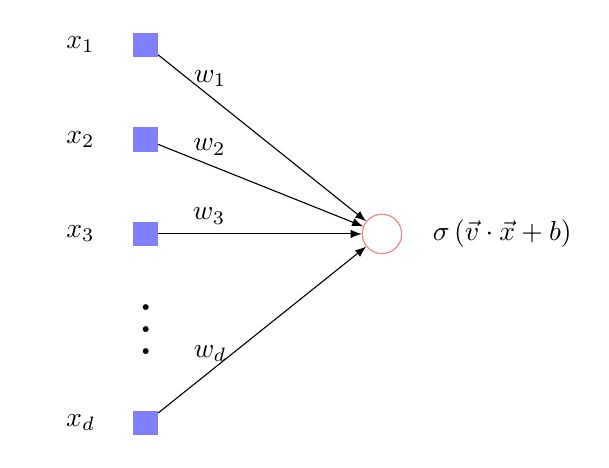
\begin{tikzpicture}[x=1.5cm, y=1.2cm, >=latex]
      \tikzset{
  inputnode/.style={
    rectangle,
    draw,
    minimum size=.3cm
  },
  every neuron/.style={
    circle,
    draw,
    minimum size=.5cm
  },
  neuron missing/.style={
    draw=none, 
    fill=none, %<- added
    scale=2,
    text height=0.333cm,
    execute at begin node=\color{black}$\vdots$
  }
}

\foreach \m [count=\y] in {1,2,3,missing,4} %<- removed "/\l" here 
  \node [fill=black,inputnode/.try, neuron \m/.try,blue!50] (input-\m) at (0,2.5-\y) {};
% added "fill=green" in the line above

\foreach \m [count=\y] in {1}
  \node [every neuron/.try, neuron \m/.try,red!50] (output-\m) at (2,.5-\y) {};

\foreach \l [count=\i] in {1,2,3,d}
  \path (input-\i) -- ++(-1,0)
   node [midway] {$x_\l$};

\foreach \l [count=\i] in {1}
  \path (output-\i) -- ++(1.3,0)
    node [near end] {$\sigma\left(\vec{v}\cdot\vec{x}+b\right)$};

\foreach \i in {1,...,4}
  \foreach \j in {1}
    \draw [->] (input-\i) -- (output-\j);

\foreach \l [count=\i] in {1,2,3,d}
  \foreach \j in {1}
    \path (input-\i) -- (output-\j)
      node [above,near start] {$w_\l$};

% \foreach \l [count=\x from 0] in {Eingangs-, Ausgangs-}
%   \node [align=center, above] at (\x*4,2) {\l \\ Neuronen};
    \end{tikzpicture}
    \caption{perceptron}
    \label{fig:nn_perceptron}
  \end{subfigure}
  \begin{subfigure}{0.495\textwidth}
    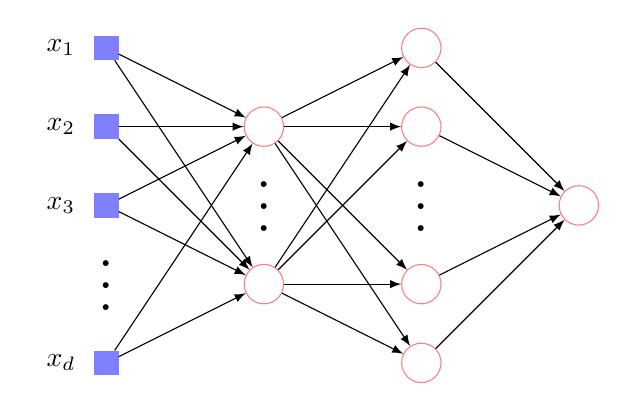
\begin{tikzpicture}[x=1.cm, y=1.cm, >=latex]
      \tikzset{
  inputnode/.style={
    rectangle,
    draw,
    minimum size=.3cm
  },
  every neuron/.style={
    circle,
    draw,
    minimum size=.5cm
  },
  neuron missing/.style={
    draw=none, 
    fill=none, %<- added
    scale=2,
    text height=0.333cm,
    execute at begin node=\color{black}$\vdots$
  }
}

\foreach \m [count=\y] in {1,2,3,missing,4} %<- removed "/\l" here 
  \node [fill=black,inputnode/.try, neuron \m/.try,blue!50] (input-\m) at (0,2.5-\y) {};
% added "fill=green" in the line above

\foreach \m [count=\y] in {1,missing,2}
  \node [every neuron/.try, neuron \m/.try,red!50] (hiddenone-\m) at (2,1.5-\y) {};

\foreach \m [count=\y] in {1,2,missing,3,4}
  \node [every neuron/.try, neuron \m/.try,red!50] (hiddentwo-\m) at (4,2.5-\y) {};

\foreach \m [count=\y] in {1}
  \node [every neuron/.try, neuron \m/.try,red!50] (output-\m) at (6,.5-\y) {};

\foreach \l [count=\i] in {1,2,3,d}
  \path (input-\i) -- ++(-1,0)
   node [midway] {$x_\l$};

% \foreach \l [count=\i] in {1,n}
%   \draw [->] (output-\i) -- ++(1,0)
%    node [above, midway] {$a_\l$};

\foreach \i in {1,...,4}
  \foreach \j in {1,...,2}
   \draw [->] (input-\i) -- (hiddenone-\j);

\foreach \i in {1,...,2}
  \foreach \j in {1,...,4}
    \draw [->] (hiddenone-\i) -- (hiddentwo-\j);

\foreach \i in {1,...,4}
  \foreach \j in {1}
    \draw [->] (hiddentwo-\i) -- (output-\j);

% \foreach \l [count=\x from 0] in {Eingangs-, Ausgangs-}
%   \node [align=center, above] at (\x*4,2) {\l \\ Neuronen};
    \end{tikzpicture}
    \caption{fully connected deep neural network}
    \label{fig:nn_ffnn}
  \end{subfigure}
  \caption{
    schematic view of and perceptron neural networks.
  }
  \label{fig:nn}
\end{figure}
A perceptron can only learn distributions that are linearly separable.

Let's move to the definition of \emph{fast-forward fully connected neural network}.
We can stack neurons in many layers, a neuron takes as input the output of all neurons in the previous layer (the first layer use the input data instead);
the last layer consists of just a neuron whose output is the output of the network.
The topology of the network is defined by the \emph{meta-parameters}: the network will have \(l\) layers with \(f_1,\dots,f_l\) parameters each;
the meta-parameters are fixed before optimization begins and are never changed again.
Writing an explicit formula of the function represented by the neural network is complicated,
it is much more effective to look at the schematic representation in Figure~\ref{fig:nn_ffnn}.
Network parameters are the set of parameters of individual neurons \(\vec{\Theta} = (\vec{\theta}_{1,1},\dots,\vec{\theta}_{l,f_l})\).

Several variants to this construction can be considered (networks not fully connected, different activation functions, parameters shared by multiple neurons, etc.),
but we limit ourselves to this one since for the theoretical approach they are more than sufficient.
\subsubsection{The training algorithm}
Now that we have framed the problem, and the class of predictors we will use to solve it,
we need to define an algorithm that optimizes the neural network parameters to our input data.
Mathematically, we would like to find the network parameters that minimize risk.
One of the most popular algorithms for finding the minimum of a function is gradient descent
\[
  \vec{\Theta}^{\nu+1} = \vec{\Theta}^{\nu} - \gamma \nabla_{\vec{\Theta}} \risk_\text{emp},
\]
where \(\gamma\) is known as learning rate and is one of the \emph{hyper-parameters} of the algorithm.

The algorithm we described is known as \emph{full-batch gradient descent} and is rarely used in practical problems since it has a very large computational cost if \(n\gg1\).
Several solutions have been developed to overcome this issue; the most famous is \emph{stochastic gradient descent},
where the gradient is estimated with a single sample drawn randomly in the training set
\[
  \nabla_{\vec{\Theta}} \risk_\text{emp} \approx \nabla_{\vec{\Theta}}\loss{\left(y_j,\hat{f}{(\vec{x}_j)}\right)}\quad
  \text{where $j$ is random sample in }[1,n].
\]

\subsection{Open question and challenges}
Through the development of the techniques described above, engineers have achieved incredible results with neural networks. However, most of them are due to tricks and hands-on experience, leaving a gap in the theoretical understanding of neural networks.

First, gradient descent converges around a global minimum only if the function to which it is applied is convex.
The empirical risk, however, is deeply nonconvex in the network parameters, with several local minima in the domain.
When this algorithm is applied in practice, though, convergence to a minimum that is at least close to the global minimum is observed.
Some work has gone in the direction of explaining this phenomenon by looking at the landscape of the loss function \cite{sarao2020optimization,sarao2020complex}, but an unambiguous and satisfactory answer has not yet been reached.

Secondly, the generalization ability of neural networks is still not fully understood \cite{zhang2021understanding}.
It is common practice to use architectures with a number of parameters (and thus degrees of freedom) comparable to the size of the training set. This is contrary to some known bounds from statistics, which predict the emergence of overfitting. Yet, this is not the case in neural networks, which are still able to generalize well despite the overabundance of parameters.
The point of this work is precisely to create a model in which a description of the learning process can be derived analytically, with the ultimate goal of demonstrating that \emph{overparametrization} not only does not cause overfitting, but also produces a speed-up of the process.

Being able to solve these and all the other problems that plague neural networks understanding is a hot topic in machine learning research. Not only would it lead to the advancement of theoretical knowledge, but it would be of vital importance for designing ever more efficient algorithms and reaching even more milestones than we currently have.

\section{Statistical physics of learning}
Statistical physics offers tools particularly well suited to theoretically address the study of machine learning models.
As we have seen, in machine learning one must handle probability distributions with very high dimensionality and systems with a considerable number of degrees of freedom,
which exactly the purpose for which statistical physics was developed.

The link between statistical physics and computer science originated well before the advent of machine learning;
techniques such as \emph{simulated~annealling}~\cite{kirkpatrick1983optimization},
have been introduced since the 1970s to solve optimization problems with heuristics inspired by thermodynamics.
The picture of the cooling of a material can give us an intuition of why deep learning is strictly related to statistical physics.
The loss that is optimized for training a neural network is highly non-convex, exactly like the hamiltonian of a glassy system.
When cooling a glass, a different schedule can lead to a very different state of the matter;
in the same way, the algorithm used to descend the loss can take to different solutions for the deep neural network.

Physicists who have worked on machine learning problems have brought a different perspective to that usually used in computer science;
in fact, in the latter it is usual to classify the difficulty of a problem by focusing on the \emph{worst case}.
This viewpoint leads to strong guarantees of success for the model, but at the same time the obtained bounds are very loose and do not reflect what is observed in practical experiments.
In contrast, the results that follow from statistical physics are on the \emph{average case} since we usually tend to consider the thermodynamic limit,
which then becomes a high-dimensional limit.
This description is often closer to experimental observations and that is why it is successful.

Focusing on neural networks, statistical physics has begun work on simplified models of unsupervised learning, and inference more generally, since the 1980s.
Some pioneering work measured \emph{capacities} and \emph{learning~curves} of some simplified nerworks, such as the Hopfield~model~\cite{hopfield1982neural}.
Statistical inference is easylly mapped into statistical physics contest by assuing that the inferedd distribution is a Boltzman distribution.
It can be shown that quantities of interest in the statistical context, such as log-likelihood, represent thermodynamic potentials in the physical context;
all the tools developed by statistical physics can thus be transferred to the study of models si unsupervised learning.
The research field is still very active with several fronts open.
As an example alone, new algorithms for training \emph{restricted boltzmann machines} based on TAP expansion at the second order have recently been introduced,
which perform better than previously known algorithms~\cite{gabrie18training}.

Some work on supervised learning with deep neural networks has been done as well.
The classical replica trick analysis has been applied on simple architectures back in the 80s,
and it is still explored nowdays.
In the 90s the study of the dynamics of a two-layer neural network was first proposed;
in recent years this has been taken up and studied by several authors and will also be the starting point of this paper.

A great work summarizing the history of statistical physics of learning and describing the fronts on which it has been working in recent years was done by Gabrié~\cite{gabrie2020mean}.
We have limited ourselves to a very quick introduction,
hoping to have given an idea of how this field based on statistical physics is one of the most important for the theoretical study of machine learning.


  \chapter{High-dimensional limit of two-layer neural networks} \label{chap:context}
\chaptermark{High-dimensional limit of two-layer NN}

In this Chapter, we introduce the core object of the entire work: \emph{soft committee machines},
a special case of two-layer neural networks.
We also define the dynamics that we are going to study and rephrase the training in terms
of more convenient variables. Using some well-known results in the literature, we derive the 
\emph{ordinary differential equations} describing the process, which will be the starting point 
for all further analysis in the work.

To conclude, we present some results obtained, as an example of 
outcomes using this setting.

\section{The setting}
The setting we are going to present was first introduced by Saad \& Solla \cite{saad1995line}
back in 1995,
and it is often named after them.
In recent years, this framework has been used as starting point in many different papers
\cite{aubin2018committee, goldt2019dynamics,veiga2022phase}.

We are going to do the same in this work; we present the exact same setting of the seminal paper \cite{saad1995line}, while the differences
will appear in the next chapters. We will also briefly expose some more recent results \cite{goldt2019dynamics},
that put some mathematical rigor in the derivation of the differential equations.

\subsection{Online Gradient Descent on Soft Committee Machines}
Let's consider a two-layer neural network, with the input layer of dimension \(d\),
a hidden layer of arbitrary dimension and the output layer constituted by just 1 node.
In addition, the weight between the hidden layer and the output layer are all fixed 
to the same constant; the activation function \(\act(\cdot)\) is applied only in hidden layer nodes.
The assumptions of using one single neuron with fixed weights can be relaxed without any additional effect appearing in the model.
Training the second layer would complicate the notation, without adding value to the analysis we want to conduct;
for reference to work that does not fix the second layer see Goldt et al.\cite{goldt2019dynamics}.
We, therefore, limit our investigation to the simplest model that captures all the effects of interest to us.
\begin{figure}
  \centering
  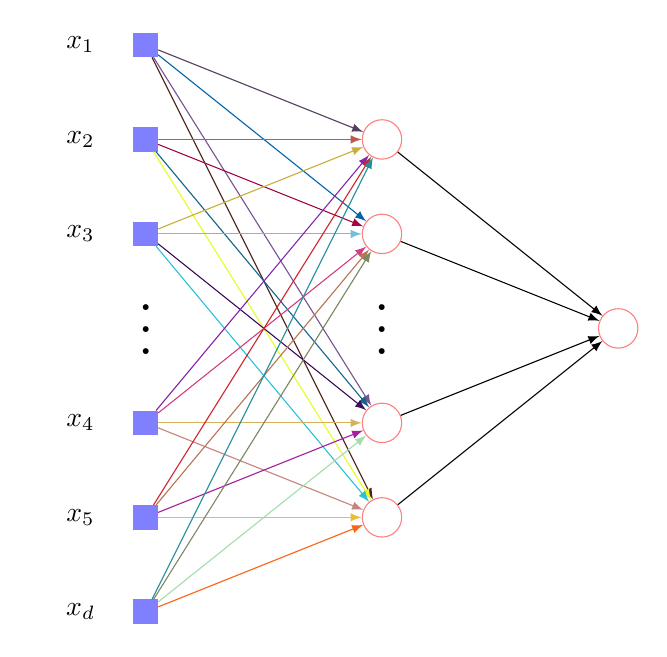
\begin{tikzpicture}[x=1.5cm, y=1.2cm, >=latex]
    \tikzset{
  inputnode/.style={
    rectangle,
    draw,
    minimum size=.3cm
  },
  every neuron/.style={
    circle,
    draw,
    minimum size=.5cm
  },
  neuron missing/.style={
    draw=none, 
    fill=none, %<- added
    scale=2,
    text height=0.333cm,
    execute at begin node=\color{black}$\vdots$
  }
}

\pgfmathparse{rnd}
\xdefinecolor{MyColor}{rgb}{\pgfmathresult, 1.0, 1.0}

\foreach \m [count=\y] in {1,2,3,missing,4,5,6} %<- removed "/\l" here 
  \node [fill=black,inputnode/.try, neuron \m/.try,blue!50] (input-\m) at (0,2.5-\y) {};
% added "fill=green" in the line above

\foreach \m [count=\y] in {1,2,missing,3,4}
  \node [every neuron/.try, neuron \m/.try,red!50] (hidden-\m) at (2,1.5-\y) {};

\foreach \m [count=\y] in {1}
  \node [every neuron/.try, neuron \m/.try,red!50] (output-\m) at (4,-.5-\y) {};

\foreach \l [count=\i] in {1,2,3,4,5,d}
  \path (input-\i) -- ++(-1,0)
   node [midway] {$x_\l$};

% \foreach \l [count=\i] in {1,n}
%   \draw [->] (output-\i) -- ++(1,0)
%    node [above, midway] {$a_\l$};

\foreach \i in {1,...,6}
  \foreach \j in {1,...,4} {
    \edef\R{\pdfuniformdeviate 255}
    \edef\G{\pdfuniformdeviate 255}
    \edef\B{\pdfuniformdeviate 255}
    \xdefinecolor{MyColor}{RGB}{\R,\G,\B}
    \draw [->,MyColor] (input-\i) -- (hidden-\j);
  }


\foreach \i in {1,...,4}
  \foreach \j in {1}
    \draw [->] (hidden-\i) -- (output-\j);

% \foreach \l [count=\x from 0] in {Eingangs-, Ausgangs-}
%   \node [align=center, above] at (\x*4,2) {\l \\ Neuronen};
  \end{tikzpicture}
  \caption{ schematic view of a soft committee machine.
            Different colors represent different weights; the output perceptron has uniform weights.}
\end{figure}
This is known in Statistical Physics literature as the \emph{soft
committee machine}. The name comes from a pictorial representation where every hidden neuron can be seen 
as a member of a committee that independently takes a ``decision'' based on the input;
the final answer of the machine is then obtained by combining the output of the committee
members in a single value. Moreover, the attribute \emph{soft} comes from the fact
that all the members (a.k.a hidden neurons) have the same weight.

We aim to study the training of such a model under some strong assumptions that will
allow us to derive some analytical properties of the entire process.
In particular, we assume the existence of a \emph{teacher} capable to give the output
value at any given input. The teacher is a soft committee machine too, and it is defined 
by a function \(f\colon \Real^d\to\Real\), where \(d\) is the dimension
of the input; the dimension of the teacher's hidden layer is \(k\),
while the matrix of weights \(\W^* \in \Real^{k\times d}\).
The function takes the form
\[
  f{(\vec{x})} = \frac{1}{k}\sum_{r=1}^{k} \act{\left(\frac{\vec{w}^*_r \cdot \vec{x}}{\sqrt{d}}\right)}
  \quad\text{where}\quad \vec{w}^*_r \coloneqq [\W^*]_r \in \Real^d. 
\]
We emphasize that the choice of weights for the second layer was made so that
the output is the average of the values of the hidden neurons. This choice allows
us to compare the output of networks with different hidden layer sizes.
We maintain this convention for all soft committee machines considered in this work.

The machine that are we going to train using the \emph{teacher} output is called \emph{student}.
This particular choice is called \emph{teacher-student setting} and is often used
as a toy model to study the properties of some more complicated problems.
We emphasize that the student knows nothing about the architecture of the teacher.
The teacher is just a convenient generative model for the data and the student observes only the pairs of labels and points,
not the architecture of the teacher.
This might appear as an unfaithful representation of a real situation since it is hardly credible 
that the samples are generated from a model analogous to the one we want to study.
Still, we use this assumption because, as we show later, it allows us to write convenient
variables to monitor and study the learning.
Moreover, in this way we also have the guarantee that the distribution of data is learnable by the student;
if not, we may miss some of the learning steps we want to study.

The student function of course has a similar structure to the teacher.
The only differences are the size of the hidden layer, which is \(p\),
and the weights, which will be  \(\W \in \Real^{d\times p}\). In addition, the weights are not constant
throughout the learning process; we use the apex \(\nu\) to indicate the weights after \(\nu\) steps of learning.
The function of the student is
\[
  \hat{f}^\nu{(\vec{x})} = \frac{1}{p}\sum_{j=1}^{p} \act{\left(\frac{\vec{w}^\nu_j \cdot \vec{x}}{\sqrt{d}}\right)}
  \quad\text{where}\quad \vec{w}^\nu_j \coloneqq [\W^\nu]_j \in \Real^d. 
\]

We make one more assumption in our study: the distribution of the input samples is
normal and independent on each component.
Independence is crucial in order to obtain equations that can be treated analytically,
while the precise distribution is not. 
If desired, we could study non-Gaussian distributions as done by Refinetti~et~al.~\cite{refinetti2022dynamics},
but this would only lead to a complication of calculations, without having a truly more general model.
Moreover, even independence does not make the input used lose generality,
as there are techniques to make the inputs independent, such as principal component analysis.
Using formulas, the samples \(\left(\vec{x}^\nu, y^\nu\right) \in \Real^{d\times1}\) 
used to train the student are chosen as
\[
  \vec{x}^\nu \sim \gauss{(0,\I_d)} \quad\text{ and }\quad 
  y^\nu = f{(\vec{x}^\nu) + \sqrt{\Delta}\xi^\nu}\quad\text{with } \xi^\nu \sim \gauss{(0,1)}.
\]
The value of \(\Delta\ge0\) regulates the noise we are adding to the teacher signal.
The presence of noise is intended to emulate the fact that in a real situation the 
data is not perfect, but it is subject to disturbances of different kinds.
In general, the presence of noise makes the task harder.

The most known and used methods for the neural networks are the many different 
versions of the \emph{gradient descent}. Usually, in supervised learning,
there is a finite dataset where every sample is used in many different learning
steps (possibly all). This reflects the fact that the amount of information accessible
to train the network is finite; it happens more often than you might think, however,
the amount of data available is larger than the amount that can be computed, so one single sample is just used once.
We are going to use what is called the \emph{online gradient descent}
(also known as \emph{one-pass gradient descent}); at each learning step one new sample
is generated from the assumed distribution, used only once and then discarded.
This emulates real situations of data overabundance, but more importantly, it allows us
to write deterministic equations that describe the process since we need the independence
of different learning steps.

Given all the consideration we did and fixing the \emph{learning rate} at \(\gamma>0\),
the update rule of the student weights is
\begin{equation} \label{eq:update_rule_weights}
  \w^{\nu+1}_j = \w^{\nu}_j - \gamma \nabla_{\w_j}\left(\loss\left(y^\nu,\hat{f}^{\nu-1}{\left(\vec{x}^\nu\right)}\right)\right),
\end{equation}
where \(\loss\) is the loss function.
We know that, in order to get the better learning possible, the learning rate should
be chosen so that it decreases as the training progresses, but this does not fundamentally change the stages of learning,
which is ultimately what we want to study; we, therefore, make the choice to hold the learning rate constant for simplicity.
For an analysis that takes into account the possibility of the learning rate varying, see Veiga~et~al.~\cite{veiga2022phase}.

The Equation \eqref{eq:update_rule_weights} is called \emph{update rule for the weights},
and it essentially define a discrete stochastic process. %todo: maybe expand this

The last thing we have to specify for the gradient descent is the loss function \(\loss\).
The choice we did is the \emph{mean squared error}
\[
  \loss{\left(y^\nu,\hat{f}^{\nu-1}{\left(\vec{x}^\nu\right)}\right)} = \frac{1}{2}\left(y^\nu-\hat{f}^{\nu-1}{\left(\vec{x}^\nu\right)}\right)^2.
\]
The final goal of the training is to minimize the \emph{theoretical risk}
(or \emph{population error}), defined as
\begin{equation} \label{eq:theoretical_risk_definition}
  \risk^{\nu} = \E_{\vec{x}\sim\gauss{(0,\I_d)}}{
  \left[\loss{\left(f{\left(\vec{x}\right)},\hat{f}^\nu{\left(\vec{x}\right)}\right)}\right]}=
  \frac{1}{2}\E_{\vec{x}\sim\gauss{(0,\I_d)}}{\left[\left(f{\left(\vec{x}\right)}-\hat{f}^{\nu}{\left(\vec{x}\right)}\right)^2\right]}.
\end{equation}
We have access to this quantity just because we are working in the teacher-student setting.
In real world, one can only monitor the learning using the \emph{empirical risk}, an estimation
of the theoretical one given by the known samples.
This is of course a feature of our artificial setup,
which simply allows us to have complete control of the training.
We emphasize the fact that theoretical risk is not used for the learning step
(it is never the argument of the gradient), but only for monitoring.

We should mention that for the online gradient descent in particular (and not for other types of GD),
the limit \(\gamma\to0\) converges to the gradient flow dynamics on theoretical risk \cite{chizat2019lazy}.
This is a very interesting theoretical fact, which would deserve a separate discussion,
but since we would stray too far from our discussion (we are not studying this limit,
for us the learning rate is a finite quantity), we defer the interested readers to the references.




\subsection{Local Fields and Macroscopic variables}
Looking at the Equation \eqref{eq:theoretical_risk_definition} it's easy to realize
that the risk depends only on the value of the weights, both of the student and of the
teacher. In particular, the weights fully describe the status of a committee machine.
Along the lines of what is done in statistical physics, we would like to define \emph{macroscopic variables}
that do not contain all the information about how the neural network is constructed,
but still be descriptive of its state. In particular, we are interested in expressing
the risk only in function of these variables.
In other words, we are not interested in having control over the state of the weights,
which in thermodynamic language will be the microscopic variables,
but we only need to monitor enough statistics to calculate population risk.

We start the derivation of the macroscopic variables by defining the \emph{local fields}
\[
  \vec{\lf}^{\nu} = \frac{\W^{\nu}\vec{x}}{\sqrt{{d}}} \quad\text{and}\quad
  \vec{\lf}^{*\nu} = \frac{\W^{*}\vec{x}}{\sqrt{{d}}},
\]
where the apices \({\nu+1}\) on \(\vec{x}\) are omitted since they don't matter,
as shown hereafter. These are just the values of the hidden layers, before applying 
the activation function. They are interesting because the whole setting can be rephrased
in terms of the local fields, forgetting the existence of \(\vec{x}^\nu\).
The functions \(f\), \(\hat{f}\) and \(\risk\) depend only on the local fields and not explicitly
on \(\vec{x}^\nu\), therefore it's sufficient to sample and track local fields in order to monitor the learning.
As we already said many times, this is possible just because we are in the artificial
teacher-student setting, but it does not make the analysis less deep.

The \(\vec{\lf}\)s are linear combinations of normal random variables, so they are
normal too. We can then extract some sufficient statics to characterize them.\\
Let's start from the mean, which is particularly straightforward since the \(\vec{x}\)s
are all 0-mean
\[
  \E_{{\vec{x}\sim\gauss{(0,\I_d)}}}{\left[\lf_j^\nu\right]} = \E_{{\vec{x}\sim\gauss{(0,\I_d)}}}{\left[\lf_r^{*\nu}\right]} = 0
  \qquad \forall j\in[p], r\in[k].
\]
It follows that the only quantity needed to characterize the local fields is 
the covariance matrix. 
Let's start with the student-student covariance
\[\begin{split}
  \E_{{\vec{x}\sim\gauss{(0,\I_d)}}}{\left[\lf_j^\nu\lf_l^\nu\right]} &= 
  \E_{{\vec{x}\sim\gauss{(0,\I_d)}}}{\left[\frac1d w_{ja}x_a w_{lb}x_b\right]} =
  \frac1dw_{ja}w_{lb}\E_{{\vec{x}\sim\gauss{(0,\I_d)}}}{\left[x_ax_b\right]}\\ &= 
  \frac1dw_{ja}w_{lb} \delta_{ab} = \frac1dw_{ja}w_{la} = \frac{\left[\W^\nu\W^{\nu\top}\right]_{jl}}{d},\\
\end{split}\]
The other terms are completely analogous
\[
  \E_{{\vec{x}\sim\gauss{(0,\I_d)}}}{\left[\lf_j^\nu\lf_r^{*}\right]} = \frac{\left[\W^\nu\W^{*\top}\right]_{jr}}{d}
  \quad\text{and}\quad
  \E_{{\vec{x}\sim\gauss{(0,\I_d)}}}{\left[\lf_r^*\lf_t^{*}\right]} = \frac{\left[\W^*\W^{*\top}\right]_{rt}}{d}.
\]

The covariance matrices of local fields are a perfect candidate to be
the macroscopic variables we are looking for. Therefore, we give an explicit 
definition of what are known as the \emph{order parameters}
\begin{equation} \label{eq:order_parameters_definiton}
  \Q^\nu \coloneqq \frac{\W^\nu \W^{\nu\top}}{d}, \qquad
  \M^\nu \coloneqq \frac{\W^\nu \W^{*\top}}{d} \quad\text{and}\quad
  \P \coloneqq \frac{\W^* \W^{*\top}}{d}.
\end{equation}
Let us look more closely at these newly defined matrices. \(\Q\) is a square symmetric
matrix of dimension \(p\times p\), where each entry is the overlap between the two
weights of the student. Likewise, \(\P\) is square symmetric, but of dimension \(k\times k\);
it's the auto-overlap of the teacher. Moreover, \(\P\) does not change throughout
the process since the teacher weights are not update. Instead, \(\M\) is a \(p\times k\)
matrix, where each entry is the overlap between a neuron of the teacher and a neuron
of the student. Lastly, \(M\) has more rows than column, the student perfectly 
learns the teacher when has just one non-zero entry per column, each one on a different row.

All covariances can be assembled into a single matrix
\[
  \vec{\Omega}^\nu \coloneqq \left(\begin{array}{cc}
    \Q^\nu & \M^\nu \\
    % \hline
    \M^{\nu\top} & \P
  \end{array}\right).
\]
The matrix \(\vec{\Omega}\in\Real^{(p+k)\times(p+k)}\) is called \emph{overlap matrix} and it fully
describes the learning since it can be used as the covariance matrix for sampling the local fields.
In fact, the local fields at step \(\nu+1\) of the learning can be written as random variables with distribution
\[\vec{\lf}^{\nu+1},\vec{\lf}^{*\nu+1} \sim \gauss{(0,\vec{\Omega}^\nu)}.\]

To conclude this Subsection, we redefine the teacher and the student function
in terms of just the local fields
\[
  f{(\vec{\lf^*})} = \frac{1}{k}\sum_{r=1}^{k} \act{\left(\lf^*_r\right)}\quad\text{and}\quad
  \hat{f}{(\vec{\lf^{\nu}})} = \frac{1}{p}\sum_{j=1}^{p} \act{\left(\lf_j\right)}.
\]
These two lead also to an expression of theoretical risk in terms of overlap matrix only, 
by taking an expected value on local fields
\begin{equation}\label{eq:riskfunctionalOmega}
  \risk{(\vec{\Omega})} = \frac12\E_{\vec{\lf},\vec{\lf^* \sim \gauss{(0,\vec{\Omega})}}}
                              {\left[\left(f{(\vec{\lf}^*)} - f{(\vec{\lf})}\right)^2\right]}
  \quad\text{and}\quad\risk^\nu \equiv \risk{\left(\vec{\Omega}^\nu\right)}.
\end{equation}
We have explicitly expressed the quantity of our interest in terms of the macroscopic 
variables only; the next step is to eliminate the need for weights to describe the learning process.





\subsection{Update rule for overlap matrix} \label{subsec:updateruleforoverlap}
In the previous Subsection, we introduced the order parameters and we showed that 
they are sufficient to describe the status of the learning. We would now like
to write the evolution as a function of only the order parameters,
so we can treat them as the only dynamic quantity of the system.
The goal is therefore to have an update rule for \(\vec{\Omega}\).
First of all, we introduce the \emph{displacement}
\[
  \dsp^\nu \coloneqq f{(\vec{\lf}^*)} - \hat{f}{(\vec{\lf})} + \sqrt{\Delta} \xi^\nu,
\]
as a quantity that just lightens the notation.
Given this definition, the loss function evaluated at \((\vec{x}^\nu,y^\nu)\)
can be simply written as
\[\loss{\left(y^\nu,\hat{f}^{\nu-1}{\left(\vec{x}^\nu\right)}\right)} = \frac{\left(\dsp^\nu\right)^2}{2}.\]
Consequently, the expression of the population risk can be written with this notation As
\begin{equation}\label{eq:risk_lambda_expval}
  \risk{(\vec{\Omega})} = \frac12\E_{\vec{\lf},\vec{\lf^* \sim \gauss{(0,\vec{\Omega})}}}
                              {\left[\left(\dsp^\nu\right)^2\right]}.
\end{equation}

The second step is to explicitly compute the gradient of the loss respect to the weights
\[
  \nabla_{\w_j}\left(\frac{\left(\dsp^\nu\right)^2}{2}\right) =
    -\dsp^\nu \nabla_{\w_j}\left(\hat{f}{\left(\vec{\lf_j}\right)}\right) =
    -\dsp^\nu \frac{\act'{\left(\vec{\lf}^\nu_j\right)}}{p}\frac{\vec{x}^\nu}{\sqrt{d}} =
    -\frac{1}{p}\dsp^\nu_j \frac{\vec{x}^\nu}{\sqrt{d}},
\]
where in the last step we used another notation shorthand
\[
  \dsp^\nu_j \coloneqq \act'{(\lambda_j^\nu)} \dsp^\nu.
\]
We stress out the fact that all the \(\dsp\) and \(\dsp^\nu\) are in the end function of only
the local fields.

Indeed, it follows from Equation \eqref{eq:update_rule_weights} that the update rule
for the weights still depends on the sample \(\vec{x}^\nu\)
\[
  \w^{\nu+1}_j = \w^{\nu}_j + \frac{\gamma}{p} \dsp^\nu_j \frac{\vec{x}^\nu}{\sqrt{d}}.
\]

We can now use this to derive the update rules for the order parameters.
Let's start from \(\M\)
\begin{equation} \label{eq:update_rule_M}
  \left[\M^{\nu+1}\right]_{jr} = \frac{\w^{\nu+1}_j \w^{*\top}_r}{d}
    = \frac{\w^{\nu}_j \w^{*\top}_r}{d} + \frac{\gamma}{dp} \dsp^\nu_j \frac{\vec{x}^\nu}{\sqrt{d}}\w^{*\top}_r
    = \left[\M^{\nu}\right]_{jr} + \frac{\gamma}{dp} \dsp^\nu_j \lf_r^*,
\end{equation}
that is not explicitly dependent in \(\vec{x}\) or \(\vec{w}\). The computation
for the \(\Q\) update rule is a little bit more complex
\begin{equation}\label{eq:update_rule_Q}\begin{split}
  \left[\Q^{\nu+1}\right]_{jl} &= \frac{\w^{\nu+1}_j \w^{\nu+1\top}_l}{d}
    = \frac{\w^{\nu}_j \w^{\nu\top}_l}{d} + \frac{\gamma}{pd} \dsp^\nu_j \frac{\vec{x}^\nu}{\sqrt{d}}\w_l^\nu
      + \frac{\gamma}{pd} \dsp^\nu_l \frac{\vec{x}^\nu}{\sqrt{d}}\w_j^\nu 
      + \frac{\gamma^2}{p^2d} \dsp^\nu_j\dsp^\nu_l \frac{\left(\vec{x}^\nu\right)^2}{d}\\
    &= \left[\Q^{\nu}\right]_{jl} + \frac{\gamma}{pd}\left(\dsp^\nu_j \lf_l^\nu + \dsp^\nu_l \lf_j^\nu\right)
    + \frac{\gamma^2}{p^2d} \dsp^\nu_j\dsp^\nu_l \frac{\left(\vec{x}^\nu\right)^2}{d}.
\end{split}\end{equation}
We notice that the update rule still depends explicitly on \(\vec{x}^\nu\).
Apparently, this dependence prevents us from being able to write an update rule
that depends only on order parameters and local fields, but, as we show now, the 
high-dimensional is of help.
In fact, the factor \(\frac{\left(\vec{x}^\nu\right)^2}{d}\) goes to 1 and 
fluctuations can be neglected, in the limit of large \(d\) and fixed \(p,k,\gamma\) and \(\Delta\)\footnote{
  \(\left(\vec{x}^\nu\right)^2\) is distributed as a Chi-square with \(d\) degrees
  of freedom, so for large \(d\) we have 
  \(\frac{\left(\vec{x}^\nu\right)^2}{d} \sim \gauss{\left(1,\frac1d\right)}\).

  Although it is a passage often found in the literature,
  this statement is not obvious and especially not rigorous.
  For simplicity's sake, we report as it is.
  In the next section we will give a formal justification on how to go from update rule
  to differential equations; the theorem we present also includes this unclear step.
}. Consequently, as of now, we will no longer write this term, assuming it has been replaced by 1.

In conclusion, learning can be described as a \emph{discrete stochastic process}
on the overlap matrix
\[\left\{\vec{\Omega}^\nu \in \Real^{(p+k)\times(p+k)}|\nu\in\Natural\right\},\]
and the risk is just a function of \(\vec{\Omega}\), as shown in Equation~\eqref{eq:riskfunctionalOmega}.
We succeeded in transforming our setting built to study the learning of a neural network,
in a simpler stochastic process of some macroscopic variables, that do not fully characterize
the network, but still give enough information for further analysis.





\subsection{High-dimensional limit}
In this Subsection we proceed in expressing the most important result of Saad\&Solla\cite{saad1995line}:
the derivation of \emph{ordinary differential equations} whose solution can be used
to approximate the stochastic process of the order parameters. 

We first present a derivation \emph{à la physicist}, that gives a great intuition of what is going on,
but it lacks mathematical rigor. After that, we briefly present some recent results that
formalize the idea.
We stick to the Saad-Solla regime, where there is no dependence in \(d\) of \(p\) and \(\gamma\).

The thing to point out is how to pass from a discrete process to a time-continuous equation.
In other words, we need a mapping from the step number \(\nu\) to a time \(t\) such that
the discretization becomes finer and finer the closer we approach the limit of higher dimension.
The update rules for the macroscopic variables can be manipulated to obtain
\begin{subequations}\label{eq:order_param_discrete_derivative}\begin{align}
  \frac{\left[\M^{\nu+1}\right]_{jr} - \left[\M^{\nu}\right]_{jr}}{\frac1d} &= \frac{\gamma}{p} \dsp^\nu_j \lf_r^*\\
  \frac{\left[\Q^{\nu+1}\right]_{jl} - \left[\Q^{\nu}\right]_{jl}}{\frac1d} &=
    \frac{\gamma}{p}\left(\dsp^\nu_j \lf_l^\nu + \dsp^\nu_l \lf_j^\nu\right) + \frac{\gamma^2}{p^2} \dsp^\nu_j\dsp^\nu_l.
\end{align}\end{subequations}
If we force the left-hand side to become a derivative in the limit, the natural choice at this point is the time scaling is
\[t=\frac{\nu}{d} \quad\text{and}\quad \delta{t} =\frac1d.\]
We now have to take the limit for \(d\to\infty\) (or analogously \(\delta t \to 0\))
As already said, the LHSs of the equations above turn into a continuous time derivative.
The tricky part is the right-hand side: the increase of dimension can be seen as 
an increase of i.i.d. random variables on which average on. This picture is true
because the \(\vec{x}\) only appears through local fields, where is first scalar-multiplied
by a weights vector, and then divided by a scaling \(\sqrt{d}\). 
% \todo{Questa parte é spiegata con i piedi!}
We can then invoke a heuristic version of the central limit theorem,
and state that the random variables appearing at the RHS converge in the limit
to their expected value. All these claims turn out to be true, so we can finally write
\begin{subequations}\label{eq:genericODE}\begin{align}
  \label{eq:genericODEforM}
  \dod{\left[\M{\left(t\right)}\right]_{jr}}{t} &=\E_{\vec{\lf},\vec{\lf^* \sim \gauss{(0,\vec{\Omega}{(t)})}}}{\left[\frac{\gamma}{p} \dsp_j \lf_r^*\right]} \eqqcolon \Psi_{jr}{\left(\vec{\Omega}\right)}\\
  \label{eq:genericODEforQ}
  \dod{\left[\Q{\left(t\right)}\right]_{jl}}{t} &=\E_{\vec{\lf},\vec{\lf^* \sim \gauss{(0,\vec{\Omega}{(t)})}}}{\left[\frac{\gamma}{p}\left(\dsp_j \lf_l + \dsp_l \lf_j\right) + \frac{\gamma^2}{p^2} \dsp_j\dsp_l\right]} \eqqcolon \Phi_{jl}{\left(\vec{\Omega}\right)},
\end{align}\end{subequations}
where we have also defined the two matrix function \(\vec{\Psi}\colon\Real^{(p+k)\times(p+k)} \to\Real^{p\times k}\) and 
\(\vec{\Phi}\colon\Real^{(p+k)\times(p+k)} \to\Real^{p\times p}\).
They are well-defined because the local fields are 0-mean gaussian, so any statics
can only depend on their covariance matrices.

In short, the discrete stochastic process has turned into a continuous deterministic evolution.
For some choices of the activation function, the expectations can be computed analytically and
the so derived system of ordinary differential equations can be studied in order
to understand the learning process.

\subsubsection{Formal derivation}
In this part, we briefly present an important result by Goldt et al.\cite{goldt2019dynamics}
that achieves to give some mathematical rigor to the derivation of the differential
equations. It also provides a bound on the maximum expected error between the process
and the equations' solution. We are not going to report the full proof, but just 
present the main theorem, explaining clearly all the hypotheses and regimes in which
it is applicable.

The original Theorem is valid for any kind of committee machine, but we only present
an adaptation to the \emph{soft} case, to be consistent with the notation
we introduced in the previous sections.
\begin{Theorem}\label{thm:process_to_ode_goldt}
  Let's suppose that
  \begin{enumerate}
    \item The function \(\sigma\) is bounded and its derivatives up to the second order exist and are bounded, too;
    \item The initial macroscopic state \(\vec{\Omega^0}\) is deterministic and bounded by a constant;
    \item The constants \(\Delta, p, k\) and \(\gamma\) are all finite.
  \end{enumerate}
  Let \(T>0\), then the overlap matrix satisfies 
  \begin{equation}
    \max_{0\le\nu\le Td} \E\left[
      \left\|\vec{\Omega}^\nu - \tilde{\vec{\Omega}}\left(\frac{\nu}{d}\right)\right\|
    \right]
    \le
    \frac{C{(T)}}{\sqrt{d}},
  \end{equation}
  where \(\tilde{\vec{\Omega}}\) it's the unique solution of the Equations \eqref{eq:genericODE},
  with the initial condition \(\tilde{\vec{\Omega}}{(0)} = \vec{\Omega}^0\). 
\end{Theorem}
The important part is that the constant \(C{(T)}\) does not depend on \(T\), thus 
the theorem proves the convergence of the ODEs solution to the stochastic process.
The proof can be found in the original paper\cite{goldt2019dynamics};
it is strongly based on some techniques introduced by Wang in some previous works
\cite{wang2017scaling,wang2019solvable}.

Thanks to the Theorem, we have formal proof that the well-known Equations~\eqref{eq:genericODE}
can be used to analyze the learning of a committee machine. From this point,
we assume the \emph{differential equations} to be descriptive of our system,
and we will use them to derive different kinds of results.

%todo: forse bisognerebbe dire altro, ma per ora mi va bene cosí.



\section{Example: Phase Diagram of Soft Committee Machine}
In this Section, we are going to present the results obtained by Veiga et al.\cite{veiga2022phase},
as an example of the application of all the tools introduced in the previous section.
This paper was the starting point for the work we present in this thesis;
discussions with the authors helped to arrive at the results of this thesis.
Therefore, we believe that reporting the results can likewise help the understanding of the next chapters,
as well as show the potential of the tools we have just exposed.

The setting we presented in the last Section assumed that \(p\) and \(\gamma\) were constant when the limit \(d\to\infty\) was calculated.
The purpose of the paper is to extend this analysis to the case where both network width and learning rate depend polynomially on \(d\).
We arrive at drawing a phase diagram for the final state of learning as a function of the scaling exponents of \(p\) and \(d\).

Suppose that \(p\) and \(\gamma\) vary as a function of \(d\) as
\[p=p_0 d^\kappa\quad\text{and}\quad\gamma=\gamma_0d^{-\delta}.\]
All the derivation made in the previous section, up to before the limit procedure,
also applies when using the substitutions above. We can then rewrite the Equations~\eqref{eq:order_param_discrete_derivative}
in this context
\begin{subequations}\label{eq:order_param_discrete_derivative}\begin{align}
  \left[\M^{\nu+1}\right]_{jr} - \left[\M^{\nu}\right]_{jr} &= \frac{1}{d^{1+\kappa+\delta}}\frac{\gamma_0}{p_0} \dsp^\nu_j \lf_r^*,\\
  \left[\Q^{\nu+1}\right]_{jl} - \left[\Q^{\nu}\right]_{jl} &=
  \frac{1}{d^{1+\kappa+\delta}}\frac{\gamma_0}{p_0}\left(\dsp^\nu_j \lf_l^\nu + \dsp^\nu_l \lf_j^\nu\right) + \frac{1}{d^{1+2(\kappa+\delta)}}\frac{\gamma_0^2}{p_0^2} \dsp^\nu_j\dsp^\nu_l.
\end{align}\end{subequations}
The time differential that is used to make the limit is no longer simply \(1/d\),
but depends explicitly on \(\kappa\) and \(\delta\)
\[
  \delta t = \max\left(\frac{1}{d^{1+\kappa+\delta}}, \frac{1}{d^{1+2(\kappa+\delta)}}\right).
\]
What happens when we go to the limit \(d\to+\infty\) is that, depending on the value of \(\kappa+\delta\),
some terms in the equations are suppressed, thus leading to very different differential equations and consequently different results in learning.
We can distinguish the following 4 regimes:
\begin{itemize}
  \item \emph{Plateau} \(\kappa = -\delta\): the equations obtained are exactly the same as the previous Section.
        The learning process converges to a plateau related to the noise value.
        In any case, the result has been extended, since we previously knew it was valid only for \(\kappa=\delta=0\);
  \item \emph{Perfect Learning} \(\kappa > -\delta\): the risk at the end of the learning process goes to zero, even in the presence of noise.
  \item \emph{Bad learning} \(-\frac12<\kappa+\delta<0\): the linear terms in \(\gamma_0/p_0\) in the equations are suppressed;
        the noise dominates the learning process and it's not guaranteed that the final value of the risk is smaller than the starting value.
  \item \emph{No ODEs} \(\kappa+\delta<-\frac12\): the stochastic process can't be described with ODEs, since some terms does not concentrate.
\end{itemize}
\begin{figure}
  \centering
  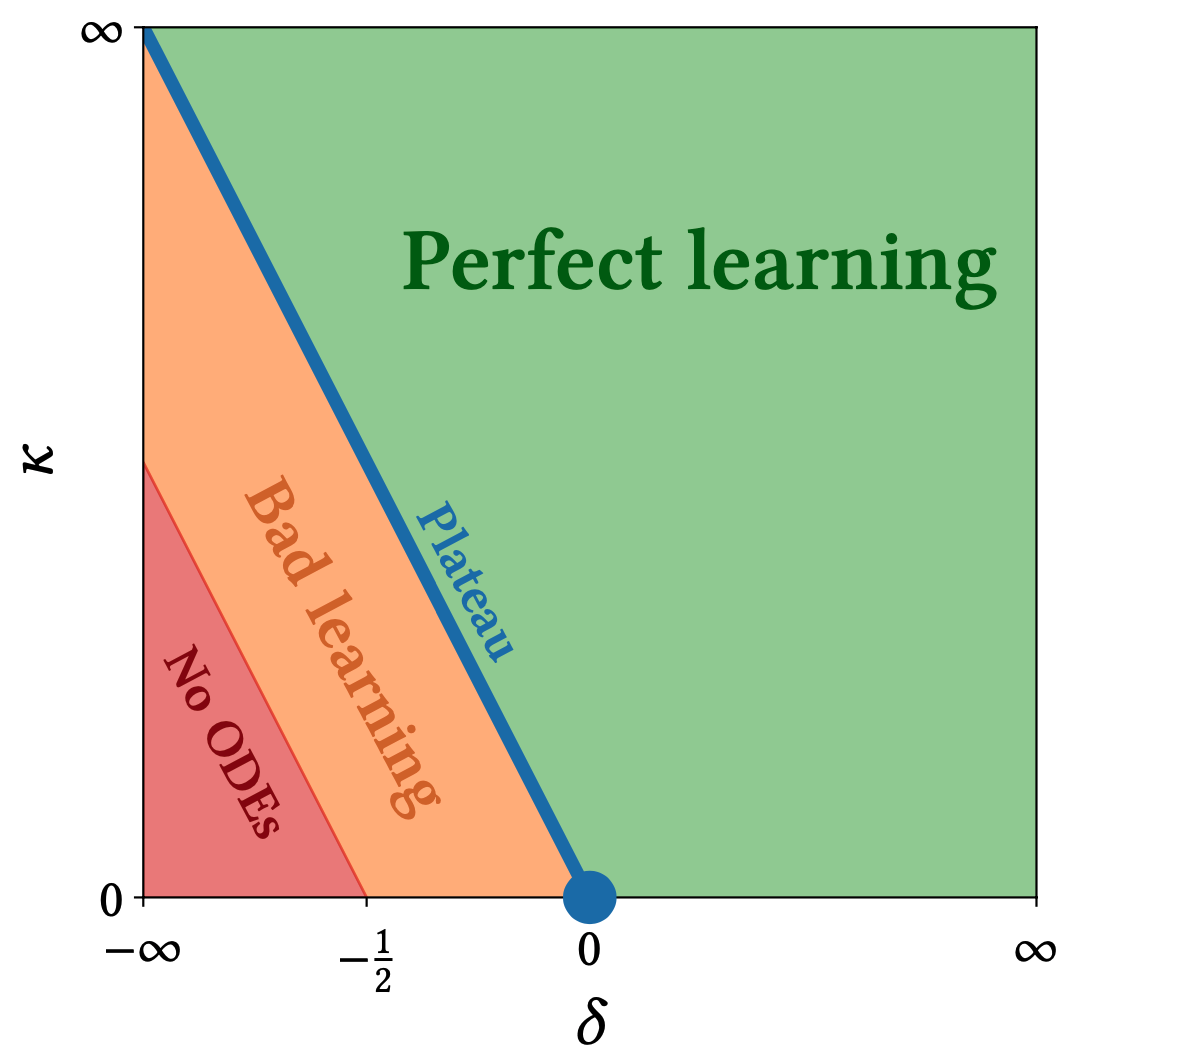
\includegraphics[width=0.7\textwidth]{figures/veiga_phase_diagram.png}
  \caption{
    schematic phase diagram showing the different regimes.
    Source~\cite{veiga2022phase}.
  }
  \label{fig:veiga_phase_diagram}
\end{figure}
\begin{figure}
  \centering
  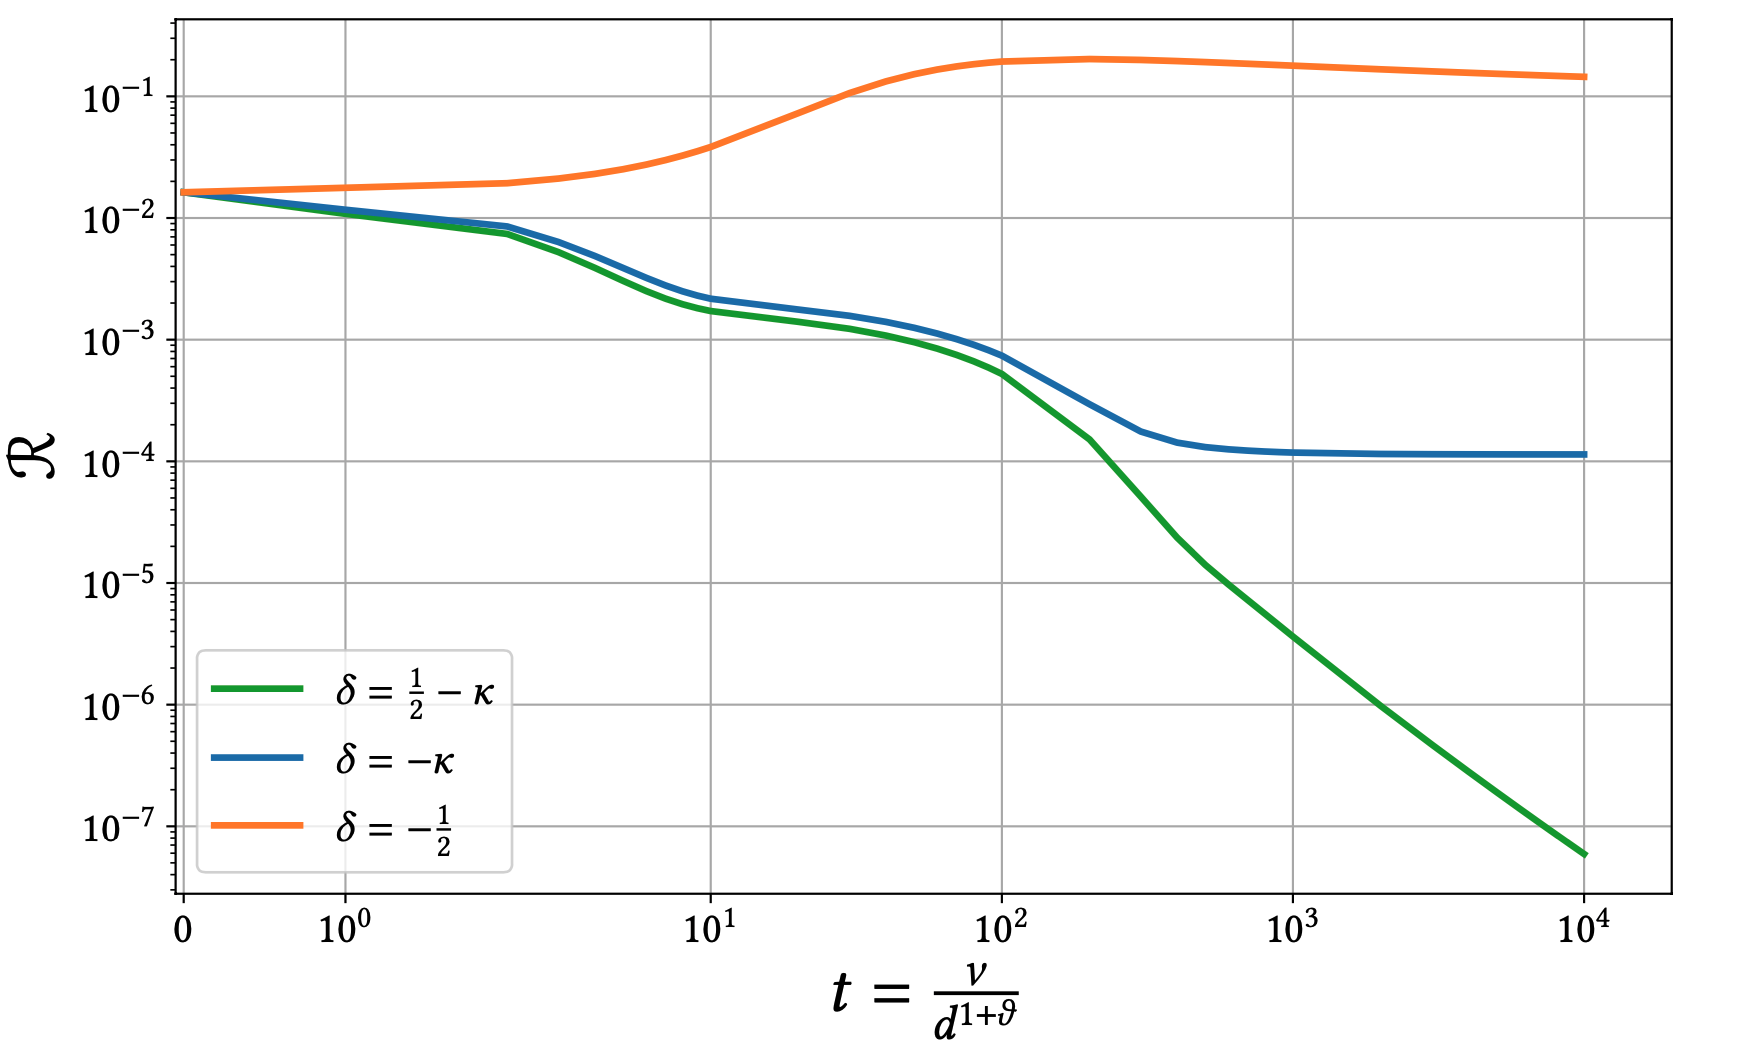
\includegraphics[width=0.9\textwidth]{figures/veiga_traj_examples.png}
  \caption{
    example of trajectories in different regimes. Yellow: bad learning; blue: plateau; green: perfect learning.
    Source~\cite{veiga2022phase}.
  }
  \label{fig:veiga_traj_examples}
\end{figure}
Figure~\ref{fig:veiga_phase_diagram} is a schematic representation that summarizes the 4 different regimes.
Figure~\ref{fig:veiga_traj_examples} shows simulated trajectories in different regimes, supporting what we presented.
The interesting thing is that if the learning rate decreases you always have perfect learning; however, this is not a necessary condition: if the network is large enough even if the learning rate diverges you can still have perfect learning.

We also note that the case we are going to study (\(\kappa=\delta=0\)) is in a very special regime ``on the edge of learning''.
We, however, will not be interested in the end state, but we would like to study the dynamics leading up to it.
In particular, we will focus on estimating the transition times of the various stages of learning.


  \part{Results}
  \chapter{Quadratic activation and initial conditions}
In this chapter, we introduce the first part of the original work of this thesis.
We further develop the framework introduced in previous chapters;
we will set an unusual activation function, but one that will allow us to derive
tractable equations for our purposes.

After that, we exhibit the code used for the simulation of the learning, and the differential
equation solution. 

Finally, we discuss the problem of the initial condition. Choosing the proper starting
point is one of the most challenging parts of this work. We briefly report our first
attempts to address the problem, leaving instead for the next chapter
the final choice.

\section{Quadratic activation function}
In the last chapter, we introduced the generic framework for studying soft committee machines.
We derived some generic differential equations, which, however, involve calculating an expectation value.
If the purpose is an analytical study of the process, it is necessary to find an explicit expression
for those values of expectation, otherwise, the study is arduous.

In previous literature\cite{saad1995line,goldt2019dynamics,veiga2022phase}, the standard choice in this case is
\[\sigma{(x)} = \erf{\left(\frac{x}{\sqrt{2}}\right)},\]
where \(\erf\) is the \emph{error function}. This choice is particularly convenient
because \(\erf\) is a regular and bound function, and its derivative is the gaussian.
The resulting expected values are computable; this is not clearly true for other 
common choices such as \emph{sigmoid} or \(\tanh\).

%todo: As an example, we report here what is Equation~\eqref{eq:genericODEforM} for this activation function.
Nevertheless, the expression obtained by computing the expected values in Equations~\eqref{eq:genericODE} involves
some inverse trigonometric functions, square roots and some other non-simple expressions. For reference, see
the Appendix~C of Veiga's paper\cite{veiga2022phase}, where the full expressions are reported.
Our ultimate goal is to derive analytical estimates of the learning times of the committee machines;
to do this we need the differential equations to be relatively simple and tractable with analytical techniques,
which unfortunately is not true with the canonical choice of \(\sigma\).
\begin{figure}
  \centering
  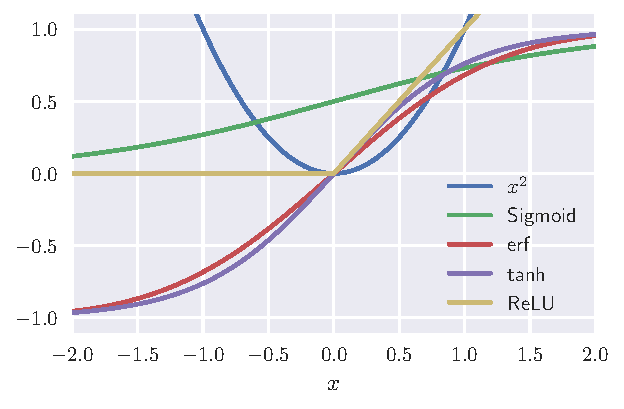
\includegraphics[width=0.7\textwidth]{figures/activation_function.pdf}
  \caption{ different choice of activation function.}
\end{figure}

Thus, the problem is now choosing a new activation function that would allow for more tractable equations.
The most natural choice is one with polynomial \(\sigma\). The simplest polynomial would be \(\sigma(x) = x\),
but it's well known that using a linear activation function in hidden layers leads to just a linear function,
so there is no point to use neural networks at all\cite{szandala2021review}\footnote{
  Actually, even if a deep neural network with linear activation is equivalent to a linear function, this does not mean that the dynamics of learning is the same as the corresponding function. See \cite{saxe2013exact} for reference. However, it is not of our interest to study the dynamics of a linear network.
}. 
Given all these considerations, the choice we did is \[\act{(x)} = x^2.\]
We need to point out a few things at this point.
First of all, the quadratic function, as well as all the other polynomial functions,
does not satisfies the Hypothesis~1 of Theorem~\ref{thm:process_to_ode_goldt}.
This seems to break the convergence of the differential equations solution to the
stochastic process of the training.
However, the fact that our condition violates the theorem does not necessarily imply that it is not true in this case. Following a discussion with the authors of the theorem, we have sufficient reason to believe that the proof can be extended to our activation function as well;
lipschitzianity was taken as a convenient assumption for the proof, but it is not the strictest condition we can have. We can also imagine truncating the parabola above a certain threshold, making the activation technically lipschitz.

Secondly, the usage of an even function as activation introduces an unusual symmetry in 
the functions. Both the student \(\hat{f}\) and the teacher \(f\) are even functions,
thus the sign of all the weights of a single neuron can be changed, without changing 
the output. In the macroscopic variables framework, this results in a loss of significance
of the sign of nondiagonal elements of \(\Q\) and \(\P\), and of all entries of \(\M\).
It follows that all these signs in the final state are determined by the choice of initial
conditions, and a small variation of those can lead to opposite solutions. This effect 
will mildly affect our analysis; we will point out this again when needed.

Finally, we notice that all the expected values we need to compute are just multivariate
polynomials of gaussian variables. The final result is particularly nice
because it is a polynomial in the covariance matrix entrances. The full derivation
is reported in Appendix~\ref{app:derivation-quadratic-ode}.
We report below the final expression of the equations.
\begin{subequations} \label{eq:quadraticODEs}\begin{align}
    \label{eq:quadraticODE_M}
    \dod{\M}{t} &= \frac{2 \gamma}{p}\left[
        \left(\frac{\Tr{\P}}k - \frac{\Tr{\Q}}p\right)\M +
        2\left(\frac{\M\P}{k} - \frac{\Q\M}{p}\right)
    \right] \\
    %
    \label{eq:quadraticODE_Q}
    \begin{split}
        \dod{\Q}{t} &= \frac{4 \gamma}{p}\left[
            \left(\frac{\Tr{\P}}k - \frac{\Tr{\Q}}p\right)\Q +
            2\left(\frac{\M\M^\top}{k} - \frac{\Q^2}{p}\right)
        \right] +\\
        &\quad+\frac{4 \gamma^2}{p^2} \Biggr\{
            \frac1{k^2}\left[\left(\Tr{\P}^2+2\Tr{\P^2}\right)\Q +
                            4\Tr{\P}\M\M^\top + 8\M\P\M^\top
                    \right] - \\
            &\qquad\quad\quad
            -\frac2{kp}\Biggl[\left(\Tr{\P}\Tr{\Q}+2\Tr{\M\M^\top}\right)\Q +
                            2\Tr{\Q}\M\M^\top\\
                            &\qquad\qquad\qquad\quad+ 2\Tr{\P}\Q^2+ 
                            4\left(\M\M^\top\Q + \Q\M\M^\top\right)
                        \Biggl] + \\
            &\qquad\quad\quad
            +\frac1{p^2}\left[\left(\Tr{\Q}^2+2\Tr{\Q^2}\right)\Q +
                            4\Tr{\Q}\Q^2 + 8\Q^3
                        \right] + \Delta \Q\Biggr\}
    \end{split}
\end{align}\end{subequations}
The expressions are just long, but not complicated to handle and to be analyzed.
% Moreover, these are their compact matrix form

To conclude our specialization in quadratic activation, also the value of population risk can be expressed
as function of the values of \(\Q, \M \text{ and } \P\). Computing the expected value in Equation~\eqref{eq:risk_lambda_expval},
we get
\begin{equation} \label{eq:risk_quadratic}\begin{split}
  \risk%{(\Q,\M,\P)}
      = \frac12\Bigg[&
          \frac{\Tr{\P}^2+2\Tr{\P^2}}{k^2}
          -2\frac{\Tr{\P}\Tr{\Q}+2\Tr{\M\M^\top}}{pk} \\
          &+\frac{\Tr{\Q}^2+2\Tr{\Q^2}}{p^2}
      \Bigg]
\end{split}\end{equation}

The equation derived will be the starting point for all further analysis.
We are using an unusual choice of activation function, but, as presented later,
we will be still able to recover known results in the literature, and derive some original
ones.

\subsection{Special case: Phase Retrieval}\label{subsec:phase_retrieval}
In this subsection, we briefly present the \emph{phase retrieval} model,
since it is a special case of our framework and consequently we will use it often in further work.

Suppose we want to learn a model defined by 
a single vector \(\vec{w}^* \in \Real^d\) and the function represented by this model is 
\[
  f\colon \Real^d \to \Real^+ \qquad f{(\vec{x})} = \left(\frac{\vec{w}^*\cdot\vec{x}}{\sqrt{d}}\right)^2.
\]
In our setting, phase retrieval corresponds to the case \(k=1\). The task is notoriously
harder than the counterpart without the square, since there is no access to the sign of 
the scalar product\footnote{
  The name \emph{phase retrieval} comes from the complex version of this problem (\(f\colon \Complex^d \to \Real^+\)),
  since the hard part of the task is to determine the phases of the vector \(\vec{w}\in\Complex^d\).
}. This corresponds to practical settings, for example in reconstruction problems coming from physics or chemistry, where one often only measures amplitudes and wants to recover the phases or signs.

The classic definition of phase retrieval can be thought of as a teacher-student setting, where we want to learn
a single vector \(\vec{w}\). Similar to before, the student function 
\[
  \hat{f}\colon \Real^d \to \Real^+ \qquad \hat{f}{(\vec{x})} = \left(\frac{\vec{w}\cdot\vec{x}}{\sqrt{d}}\right)^2.
\]
corresponds to the fixing \(p=1\) in our setting. 

Many different algorithms can be used to solve this task, such as 
\emph{full-batch SGD} \cite{mignacco2021stochasticity},
\emph{spectral methods} \cite{mondelli2018fundamental} and 
\emph{approximate message passing} \cite{maillard2020phase}.
As done in the rest of this work, we will focus on the online stochastic gradient descent;
it has been done in the past using both full-batch gradient descent \cite{sarao2020complex,sarao2020optimization},
or online gradient descent~\cite{tan2019online}, but we explore different regimes.
We focus on the study of timings in the high dimensional limit dynamics,
using the square loss.

\subsubsection{Differential equations}
For completeness, we can specialize the Equations~\eqref{eq:quadraticODEs} to the phase retrieval.
This will be helpful in further analyses.

Let's start by observing that all \(\Q\), \(\M\) and \(\P\) are \(1\times 1\) matrices,
so we can substitute them with scalar values
\[\rho \coloneqq \P, \qquad m{(t)}\coloneqq\M{(t)}\quad\text{and}\quad q{(t)}\coloneqq\Q{(t)}.\]
We are now ready to substitute these definitions, together with \(p,k = 1\), into the differential
equations above to get
\begin{subequations}\label{eq:phase_retrieval}\begin{align}
  \dod{m{(t)}}{t} &= 6 \gamma m{(t)} \left(\rho-q{(t)}\right), \\
  \begin{split}
    \dod{q{(t)}}{t} &= 4 \gamma\left(
        \rho q{(t)} + 2m^2{(t)} - 3q^2{(t)}
    \right) +\\
    &\quad+4 \gamma^2 \left[
      3\rho^2q{(t)} + 12\rho m^2{(t)} -6\rho q^2{(t)} -24m^2{(t)}q{(t)} + 15q^3{(t)} + \Delta q{(t)}\right].
  \end{split}
\end{align}\end{subequations}
This system of two coupled differential equations fully describes the learning in the case of phase retrieval.

To conclude, here is also the risk expression for the phase retrieval
\begin{equation}
  \risk{(q,m,\rho)} = \frac12\left[3\rho^2-2\rho q - 4m^2 + 3q^2\right].
\end{equation}

\section{Numerical Experiments setting}
In this section, we describe how we conducted the numerical experiments to verify 
our results. We discuss some common problems that need to be addressed in every kind of simulation,
while the issues specific to an individual task will be discussed in the appropriate section.

All the code written for this work is contained in this \Href{https://github.com/arn4/master-thesis/tree/main/code/committee_learning_package}{Python package}.
It can be downloaded and the experiments can be reproduced.


\subsection{Simulation of the training}
As we already said, the training of a committee machine looked at through the order parameters
reduces to a discrete stochastic process of the matrix \(\vec{\Omega}\). Thus, one possibility
to simulate the online learning is using Equations~\eqref{eq:update_rule_M} and \eqref{eq:update_rule_Q}:
at each step, the local fields can be sampled using the previous overlapping matrix, then
used to compute the update step. Although this is perfectly allowed, we preferred
to simulate the process directly on the weights, using Equation~\eqref{eq:update_rule_weights}
and sampling each time a new \(\vec{x}\).

Besides being much closer to what is done in practice, using weights gives us much more control over
the committee machine, especially over the initial conditions. 
As we will see better in the next section, the choice of initial conditions is far from trivial,
and imposing them directly on macroscopic variables could lead to unrealistic situations in practice.

Since we wanted to be as close as possible to how a neural network is trained,
we decided to use an external package to handle gradient descent: \texttt{PyTorch}\cite{pytorch2019}.
This ensures that no bias is introduced by our work, since everything in the simulation,
from step update to gradient computation, is handled by the external library.
Moreover, the code is much more general and can easily be adapted to different activation
functions, for instance\footnote{
    In the first stage of the project, we conducted some tests using \(\erf\) activation and compared
    our result to \cite{veiga2022phase}, to be sure that the code is correct.
}.

\subsubsection{Measure of the Population risk}
The quantity we are interested in is the \emph{population risk}, so we have to find
a way to monitor it through the learning. In real neural network training, there is 
no access to the population risk, but only the empirical version can be computed.
We can imagine doing the same in our framework, sampling a set \(\{\vec{x}_1,\dots,\vec{x_N}\}\) 
and using it to estimate the risk
\[\risk = \frac{1}{2N}\sum_{n=1}^N\left(\hat{f}(\vec{x}_n)-f(\vec{x}_n)\right)^2.\]
Of course, the thing to do is sample a new set of \(\vec{x}\)s each time we need an estimation
of the risk, but this strategy turned out to be computationally too expensive to be
implemented with a sufficient amount of samples to have a good estimation.

A second possible strategy is to use the same set \(\{\vec{x}_1,\dots,\vec{x_N}\}\) 
throughout the learning. This solution is introducing a bias because the resulting risk
will always have the same type of error since the samples used are identical.

Although the choice is good for some experiments, it turned out to be not accurate enough
for all the analysis we needed. Therefore we introduced a third way to compute the population 
risk, by first calculating the order parameters, and then applying the Equation~\eqref{eq:risk_quadratic}.
In this way we get an exact expression of the risk;
we are aware that this comes out of the pattern of wanting to emulate a real training of a neural network as much as possible,
but nevertheless, this choice does not impact the gradient descent in any way since
the risk is used just for monitoring.
Finally, let us remember that our goal is to provide an analytical estimate of the committee machine's learning time,
so it is much more important to have accurate numerical results with which to make comparisons,
rather than to be consistent with a real situation.
\begin{figure}
  \centering
  \begin{subfigure}{0.495\textwidth}
    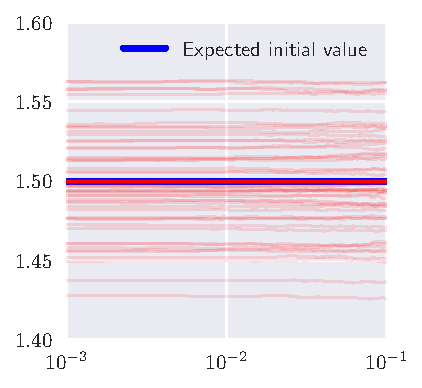
\includegraphics[width=1.\textwidth]{figures/risk_samples.pdf}
    \caption{samples estimation}
  \end{subfigure}
  \begin{subfigure}{0.495\textwidth}
    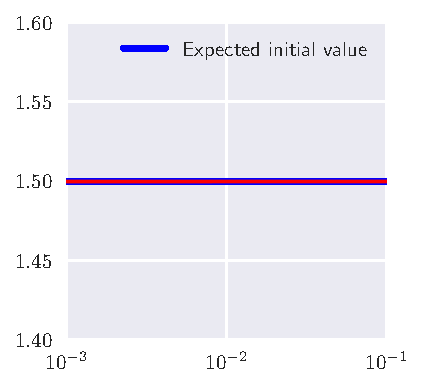
\includegraphics[width=1.\textwidth]{figures/risk_macroscopic.pdf}
    \caption{formula estimation}
  \end{subfigure}

  \caption{
    difference between two different strategies for estimating the risk in committee machine simulation.
    The two pictures are showing the same simulations and are zoomed on the very first part of the learning.
    There are 50 trajectories; we used 20000 samples for the estimation.
  }
  \label{fig:sampling_formula_risk}
\end{figure}

In Figure~\ref{fig:sampling_formula_risk} we show the difference between the last two strategies.
It's clear that the second one is preferable because the noise is reduced to 0, and the only difference
that appears in trajectories is caused by the stochasticity of the process.

\subsubsection{Finite size effect}
The key point of our analysis is the high dimensional limit; the derivation of 
deterministic differential equations are based on the limit \(d\to+\infty\).

When simulating a committee machine, we obviously can't use an infinite input layer dimension.
This introduces some finite-size effects. The simulations may not match exactly with the 
differential equations solution, but the difference becomes smaller and smaller by 
increasing the size used. 

This hypothetical problem has been a constant throughout this project,
although most of the time it has turned out not to be the cause of the discrepancies.
Many times we investigated the finite size effect, looking for a discrepancy scaling as
a power law (\(\propto d^\alpha\) for some \(\alpha\)), but we have not found any situation where
it was really affecting our results. Usually, \(d=10000\) was enough for our analysis; 
in the rest of this paper, we will not discuss this effect again assuming that
it is not relevant to what we are talking about, except where explicitly written.

% In Figure~\ref{fig:finite_size_example} we present an example of finite size effect;
% % todo: breve commento quando effettivamente metterai la figura.
% \begin{figure}
%   \begin{center}
%     \includegraphics[width=.7\textwidth]{example-image-duck}

%     \caption{
%       example of finite size effect. For details on how to interprete thi plot see Subsection~\ref{subsec:simulation_example}.
%     }
%     \label{fig:finite_size_example}
%   \end{center}
% \end{figure}

\subsection{Numerical solution of the differential equation}
The second ingredient needed for the numerical experiments of this work is a way to
solve the differential equations we derived in previous sections. Of course,
an explicit analytical solution is not feasible, given the complexity of the expressions;
we must therefore proceed with numerical integration techniques of differential equations. 

The most basic method for integrating a first-order differential equation is known
as \emph{Euler Method}, and it consists in discretizing the time in finite steps,
and compute the new value of the solution using the value at the previous step.
In our context, this becomes (let \(\delta t\) the time step)
\[
  \dod{\M{\left(t\right)}}{t} = \vec{\Psi}{\left(\vec{\Omega}\right)}
  \quad\xrightarrow{\text{Euler integration}}\quad
  \begin{cases}
    t^{(n)} = n \cdot \delta t \\
    \M^{(0)} = \M(0) \\
    \M^{(n)} = \vec{M}^{(n-1)} + \delta t\cdot\vec{\Psi}{\left(\vec{\Omega}^{(n-1)}\right)}
  \end{cases}\,.
\]
A completely analogous equation can be written for \(\Q\).

Of course, numerical integration introduces an error.
Since EM is a \emph{first-order method},
the error committed during the single step is proportional \(\delta t^2\).
Considering that the number of steps needed to reach a given time is inversely proportional
to the step size, the total error committed by this method of integration
is proportional to \(\delta t\).

For numerical experiments to be reliable, the error introduced by numerical integration
must be smaller (ideally negligible) than that due to switching from the stochastic process
to differential equations. Using the result of Theorem~\ref{thm:process_to_ode_goldt},
we get that the step size must satisfy
\[
  \delta t = \smallo{\frac{1}{\sqrt{d}}}\quad \text{ when }d\to+\infty.
\]
The usual choice for our numerical experiments is \(\delta t = \frac1d\);
this should ensure the negligibility condition respect the error of the Theorem.

\subsection{Example of a numerical experiment} \label{subsec:simulation_example}
\begin{figure}
  \begin{center}
    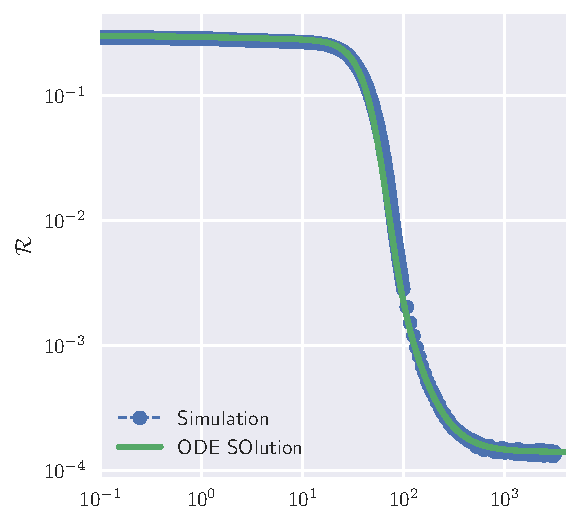
\includegraphics[width=.6\textwidth]{figures/simulation_examples_trajectory.pdf}

    \caption{
      the trajectory of both simulation and differential equations solutions in our example.
    }
    \label{fig:simulation_example_trajectory}
  \end{center}
\end{figure}
In this Section, we briefly present an experiment where we compare the simulation of committee machine training with the corresponding numerical simulation.
Although we do not present any results, we will use them to introduce some analysis tools that will be repeated in all future experiments.
We do not discuss the initial condition in this part since we will spend a lot of time on them in the next parts.

Let's start from the parameters used: \(d=1000, k=5, p=10, \gamma = 1., \Delta = \num{1e-3}, \delta t = \num{1e-3} \).
The only thing to be commented on here are the values of \(\Delta\) and \(\gamma/p\):
requiring the convergence of the process implies that they must not be too large;
we will derive precise inequalities in the sequel that will tell us exactly the maximum values that these two parameters can have.
For the moment, it is important to remember that they can be considered small enough to allow the second term of the equation for \(\Q\) to be considered at a lower order than the other terms of the ODEs.

Let's look at the plot of the risk through the process, in Figure~\ref{fig:simulation_example_trajectory}.
We use a logarithmic scale on both axes because we believe that's the best way to visualize what is going on in the process.
The simulation and solution trajectories of the differential equations match even though \(d\) is not very large;
this suggests that what has been exhibited so far is working. The simulated trajectory is subject to the noise introduced by the stochasticity of the training process,
so it will fluctuate around the trajectory defined by the solution of the differential equation. 
In the next Sections, we will often be interested in the transition between the initial flat phase and the onset of the fall (we call this transition ``drop from plateau'').
To make precise measurements in this area we will average several simulated trajectories in order to filter out the random part of the process.

To conclude, we present the analysis of the order parameter matrices, in Figure~\ref{fig:simulation_example_macroscopic}.
One important thing to say is that, given the symmetries, we discussed earlier,
it is sufficient to analyze the modulus of the matrix \(\M\). 
We see from the figure that even starting from a completely uncorrelated state,
the dynamics found both student-teacher correlations and student-student correlations.
Truth be told, we will not report this kind of graph for our later experiments mainly for reasons of space.
Nevertheless, the usage of plots such as these was very helpful in the analysis of the model.
Although in the future we will only show plots of the kind in Figure~\ref{fig:simulation_example_trajectory},
it was not the only tool used for analysis.
\begin{figure}
  \centering
  \begin{subfigure}{0.495\textwidth}
    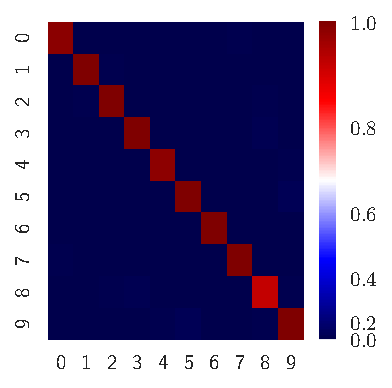
\includegraphics[width=1.\textwidth]{figures/simulation_examples_Q_start.pdf}
    \caption{\(\Q\) at start}
  \end{subfigure}
  \begin{subfigure}{0.495\textwidth}
    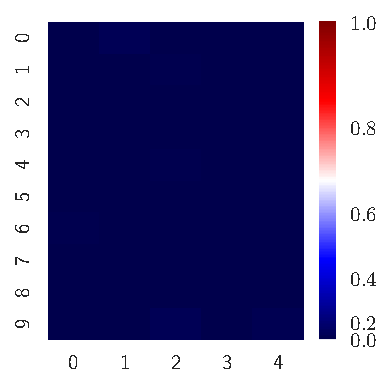
\includegraphics[width=1.\textwidth]{figures/simulation_examples_M_start.pdf}
    \caption{\(|\M|\) at start}
  \end{subfigure}
  \begin{subfigure}{0.495\textwidth}
    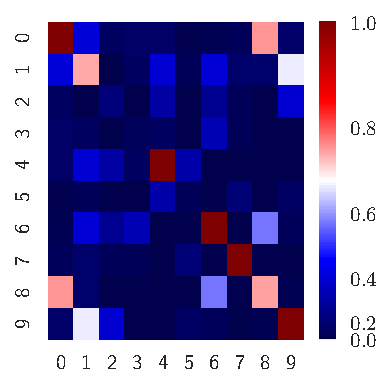
\includegraphics[width=1.\textwidth]{figures/simulation_examples_Q_end.pdf}
    \caption{\(\Q\) at end}
  \end{subfigure}
  \begin{subfigure}{0.495\textwidth}
    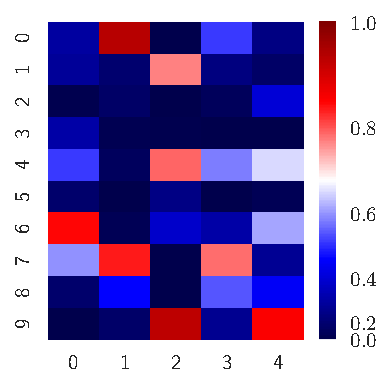
\includegraphics[width=1.\textwidth]{figures/simulation_examples_M_end.pdf}
    \caption{\(|\M|\) at end}
  \end{subfigure}

  \caption{
    order parameters matrix at the beginning and at the end of learning. 
  }
  \label{fig:simulation_example_macroscopic}
\end{figure}

Now that we know the tools we have available for analyzing an experiment, we can finally proceed with discussions about the content of the model.


\FloatBarrier
\section{Initial conditions}
In this Section, we present some considerations on the initialization of the student
and the teacher committee machines. As one may expect, the choice of the starting point 
can deeply affect the evolution of the training.
Moreover, we must always keep in mind that our ultimate goal is to give
an analytical estimate of the time required to learn the committee machine.
This forces us both to make a choice that produces analytically tractable equations
and to make a choice that is not too far removed from a real situation,
otherwise, the results would not be useful, despite being correct.

We initially present what was our first attempt to arrive at initial conditions suitable for our study.
Although it was not a fruitful choice,
we can still regard it as a toy model that serves as an introduction to the study of differential equations.
Next, we also report some other attempts, until we arrive at the final choice that we then used throughout our analysis.

\subsection{Symmetric initial condition} \label{subsec:symmetric_init}
Let's start by observing that form Equation~\eqref{eq:quadraticODE_M} it follows
that \(\M=0\) is a fixed point. This means that if we set completely non-overlapping
weights between student and teacher, then there is no learning at all, at least 
from the point of view of differential equations.
We would like to study the case where the teacher weights and the student's initial condition are uncorrelated,
and small perturbations around that. We introduce a framework where a parameter will
regulate the overlap, and the goal is doing perturbation around the fixed point.

The weights associated with a hidden node are vectors in \(\Real^d\), both for teacher and student.
Let \(\{\w^*_r\}_{r=1,\dots,k}\) the sets of weights of the teacher,
and \(V_T \coloneqq \Span\left[\{\w^*_r\}_{r=1,\dots,k}\right]\) the subspace generated by them.
We also assume these weights to be orthogonal. The initial weights for the student are chosen as
\[
    \w_j^0 = \frac{\varepsilon}{k} \sum_{r=1}^k \w^*_r + (1-\varepsilon) \w_j^S \quad
    \forall j\in [p],
\]
where the \(\w_j^S\) are orthogonal vectors of \(V_S \coloneqq (V_T)^\bot\),
the subspace of \(\Real^d\) orthogonal to the subspace of the teacher weights. 
The value of \(\varepsilon\) can vary between 0 and 1,
and it regulates the overlapping between student and teacher at the start.

We are using the following orthonormality conditions
\[
  \w^*_r \cdot \w^*_t = \rho_0d\delta_{rt}
  \qquad\text{and}\qquad
  \w_j^S\cdot\w_l^S=q_0d\delta_{jl},
\]
so the \emph{weights matrices} (\(\w_j \equiv [\W]_j\)) have orthogonal rows too.

Using all these assumptions, the computation of the order parameters leads to
\begin{align*}
  \left[\P\right]_{rt} &= \rho_0\delta_{rt}\\
  \left[\M^0\right]_{jr} &= \frac1d \w_j^0 \cdot \w^*_r = \frac{\rho_0\varepsilon}{k} \\
  \left[\Q^0\right]_{jl} &= \frac1d \w_j^0 \cdot \w^0_l = \frac1d
    \left(\frac{\varepsilon}{k} \sum_{r=1}^k \w^*_r + (1-\varepsilon) \w_j^S\right)\cdot
    \left(\frac{\varepsilon}{k} \sum_{t=1}^k \w^*_t + (1-\varepsilon) \w_l^S\right)\\
      &= \rho_0\frac{\varepsilon^2}{k} + q_0(1-\varepsilon)^2 \delta_{jl}
\end{align*}
An important feature of these initial conditions is that the order parameters are 
independent from \(d\), so the same differential equation solution can be used To
describe committee machines of different sizes.
Since what is really important is the rate between \(\rho_0\) and \(q_0\),
from now we will stick to the case \(\rho_0 = 1\).

\subsubsection{Fixed point with no overlap}
This case corresponds to null correlation, with \(\varepsilon=0\).
The initial conditions are 
\[\P = \I_k, \quad \M = 0 \quad \text{and}\quad \Q = q_0 \I_p.\]
As already pointed out, there is no evolution of \(\M\)
\[\M{(t)} = 0\quad \forall t\ge0,\]
and, through Equation~\eqref{eq:quadraticODE_Q},
this makes \(\Q\) always proportional to the identity matrix \(\Q{(t)} = q{(t)} \I_k\).
The important conclusion is that \(q(t)\) is the only variable that fully describes the evolution.
The equation Equation~\eqref{eq:quadraticODE_Q} becomes an explicit equation for \(q{(t)}\):
% ho rimosso tutti gli step perché non servono a niente. se proprio mettili in appendice
\begin{equation}\label{eq:eps0ODEforq}\begin{split}
    \dod{q{(t)}}{t} = \frac{4\gamma}{p}q{(t)}\Biggr\{&\underbrace{
        1 - \left(1+\frac2p\right) q{(t)}}_{\eqqcolon L{(q{(t)};p)}} \\
    &+\frac{\gamma}{p} \Biggr[\underbrace{
        \left(1+\frac2k+\Delta\right) - \Biggl(2 + \frac4p \Biggl)q{(t)} +
        \left(1+\frac6p+\frac{8}{p^2}\right)q^2{(t)}}_{\eqqcolon N{(q{(t)};p,k,\Delta)}}
    \Biggr]\Biggr\}.
\end{split}\end{equation}
We have introduced the two functions \(L\) and \(N\) in order to make the notation
lighter in the following part.

Since \(q(t)\) is descriptive of the whole process, we can write the population risk as its function
\[
  \risk{(t)} = \frac12\left[\left(1+\frac2k\right)-2q{(t)}+\left(1+\frac2p\right)q^2{(t)}\right].
\]
What it's really important about the last equation is that leads us to
\[
    \dod{\risk{(t)}}{t} = \left[\left(1+\frac2p\right)q{(t)}-1\right] \dod{q{(t)}}{t} = L{(q{(t)};p)} \dod{q{(t)}}{t},
\]
so stationary points of \(\od{q{(t)}}{t}\) are also stationary points of the risk itself, but the stability may be different.

Before continuing we show that \(L\) is always positive, regardless of the value of \(q\).
The function is a polynomial of the second degree,
so we have to show just that the (reduced) discriminant is less than 0
\[\begin{split}
  \left[-\left(1 + \frac2p \right)\right]^2 - \left(1+\frac6p+\frac{8}{p^2}\right)\left(1+\frac2k+\Delta\right) &<
  \left(1 + \frac2p \right)^2 - \left(1+\frac6p+\frac{8}{p^2}\right) \\
  &= 1 + \frac4p + \frac{4}{p^2} - 1-\frac6p-\frac{8}{p^2} 
  %=-(\frac2p+\frac{4}{p^2})
  <0.
\end{split}\]

We can now focus on the stationary and fixed points of the risk
since our ultimate goal is to have a description of its asymptotic behavior.
The first obvious fixed point is \(q=0\), but we are dealing only with positive values of \(q\),
so it's not interesting\footnote{
  We can show that if \(q{(0)}\) is positive, then we will never reach \(q=0\)
  by noticing that the time derivative of \(q\) is positive 
  in a right-neighborhood of \(q=0\).
}.
The second easy fixed point is the root of \(L{(q{(t)};p)}\):
\[q_{rm} \coloneqq \frac{1}{1+\frac2p} = \frac{p}{p+2}.\]
This corresponds to the minimum of the function \(\risk{(q)}\),
so it is not a real stationary point since the dynamic is governed by \(q\)
and this is not a fixed point for the \(q\) differential equation.

What really matters are the fixed points both for \(q\) and \(\risk\). 
Those are the roots of the equation obtained by imposing the left-hand-side 
of Equation~\eqref{eq:eps0ODEforq} equal to 0\footnote{
  We are assuming that solutions exist.
  If it not the case, then the problem is not interesting at all,
  since the risk will diverge independently from the value of \(q_0\).
}
\begin{equation}\begin{split}
  \displaystyle
  q_f^{1,2} &\coloneqq 
    \frac{p+2\gamma \mp
                \sqrt{\left[p+2\gamma\right]^2-
                      4\gamma p\frac{p+4}{p+2}
                        \left[1+\frac{\gamma}{p}\left(1+\frac2k+\Delta\right)\right]}}
                  {2\gamma\left(p+4\right)}p,
\end{split}\end{equation}

\begin{figure}
    \centering
    \begin{tikzpicture}[x=1.cm,y=1.cm,domain=0.:10.,range=-3.:5.]
      \filldraw [fill=Background,draw opacity=0.] (0,-3) rectangle (10.,5);
\draw[black, ->, thick] (0,0) -- (10,0) node[below] {\(q\)};
\draw[black, ->, thick] (0,-3) -- (0, 5) node[left] {\(\dod{q}{t}\)};

\draw (3,-0.15)--(3,0);
\draw (3.3,-0.15)--(3.3,0);
\draw (8,-0.15)--(8,0);

\draw[Blue, ultra thick] plot (\x,{0.4*(3-\x)});
\draw[Green, ultra thick] plot (\x,{0.1*(\x-3.3)*(\x-8)});

\draw[Red, dotted, thick] (3.3,0)--(3.3,1.5);
\draw[Red, dotted, thick] (3. ,0)--(3. ,1.5);
\draw[Red, |-|, ultra thick] (3. ,1.5) to node[Red,midway,above] {$\sim\BigO{\gamma}$} (3.3,1.5);

\node[above right] at (3.3,0) {$q_f^1$};
\node[below] at (3.,0) {$q_{rm}$};
\node[above] at (8,0) {$q_f^2$};
    \end{tikzpicture}
    \caption{
      the plot of the right-hand-side of Equation~\eqref{eq:eps0ODEforq}.
      The blue line is only the \(L\) contribution, while the green parabola is including also \(N\).
    }
    \label{fig:epsilon0stablepoints}
\end{figure}
To conclude our analysis, let us make a few considerations that will give us a clear picture
of how evolution works in this simple situation.
\begin{enumerate}
  \item \(q_f^1 < q_f^2\), by their definition;
  \item due to the fact that \(N{(q{(t)};p,k,\Delta)}\) is a positive function,
        the root of \(L{(q{(t)};p)}\) is always smaller than the full left-hand-side
        root in Equation~\eqref{eq:eps0ODEforq} (see also Figure~\ref{fig:epsilon0stablepoints} for a picture),
        so it holds\[q_{rm}<q_f^1 < q_f^2;\]
  \item As we already said, \(\risk{(q)}\) is a quadratic function and \(q_{rm}\) is the value of \(q\) that realize the minimum. Using previous step we can conclude
  \[\risk{(q_{rm})}<\risk{(q_f^1)} < \risk{(q_f^2)};\]
  \item We can show that \(q_f^1\) is a \emph{stable} point, while \(q_f^2\) is unstable (see Figure~\ref{fig:epsilon0stablepoints}).
  We can now infer the asymptotic behavior of the solution of the differential equation from the initial condition:
        \begin{itemize}
            \item \(0<q_0<q_f^2\): \(q{(t)}\to q_f^1\);
            \item \(q_0=q_f^2\): \(q{(t)}= q_f^2 \quad \forall t\);
            \item \(q_0>q_f^2\): \(q{(t)}\to +\infty\);
        \end{itemize}
        The interesting part comes from this initial value of \(q_0\):
        \[q_{rm}\le q_0<q_f^1 \quad \implies \quad \text{\(\risk{(t)}\) is a \textbf{strictly increasing} function}\]
        \[0\le q_0<q_{rm}     \quad \implies \quad \text{\(\risk{(t)}\) is a \textbf{non-monotonic} function}\]
  \item Let's look at the limit of small \(\gamma\):
        \[\lim_{\gamma\to0}q_f^1 = q_{rm} \quad\text{ and }\quad \lim_{\gamma\to0}q_f^2 = +\infty.\]
        This is in accordance with the common intuition that a smaller learning rate leads to better learning
        (even if talking about learning when there is no overlapping it's a little bit stretchy):
        we can go closer to the minimum and the interval where there is convergence is larger.
\end{enumerate}

We finally verified all our results from the study of differential equations with numerical experiments.
\begin{figure}
  \centering
  \begin{subfigure}{0.495\textwidth}
    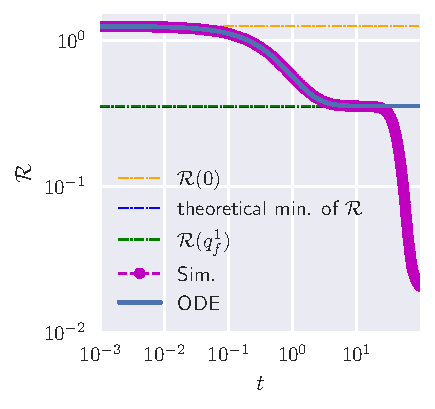
\includegraphics[width=1.\textwidth]{figures/example-eps0.pdf}
    \caption{global picture}
  \end{subfigure}
  \begin{subfigure}{0.495\textwidth}
    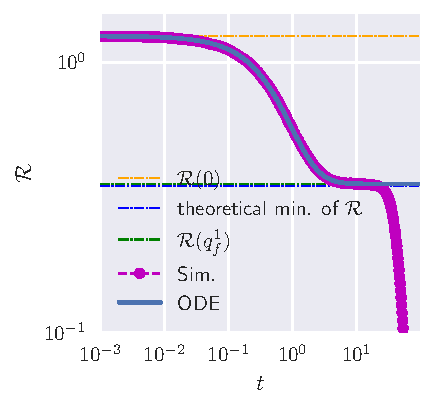
\includegraphics[width=1.\textwidth]{figures/example-eps0-zoomed.pdf}
    \caption{zoom}
  \end{subfigure}
  % Generated with: notebook epslion0
  \caption{
    example of a comparison between differential equations and simulations, with \(k=4\) and \(p=8\).
    The simulation and the analytic solutions match only in the first part.
    In Figure~(b) we zoom in on the region of the analytical prediction. We can see
    that the ODE solution converges to \(q_f^1\) and the theoretical risk minimum at \(q_{rm}\).
  }
  \label{fig:example-eps0}
\end{figure}
In Figure~\ref{fig:example-eps0} we show an example of a comparison between differential equations and simulations.
The first thing that stands out is that the simulations actually learn the teacher.
This happens because learning is a stochastic process, and the noise introduced
by the randomness of the SGD breaks the symmetry forced by the initial conditions.
On the other hand, the differential equations are deterministic, and their structure
is able to maintain the initial symmetry; the analytic solution gets stuck in the 
\emph{second plateau}. The only dynamics the ODE are able to catch in this case is 
the \emph{norm learning}: the weights of the student are changing their norm to adapt 
to the teacher, but their directions instead are not varying.

In the end, this section studied some initial conditions that do not bring out any kind of interesting learning.
In any case, the study of this simple toy model was useful to better understand the behavior of the dynamics of this strange activation function.
Finally, these particular initial conditions will be taken up in Chapter \ref{chap:stochasticity}.

\subsubsection{Overlapped intial condition}
We now generalize the study to the case \(\varepsilon\neq0\).
The initial conditions can be written as
\[\begin{split}
    \P &= \I_k,\\
    \M{(0)} &= \frac{\varepsilon}{k}\J_{p,k},\\
    \Q{(0)} &= \frac{\varepsilon^2}{k}\J_{p} + q_0(1-\varepsilon)^2\I_{p}.\\
\end{split}\]
We now show that \(\M\) and \(\Q\) stay in the same form through evolution, so we can write
\[\begin{split}
    \M{(t)} &= m{(t)} \J_{p,k} \\
    \Q{(t)} &= s{(t)} \J_{p} + q{(t)}\I_{p} \\
\end{split}\]
and the problem is completely described by a system of three coupled differential equations.
In order to prove this, it's sufficient the following identities
\[
    \I_d^n=\I_d, \quad \J_{d,f}^n = f^{n-1}\J_{d,f}, \quad \J_{d,f}\I_f = \J_{d,f}, \quad\text{and}\quad
    \J_{d,f} \J_{g,f}^\top = f \J_{d,g}.
\]
They are proof that the set \(\{\I,\J\}\) is closed under the operations that appear in differential equations.

The full derivation for the differential equations of \(m{(t)}\), \(q{(t)}\) and \(s{(t)}\) is 
omitted, since it's not particularly interesting. 

We avoided doing a careful study like the one in the previous section for the system of differential equations.
These initial conditions are not sufficiently general for a complete study of the learning process:
they still contain a symmetry that is preserved by the ODEs but broken from the 
stochasticity in the simulation. 
\begin{figure}
  \centering
  \begin{subfigure}{0.495\textwidth}
    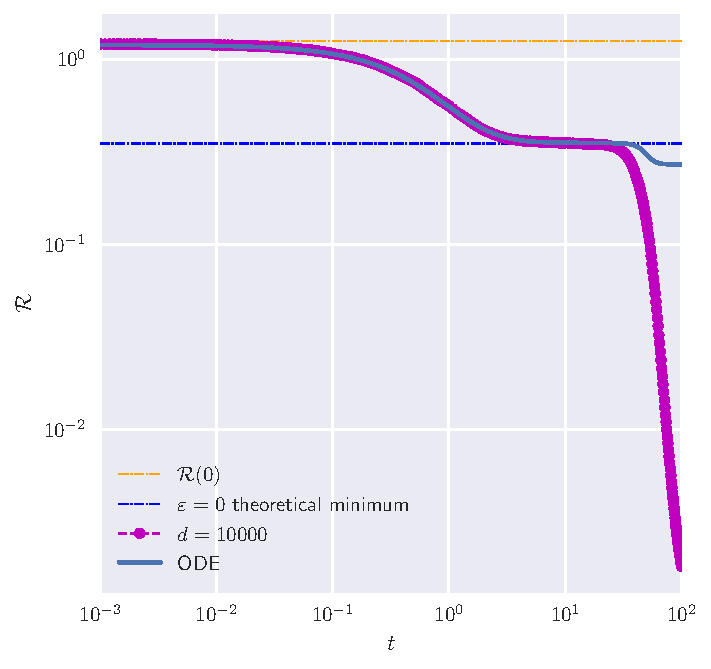
\includegraphics[width=1.\textwidth]{figures/example-small-eps.pdf}
    \caption{global picture}
  \end{subfigure}
  \begin{subfigure}{0.495\textwidth}
    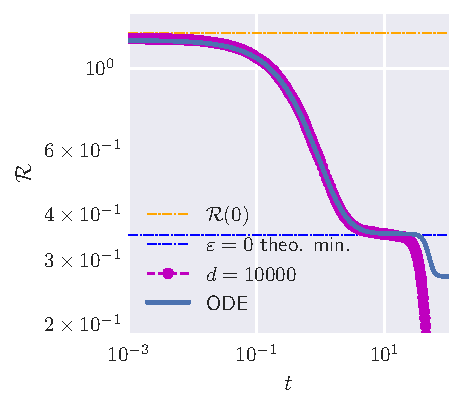
\includegraphics[width=1.\textwidth]{figures/example-small-eps-zoom.pdf}
    \caption{zoom}
  \end{subfigure}
  % Generated with: notebook small-epsilon
  \caption{
    example of a comparison between differential equations and simulations, with \(k=4\), \(p=8\) and \(\varepsilon=0.01\).
    The simulation and the analytic solutions match only in the first part.
    In Figure~(b) we zoom on the region of the analytical prediction.
    As in the previous case, the differential equations solution gets stuck in symmetry,
    while the simulation learns completely. The ``drop from the plateau'' happens before 
    the ODEs solution reaches its final value. 
  }
  \label{fig:example-small-eps}
\end{figure}

In Figure~\ref{fig:example-small-eps} we show an example of comparisons between simulation
and differential equation solution. The ODEs are now able to catch 2 different phases of 
the learning: the norm learning and the \emph{linear learning}. In the analytical dynamic,
they are clearly separated: the first part perfectly replicates what we saw in the previous section;
in the second part linear learning occurs, that is, each hidden neuron learns the same thing,
and the student's committee machine behaves as if \(p=1\).
This is evident from the fact that \(\M\) is proportional to \(\J\):
each hidden neuron is on average a copy of the others, they all learn the same weights.
In Figure~\ref{fig:pictorial-symmetric-learning} we present a schematic view of the different phases of the learning,
using symmetric initial conditions.
\begin{figure}
  \centering
  \begin{tikzpicture}[
    x=1.cm,
    y=1.cm
  ]
    \filldraw [fill=Background,draw opacity=0.] (0,0) rectangle (10.,9.);
\draw[black, ->, thick] (0,0) -- (10,0) node[below] {\(\log t\)};
\draw[black, ->, thick] (0,0) -- (0, 9) node[left] {\(\log\mathcal{R}\)};

\draw[
  line width=1.5mm,
  Red,
  looseness=1.1
] (0,8) to[out=0, in=180]
  (1.0,8) to[out=0, in=180]
  (2., 7) to[out=0, in=180] 
  (10, 7);

\draw[
  line width=1.mm,
  Blue,
  looseness=1.1
] (0,8) to[out=0, in=180]
  (1.0,8) to[out=0, in=180]
  (2., 7) to[out=0, in=180] 
  (4., 7) to[out=0, in=180]
  (5., 5) to[out=0, in=180]
  (10, 5);

\draw[
  line width=0.5mm,
  Green,
  looseness=1.1
] (0,8) to[out=0, in=180]
  (1.0,8) to[out=0, in=180]
  (2., 7) to[out=0, in=180] 
  (4., 7) to[out=0, in=180]
  (5., 5) to[out=0, in=180]
  (6., 5) to[out=0, in=180]
  (8., 1.5) to[out=0, in=180]
  (10., 1.5);

\node[right] at (1.5,7.55) {norm learning};
\node[left] at (4.5,6.) {linear learning};
\node[left] at (7.,3.25) {specialization};

\node[Red, above] at (9,7.05) {\(\varepsilon=0\)};
\node[Blue, above] at (9,5.05) {\(\varepsilon>0\)};
\node[Green, above] at (8.8,1.55) {\(\text{no symmetry}\)};

  \end{tikzpicture}
  
  \caption{
    pictorial representation of the different phases of learning for symmetric initial conditions.
  }
  \label{fig:pictorial-symmetric-learning}
\end{figure}

As already mentioned, simulations break this symmetry, and they do so before linear learning.
To be able to see the second plateau even in simulations would require using a much larger value of \(d\),
but this is not computationally feasible. 

We have empirically observed that in typical situations the various stages of learning are not really distinct and occur simultaneously,
so we decided to abandon symmetric initial conditions from here on,
in order to look for others that would suit us better.


\subsection{Random Initial condition} \label{subsec:random-initial-conditions}
In the last section, we have essentially come to the conclusion that
choosing initial conditions with some structure is convenient
because it simplifies the differential equations,
but it also introduces artificial symmetries that prevent the study of the complete problem.
We must therefore explore new possibilities to find ways to analyze the process of learning.

We decide to try some random initial conditions, to be sure that no symmetry is still present,
but at the same time use the high-dimensional limit to have statistical control on the 
order parameters. Moreover, we focus on the \emph{phase retrieval} case at first 
and then generalize once good initial conditions are found.
Accordingly, we will use the notation and the equations introduced in Section~\ref{subsec:phase_retrieval}.

We start our derivation by choosing both \(\vec{w}\) and \(\vec{w}^*\) to be independent normal
vectors with unit variance
\[
  w_{i}, w^*_{i} \sim \gauss{(0,1)}\quad\text{and all indipendent.}
\]
It follows that the order parameters are random variables too, distributed as
\emph{chi-squared} distribution
\[
  q(0),\rho \sim \frac{\chi^2_d}{d}
\]
and consequently 
\[
  \E\left[q(0)\right] = \E\left[\rho\right] = 1 \quad\text{and}\quad
  \Var\left[q(0)\right] = \Var\left[\rho\right] = \frac{2}{d}.
\]
The distribution of \(m{(0)}\) is not as simple as the previous two but can be derived exactly.
In our analysis it's sufficient to have the expected value and the variance, then use the 
\emph{central limit theorem} since we are interested in the high-dimensional limit.
Denoting \(X,Y\) two independent unitary normal variables, we can compute
\[\begin{split}
  \E\left[m{(0)}\right] =& \E\left[\frac{\sum_{i=1}^d w_iw^*_i}{d}\right] = \E\left[XY\right] = 0, \\
  \Var\left[m{(0)}\right] =& \Var\left[\frac{\sum_{i=1}^d w_iw^*_i}{d}\right]
    = \frac{1}{d^2}\sum_{i=1}^d \Var\left[XY\right] = \frac{1}{d}.
\end{split}\]
What emerges from these initial conditions is that, in the high-dimensional limit,
\(\vec{w}\) and \(\vec{w}^*\) are approximately two orthogonal vectors on the hemisphere of radius \(\sqrt{d}\).

The natural thing to do now is to replace these combined initial conditions with Equations~\eqref{eq:phase_retrieval},
with the aim of deriving approximate dynamics for the first part of learning
and to derive from it an analytical approximation of the learning time.
The problem is that is not clear how to do the approximation: an experiment reported in Figure~\ref{fig:unconstraned-random-example},
shows that \(q\) is varying considerably even before the learning starts.
This makes impossible all low-order expansions of differential equations and,
ultimately, analytical analysis of the phenomenon.
Nevertheless, in Figure~\ref{fig:unconstraned-random-m-exit-time} we show how an analysis of the simulations seems to suggest
a logarithmic trend in learning time as size changes. It is a crude numerical estimation of the behavior of the committee machine,
but it gives us a first idea of what is going on. To conclude, the behavior emerged from this analysis
is in accordance with what we may expect from past literature\cite{arous2021online}.
\begin{figure}
  \centering
  \begin{subfigure}{0.495\textwidth}
    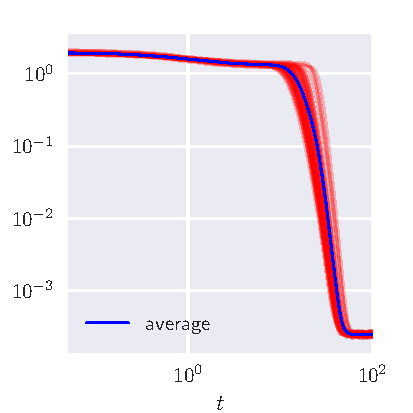
\includegraphics[width=1.\textwidth]{figures/unconstraned-phase-retrieval-risk.pdf}
    \caption{risk \(\mathcal{R}\)}
  \end{subfigure}
  \begin{subfigure}{0.495\textwidth}
    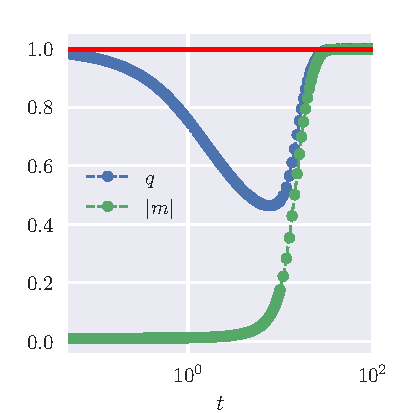
\includegraphics[width=1.\textwidth]{figures/unconstraned-phase-retrieval-qm.pdf}
    \caption{\(q\) and \(|m|\)}
  \end{subfigure}
  % Generated with: random-orthonormal-k=1
  \caption{
    example of simulation with random initial condition and \(d=10000\).\\
    In Figure~(a) we can see many different possible trajectories (red) and their average (blue).
    In Figure~(b) we plot the average of \(q\) and \(|m|\) over different trajectories.
    It's clear that the order parameter \(q\) is evolving considerably before the drop from initial
    plateau, so these initial conditions are not suitable for our goal.
  }
  \label{fig:unconstraned-random-example}
\end{figure}
\begin{figure}
  \centering
  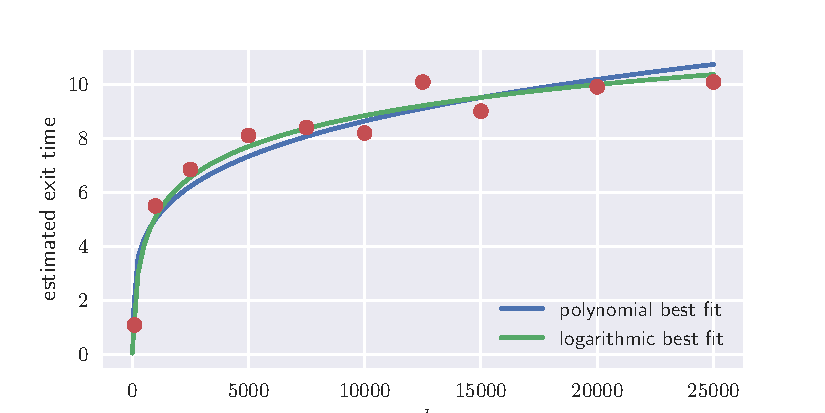
\includegraphics[width=\textwidth]{figures/unconstraned-phase-retrieval-exittimes.pdf}
  % Generated with: random-orthonormal-k=1
  \caption{
    plot of the \(|m|\) simulated exit time, and the corresponding best-fit curves.\\
    The exit time is estimated by measuring the time when the function \(m(t)\), averaged over many trajectories,
    crosses the threshold value \(0.1\).
    Looking at the figure, it is possible to convince oneself that 
    the logarithmic best fit better traces the behavior that emerged from the simulations. 
  }
  \label{fig:unconstraned-random-m-exit-time} 
\end{figure}
\FloatBarrier

In order to make the expansion possible, we have to set \(q(0)\) to be close to 0;
in other words, the norm of \(\vec{w}\) should be nearly null.
Obviously, we can't start exactly with \(\vec{w}=\vec{0}\), because it's a fixed point
of the differential equations dynamics.
Our goal can be achivied by intializing the student with \(w_{i}\sim\gauss(0,\sigma^2)\),
with \(\sigma^2\ll1\).
Recomputing the expected value above that are affected by this scaling of \(\vec{w}\), we get 
\[
  \E\left[q(0)\right] = \sigma^2\,, \quad
  \Var\left[q(0)\right] = \frac{2\sigma^2}{d}\quad\text{and}\quad
  \Var\left[m{(0)}\right] = \frac{\sigma}{d}. 
\]
The difference between these initial conditions and the previous one is illustrated in Figure~\ref{fig:pictorial-unconstrainted-phase-retrieval} .
\begin{figure}
  \centering
  \begin{tikzpicture}  
    % Credits to Nica 

% Sfera
\draw[turquoise, thick] (5,0) arc (0:180:5);

\fill[turquoise!33] (5,0) arc (0:180:5);

\draw[turquoise, thick, dashed] (0,0) ellipse (5 and 1.5);
\fill[turquoise!33] (0,0) ellipse (5 and 1.5);

% Vettori
\draw[black, ->] (0,0) -- (0,5) node[midway,right] {\(\vec{w}^*\)};

\draw[orange, ->] (0,0) -- (4,0.9) node[midway,above] {\(\vec{w}\)};

\draw[red, ->] (0,0) -- (-.8,0) node[midway,above] {\(\sigma^2\)};

\draw[loosely dashdotted, orange] (0,5) -- (4, 0.9);
\draw[gray] (0,0) -- (4, -0.9) node[midway,below]{$\sqrt{d}$};
\draw[loosely dashdotted, red] (0,5) -- (-.8,0);
  \end{tikzpicture}
  \caption{
    a pictorial plot of the phase retrieval weights with these initial conditions.
    The teacher weight, up to rotation, it's the pole vector in a semisphere 
    (here represented in 3D, but in the real case is \(d\)-dimensional);
    we can limit ourselves to analyzing only a hemisphere since the \(\vec{w}\to-\vec{w}\) symmetry applies.\\
    The two colored vectors represent the student's initial conditions, approximately orthogonal to the teacher vector. 
    The dashed lines are tentatives paths of the student vectors during the learning: starting close to the origin
    should make the norm grow towards~1, without any non-monotonic behavior.
  }
  \label{fig:pictorial-unconstrainted-phase-retrieval} 
\end{figure}
First of all, we observe that the sign of \(m(t)\) is not important for monitoring the learning. Therefore, the quantity
we are really interested in as initial condition is \(|m{(0)}|\). Using the \emph{half-normal distribution} properties\cite{enwiki:halfnormaldistribution},
we can compute
\[
  \E{\left[|m{(0)}|\right]} = \sqrt{\frac{2}{\pi d}}\sigma.
\]
We can now proceed to do a linear expansion of Equations~\eqref{eq:phase_retrieval} around the starting point
\begin{subequations}\begin{align}
  \dod{|m{(t)}|}{t} &= 6 \gamma |m{(t)}|\\
  \label{eq:sigma_phase_retrieval_q}
  \dod{q{(t)}}{t} &= \left(4 \gamma + 12 \gamma^2 + 4\Delta\right) q{(t)}
\end{align}\end{subequations}
where we transformed the equation for \(m(t)\) in the one for the modolus,
and kept only the linear terms of the equations\footnote{
  The expansion is not rigorous, since \(m(t)\) and \(q(t)\) are ``small'' for different reason.
  In order to do a proper derivation, we should keep track of different orders in different variables.
  The purpose of this part is to give an insight into what we will be doing in the next chapters.
}; we have also set \(\rho=1\), following what was computed above.
Using the expected values computed above as starting values, we get this evolution for the order parameters
\[
  |m(t)| = \exp{\left[6\gamma t\right]}\sqrt{\frac{2}{\pi d}}\sigma \quad\text{and}\quad
  q(t) = \exp{\left[\left(4 \gamma + 12 \gamma^2 + 4\Delta\right)t\right]}\sigma^2.
\]
We stress again that this evolution are approximating the real one only when \(m(t),q(t)\ll1\).
Despite this, we can still estimate exit times, provided the thresholds used are also small.
Let \(T\) the value of the threshold, valid both for \(m\) and \(q\), then the exit times are
\begin{equation}
  t_\text{ex}^{(m)} = \frac{\log{\left[\frac{T}{\sigma}\sqrt{\frac{\pi d}{2}}\right]}}{6\gamma} \quad\text{and}\quad
  t_\text{ex}^{(q)} = \frac{\log{\left[\frac{T}{\sigma^2}\right]}}{4 \gamma + 12 \gamma^2 + 4\Delta}.
\end{equation}
The thing to note is that \(t_\text{ex}^{(q)}\) does not depend on \(d\).
To make the result more accurate, we can make a correction to Equation~\eqref{eq:sigma_phase_retrieval_q}
and obtain a new form for the time evolution of \(q(t)\) that includes also the effect of \(m(t)\)
\[
  \dod{q{(t)}}{t} = \left(4 \gamma + 12 \gamma^2 + 4\Delta\right) q{(t)} + \left(8\gamma+48\gamma^2\right)m^2{(t)}.
\]
We can plug in the solution we found for \(|m(t)|\) and solve the equation to obtain\footnote{
  We are assuming that only \(m(t)\) can influence \(q(t)\) and that the reverse does not happen.
  This is not formally correct, but it is what happens in practice for reasonable choices of initial parameters.
}
\[\begin{split}
  q{(t)} = \frac{1}{f_{\gamma,\Delta}}\Bigg\{&\sigma^2\left[(8\gamma-12\gamma^2-4\Delta)-\left(8\gamma+48\gamma^2\right)\frac{2}{\pi d}\right]\exp\left[\left(4 \gamma + 12 \gamma^2 + 4\Delta\right)t\right]\\
          &+\left(8\gamma+48\gamma^2\right)\frac{2}{\pi d}\sigma^2 \exp\left[12\gamma t\right]\Bigg\},
\end{split}\]
where \(f_{\gamma,\Delta} \coloneqq 8\gamma-12\gamma^2-4\Delta\).
The evolution of \(q\) is contributed by two exponential;
it is not possible to derive an exact expression of the exit time,
but we can make the approximation that the two exponentials contribute separately
and thus take the minimum between the two possible times:
\[
  t_\text{ex}^{(q)} = \min\left(\frac{1}{4 \gamma + 12 \gamma^2 + 4\Delta}\log{\left[\frac{T}{\sigma^2}\right]},
                                \frac{1}{12\gamma}\log{\left[\frac{T}{\sigma^2}\frac{\pi d}{2}\frac{8\gamma-12\gamma^2-4\Delta}{8\gamma+48\gamma^2}\right]}\right),
\]
where we also dropped some subleading terms in \(d\).

Figure~\ref{fig:sigma-phase-retrieval-exittimes} shows a comparison between what is predicted by the formulas
and what is actually measured by doing numerical experiments.
\begin{figure}
  \centering
  \begin{subfigure}{0.495\textwidth}
    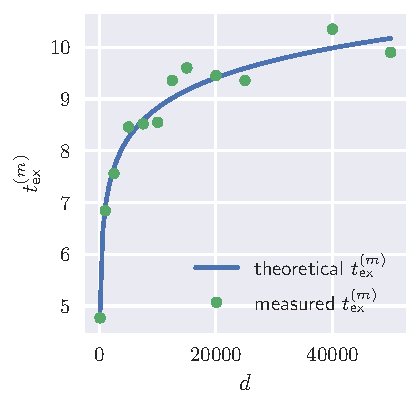
\includegraphics[width=1.\textwidth]{figures/sigma-phase-retrieval-mexit.pdf}
    \caption{exit time for \(|m|\)}
  \end{subfigure}
  \begin{subfigure}{0.495\textwidth}
    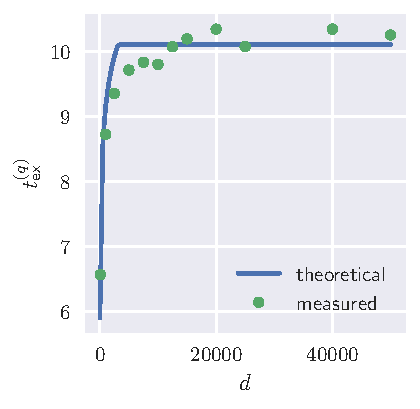
\includegraphics[width=1.\textwidth]{figures/sigma-phase-retrieval-qexit.pdf}
    \caption{exit time for \(q\)}
  \end{subfigure}
  % Generated with: random-orthonormal-k=1
  \caption{
    comparison between the exit time obtained from differential equations and the one measured in simulations. \\
    In the simulations we used \(\gamma=\num{0.1}, \sigma=\num{0.01}, T=\num{0.02}\).
  }
  \label{fig:sigma-phase-retrieval-exittimes}
\end{figure}
The predictions for \(t_\text{ex}^{(m)}\) are quite accurate,
while the ones for \(t_\text{ex}^{(q)}\) are only partially correct.
We can clearly see that our formula fails to predict the exit time in the transition
between the two regimes; probably the assumption that the two exponentials can be treated separately does not hold.
For large \(d\) the \(q\)-exit-time does not depend on \(d\) and the theoretical prediction seems correct.

The results obtained in this section, although not exhaustive,
provide an outline for what we are going to do in the next chapters of this paper.
The idea of random initial conditions combined with an expansion of differential equations seems promising,
but it has not yet led to the desired results.
The introduction of \(\sigma\) indeed made the expansion possible,
but it did not solve all the problems related to the norm of the \(\vec{w}\) vector;
it simply shifted the problem. 
The flat part in \(t_\text{ex}^{(q)}\)'s plot is a manifestation of the fact that the learning (linear or specialization) of the committee machine is still not being analyzed directly.
Achieving this goal will require a paradigm shift, as we will see in the next chapter.

  \chapter{Spherical Constraint}
In this chapter we investigate the problem in a different paradigm than what we did before.
With the aim of explicitly discriminating between norm learning and other learning steps,
we fix the value of the norm of weights at each step of the gradient descent.
A new dynamic emerges, from which, through the study of the associated differential equations,
we will derive some interesting properties of the process.

In the first section of the chapter we will give a mathematical defiition of the dynamics we will use and derive the associated differential equations.
In the next parts we will apply what we found to phase retrivial, and then generalize step by step to the case of a generic committee machine.


\section{Constrainted dynamics and differential equations}
In this section we adapt the dynamics, both for gradient descent and differential equations, to the new spherical constraint.
The derivation we present it's general and it does not assume anything on the activation function;
the results we will present will therefore be valid for any choice of activation function.
We will use the notation introduced in Chapter~\ref{chap:context}.

We start by assuming that all the weights we deal with belong to the sphere in \(d\) dimensions of radius \(\sqrt{d}\)
\[
  \vec{w}^\nu_j, \vec{w}^*_r \in S^{d-1}{\left(\sqrt{d}\right)}.
\]
The choice of radius, and hence normalization, follows from the fact that we want
the macroscopic variables to be of order 1 even in the high-dimensional limit.

In order to make valid this assumption, we have to force the norm of the student's weights to be
exactly \(\sqrt{d}\) at every step of the process. We modify the update rule as follows
\[ \w^{\nu+1}_j =\frac{\w^{\nu}_j - \gamma \nabla_{\w_j}{\loss}}{\left\|\w^{\nu}_j - \gamma \nabla_{\w_j}{\loss}\right\|}\sqrt{d}.\]
%todo: parla un po' delle varie possibilitá di gradiente e del perché alla fine abbiamo scelto questa.
We might naively think that it may suffice to take the component of the gradient tangent to the hypersphere,
and move in that direction using therefore as an update rule
\[
  \w^{\nu+1}_j = \w^{\nu}_j - \gamma \left[
    \nabla_{\w_j}{\loss} - \left(\frac{\w^{\nu}_j}{\sqrt{d}}\cdot\nabla_{\w_j}{\loss}\right)\frac{\w^{\nu}_j}{\sqrt{d}}
  \right].
\]
Unfortunately, this is not enough to maintain the spherical constraint on the weights.
The process we are analyzing is discrete, and it is the finite learning rate that causes the weights to lose the required normalization.
In order to use the gradient tangent to the surface we must take the limit \(\gamma\to0\).
This regime is known as \emph{gradient flow} and has already been used to study two-layers neural networks (in example \cite{chizat2018global}).
However, it is not what we want to study, so we will continue with the first update rule we proposed.

The update rule can be directly used for simulating the training process of a committee
machine, but it requires some work before it can be used for deriving some differential equations.
In particular, we want to find it's expansion for \(d\to+\infty\), keeping only leading orders terms.
Before proceeding to the expansion, we analize the order of single terms,
rembering the quantities we are dealing with are random variables.

We recall that the gradient is vector of random variables because of its dependence on \(\vec{x}^\nu\).
To be precise, also the displacement \(\dsp\) is a random variable, but the order of its value does not scale with \(d\),
so for our purpose it does not count. The gradient of the loss is given by
\[\nabla_{\w_j}{\loss} = -\frac{1}{p}\dsp^\nu_j \frac{\vec{x}^\nu}{\sqrt{d}}.\]
We can show that both the norm and the scalar product with a weight vector are order 1
\[\begin{split}
  \left\|\nabla_{\w_j}{\loss}\right\|^2 \sim&
    \frac{\dsp^2_j}{p^2} \frac{\sum_{i=1}^d \left(x^\nu_i\right)^2}{d}\sim
    \frac{\dsp^2_j}{p^2}\frac{\chi^2_d}{d} = \BigO{1},\\
  \w_j\cdot\nabla_{\w_l}{\loss} \sim&
    -\frac{\dsp_l}{p}\sum_{a=1}^d\frac{w_{j,a}}{\sqrt{d}}\gauss{(0,1)} \sim
    -\frac{\dsp_l}{p^2}\gauss{\left(0,\sum_{a=1}^d\frac{w^2_{j,a}}{d}\right)} \sim
    -\frac{\dsp_l}{p^2}\gauss{\left(0,1\right)}= \BigO{1}.
\end{split}\]

We are now ready to write the update rule expansion.
 Let's start by computing the the normalization factor
\[\begin{split}
  \frac{1}{\left\|\w^{\nu}_j - \gamma \nabla_{\w_j}{\loss}\right\|} =&
    \left[\left(\w^{\nu}_j - \gamma \nabla_{\w_j}{\loss}\right)\cdot\left(\w^{\nu}_j - \gamma \nabla_{\w_j}{\loss}\right)\right]^{-\frac12} \\
    =&\left[\left\|\w^{\nu}_j\right\|^2 - 2\gamma\w^{\nu}_j\cdot \nabla_{\w_j}{\loss}+\gamma^2\left\|\nabla_{\w_j}{\loss}\right\|^2\right]^{-\frac12} \\
    =&\frac{1}{\sqrt{d}}\left[1- \frac1d\left(2\gamma\w^{\nu}_j\cdot \nabla_{\w_j}{\loss}-\gamma^2\left\|\nabla_{\w_j}{\loss}\right\|^2\right)\right]^{-\frac12} \\
    =&\frac{1}{\sqrt{d}}\left[1+ \frac{1}{2d}\left(2\gamma\w^{\nu}_j\cdot \nabla_{\w_j}{\loss}-\gamma^2\left\|\nabla_{\w_j}{\loss}\right\|^2\right)+\smallo{d^{-1}}\right]
\end{split}\]
We can now plug this expansion back in the original update rule
\[
  \w^{\nu+1}_j =\left(\w^{\nu}_j - \gamma \nabla_{\w_j}{\loss}\right)\left[1+ \frac{1}{2d}\left(2\gamma\w^{\nu}_j\cdot \nabla_{\w_j}{\loss}-\gamma^2\left\|\nabla_{\w_j}{\loss}\right\|^2\right)+\smallo{d^{-1}}\right]\sqrt{d}.
\]
Let us notice that if we keep only leading terms in the learning rate we obtain 
the naive update rule we discussed above. 
This is consistent with what we have said about the gradient flow regime. 

We are ready to go over the steps that take us from the update rule on vector weights
to those on order parameters. We report by way of example the steps performed for \(\M\);
the accounts for \(\Q\) are similar, just a bit more tedious.
\[\begin{split}
  \left[\M^{\nu+1}\right]_{jr} &= \frac{\w^{\nu+1}_j\cdot\w_r^*}{d} \\
    &= \left(\left[\M^{\nu}\right]_{jr} - \frac{\gamma\w_r^*\cdot\nabla_{\w_l}{\loss}}{d}\right)\left[1+ \frac{1}{2d}\left(2\gamma\w^{\nu}_j\cdot \nabla_{\w_j}{\loss}-\gamma^2\left\|\nabla_{\w_j}{\loss}\right\|^2\right)+\smallo{d^{-1}}\right]\\
    &= \left[\M^{\nu}\right]_{jr} - \frac{\gamma\w_r^*\cdot\nabla_{\w_l}{\loss}}{d} + \frac{\left[\M^{\nu}\right]_{jr}}{2d}\left(2\gamma\w^{\nu}_j\cdot \nabla_{\w_j}{\loss}-\gamma^2\left\|\nabla_{\w_j}{\loss}\right\|^2\right)+\smallo{d^{-1}} \\
    &= \left[\M^{\nu}\right]_{jr} +\frac{1}{d}\left[
      \frac{\gamma}{p} \lf^*_r\dsp^\nu_j -
      \frac{\left[\M^{\nu}\right]_{jr}}{2}\left(2\frac{\gamma}{p}\dsp^\nu_j\lf^\nu_j + \frac{\gamma^2}{p^2} {\dsp^\nu_j}^2\right)
    \right] + \smallo{d^{-1}}.
\end{split}\]
We can now take the limit \(d\to+\infty\), claiming that the Theorem~\ref{thm:process_to_ode_goldt} is still valid.
It's not hard to belive that it is, since in the right-hand-side we have expression of the same kind
as those in the original version of the theorem; we will make the similarity explicit in a moment.
Indeed, if the hypothesis are met, than we have the same ``concentarting to mean''behaviour we have already encutered.
The differential equation that describe the evolution of \(\M\) is
\[
  \dod{\left[\M{\left(t\right)}\right]_{jr}}{t} =\E_{\vec{\lf},\vec{\lf^* \sim \gauss{(0,\vec{\Omega}{(t)})}}}{\left[\frac{\gamma}{p} \dsp_j \lf_r^* - \frac{\left[\M{\left(t\right)}\right]_{jr}}{2}\left(2\frac{\gamma}{p}\dsp^\nu_j\lf^\nu_j + \frac{\gamma^2}{p^2} {\dsp^\nu_j}^2\right)\right]};
\]
Using the definitions introduced in Equations~\eqref{eq:genericODEforM}~and~\eqref{eq:genericODEforQ} we can write the equation in a nicer form
\begin{equation} \label{eq:genericsphericalM}
  \dod{\left[\M{\left(t\right)}\right]_{jr}}{t} = \Psi_{jr}{(\vec{\Omega})} - \frac{\left[\M{\left(t\right)}\right]_{jr}}{2}\Phi_{jj}{(\vec{\Omega})}.
\end{equation}
Essentially, the spherical constraint can be imposed by using a term proportional to the unconstrainted \(\Q\) update.

Without reporting all the calculations, we can write an analougus differential equation for \(\Q\) evolution
\begin{equation} \label{eq:genericsphericalQ}
  \dod{\left[\Q{\left(t\right)}\right]_{jl}}{t} = \Phi_{jl}{(\vec{\Omega})} - \frac{\left[\Q{\left(t\right)}\right]_{jl}}{2}\left(\Phi_{jj}{(\vec{\Omega})}+\Phi_{ll}{(\vec{\Omega})}\right).
\end{equation}
Note that \(\dod{\left[\Q{\left(t\right)}\right]_{jj}}{t}=0\) if \(\left[\Q{\left(t\right)}\right]_{jj}=1\),
as it should be since the norm of spherical vectors must not change.

The two equations we derived are valid for any activation function; we can find an explicit form for the squared activation using
the expression of \(\Phi\) and \(\Psi\) we wrote in Equations~\eqref{eq:quadraticODEs}.
In Figure~\ref{fig:example-spherical} we present an example of the new dynamic
with a comparsion to the unconstrained one.
\begin{figure}
  \centering
  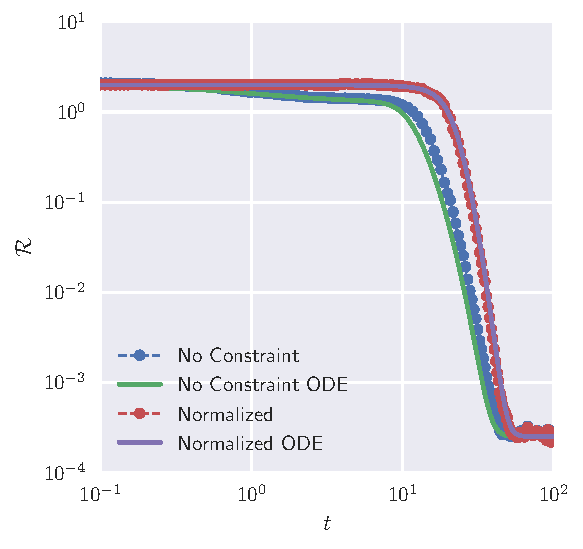
\includegraphics[width=0.7\textwidth]{figures/example-spherical.pdf}
  \caption{
    comparsion between spherical constrainted and unconstrained dynamics starting from the same intial condition.
    As we might expect in unconstrained dynamics less time is required for learning since
    there are no constraints on the gradient descent path.
    Since the simulation is not an average over several trajectories,
    it is also possible to observe the noise introduced by the stochasticity of the process;
    the constrained dynamics is less subject to noise and consequently the solution of the differential equations
    better approximates the single trajectory of the simulation.
  }
  \label{fig:example-spherical}
\end{figure}

\subsection{Initial conditions} \label{subsec:initial-condition-phaseretrivial}
We briefly discuss how to choose initial conditions.
The idea of having each component chosen randomly had removed the symmetries that prevented the differential equations from capturing all phases of the dynamics.
We would like to do the same thing in this new paradigm, but adding the spherical constraint as well.

In order to have an uniform spherical vector, it's sufficient to normalize a normal i.i.d. vector
\[
  \tilde{w}_{ji} \sim \gauss{(0,1)}\qquad\text{from which}\qquad \w_{j} = \sqrt{d}\frac{\tilde{\w}_{j}}{\left\|\tilde{\vec{w}_j}\right\|}.
\]
A completely similar initialization can be done for teacher vectors
\[
  \tilde{w}^*_{ri} \sim \gauss{(0,1)}\qquad\text{from which}\qquad \w^*_{r} = \sqrt{d}\frac{\tilde{\vec{w}}_{r}}{\left\|\tilde{\vec{w}_j}\right\|}.
\]
The set including all these vectors (both teacher and student) is nearly orthonormal in high dimension.
The diagonals of \(\Q\) and \(\P\) are all fixed to be 1. The non-diagonal terms of \(\Q\) and \(\M\) are all identicaly
distributed but only pairwise indipendent. Their distribution is the same we described for \(m(0)\) in Section~\ref{subsec:random-initial-conditions};
what interests us is that in the \(d\to\infty\) limit we can approximate it as a Gaussian with zero mean and variance \(1/d\).

\section{Phase retrivial}
Now that we have introduced the spherical constraint,
we can proceed to analyze the dynamics of learning in the simplest case: the phase retrivial.
We can use the expressions for \(\Phi\) and \(\Psi\) computed in Equations~\eqref{eq:phase_retrivial},
and plug them inside Equations~\eqref{eq:genericsphericalQ}~and~\eqref{eq:genericsphericalM} to get the 
differential equations for spherical phase retrivial dynamics.

The order parameters are reduced to a single scalar.
In fact \(\rho=1\) and \(q(t)=1\) since both \(\w\) and \(\w^*\) are constrained on the sphere.
The only variable that completely describes the process is \(m(t)\).
The differential equation for \(m(t)\) is
\begin{equation} \label{eq:spherical-phaseretrivial}
  \dod{m{(t)}}{t} = -\frac{m{(t)}}{2}\left[8\gamma(1-6\gamma)(m^2{(t)}-1)+4\gamma^2\Delta\right]\quad\text{with}\quad
  -1\le m(t)\le 1.
\end{equation}
Recalling that \(m\to-m\) symmetry applies,
we can substitute \(m\) for its absolute value without changing the description of the dynamics.

The theoreical risk is function of the only order parameter \(m\) and takes this form
\[
  \risk{(m)} = 2(1-m^2).
\]

It is clear that for the learning is all the better the more the value of \(m^2\) is close~to~1.
Without loss of generality we assume \(m>0\): for the network to learn we must impose that \(\od{m{(t)}}{t}>0\)\footnote{
  A priori one could imagine asking that the derivative always be negative, so that the value of \(m\) reaches -1.
  As we will show later, however, \(m=0\) is a repulsive fixed point of the dynamics, so it cannot be crossed.
}.
Negleting the term \(4\gamma^2\Delta\) and imposing the right-hand-side of Equation~\eqref{eq:spherical-phaseretrivial} to be positive,
we get the following condition on the learning rate
\[\gamma<\frac16 \approx \num{0.167}.\]
This condition was derived using differential equations, but it is valid as well by simulating gradient descent.
It corresponds to the empirically known fact that using too large a learning rate does not converge the algorithm to a minimum.
Figure~\ref{fig:example-spherical-not-converging} shows an example of dynamics in which the learning rate does not respect the inequality above.
\begin{figure}
  \centering
  \includegraphics[width=0.7\textwidth]{example-image-duck}
  \caption{
    example of phase retrivial with \(\). %todo: tutto ahahhahah
  }
  \label{fig:example-spherical-not-converging}
\end{figure}

We can now turn to analyzing how good the learning is as a function of the parameters.
Clearly, the final value of \(m{(t)}\) can only be a fixed point in Equation~\eqref{eq:spherical-phaseretrivial}.
By imposing that the derivative is zero, we find the following stationary points
\[m_{f,0} = 0 \qquad\text{and}\qquad m_{f,\pm} = \pm\sqrt{1-\frac{\gamma\Delta}{2(1-6\gamma)}}.\]
\(m_{f,0}\) is repulsive, so essentially we stay there only if we start with \(\w\) and \(\w^*\) perfectly orthogonal.
\(m_{f,\pm}\) are an attractive points and represent the same vector except for symmetry. The associated final risk is 
\[
  \lim_{t\to\infty}\risk(t) = \frac{\gamma\Delta}{1-6\gamma}.
\]
This result allowed us to formally demonstrate that the error committed on average by the student is proportional to the noise of the samples used for training.
In addition we find confirmation of another empirically known fact:
decreasing the learning rate leads to more accurate learning, even if, as we will show in a moment,
this means slowing down the process.

We can finally move to investigate the time required for learning. The average initial value of \(m{(t)}\) is given by
the same calculation we did in Section~\ref{subsec:random-initial-conditions}
\[
  \E\left[|m(0)|\right] = \sqrt{\frac{\pi}{2d}}\quad\text{and}\quad
  \E\left[m^2(0)\right] = \frac1d.
\]
In the high dimensional limit, the initial value of \(|m|\) is close to 0, so we can expand Equation~\eqref{eq:spherical-phaseretrivial} keeping only linear terms.
Solving the obtained equation give us an approximate expression for the evolution of \(m(t)\) in the first phase of the learning process.
\[\begin{split}
  \dod{|m{(t)}|}{t} =& \frac{|m{(t)}|}{2}\left[8\gamma(1-6\gamma)-4\gamma^2\Delta\right], \quad |m{(0)}| = \sqrt{\frac{\pi}{2d}} \\
  |m{(t)}| =& \sqrt{\frac{\pi}{2d}} \exp\left[\left(4\gamma(1-6\gamma)-2\gamma^2\Delta\right)t\right].
\end{split}\]
The quantity we are really interested in, however, is the theoretical risk, which depends only on \(m\).
We can therefore write its time evolution using the one just derived for \(m(t)\)
\[
  \risk_\text{apprx}{(t)} = 2\left(1-\frac1d \exp\left[2\left(4\gamma(1-6\gamma)-2\gamma^2\Delta\right)t\right]\right),
\]
where we used the same time-exponential factor as in \(m{(t)}\), but then we used \(\E\left[m^2(0)\right]\)
instead of \(\E\left[|m(0)|\right]^2\).
This choice ensures that the \(\risk(0)\) expected value is not biased,
but it may increase the variance of the trajectories thus estimated.
However, the difference factor is \(\pi/2\), which once inside a logarithm is no longer so relevant;
we will continue with our choice keeping in mind the small error it may have introduced.

Let \(T\) the relative difference respect to the initial value of the risk where the exit-time is measured.
The exit time can be obtained by solving the equation
\[
  (1-T)\risk_\text{apprx}{(0)} = \risk_\text{apprx}{\left(t^\text{(pr)}_e\right)};
\]
the final expression for the exit-time is
\[
  t^\text{(pr)}_e = \frac{\log\left[1+T(d-1)\right]}{2\left(4\gamma(1-6\gamma)-2\gamma^2\Delta\right)}.
\]
As we might have expected, the time scales logarithmically in \(d\); this in accordance with a previous result obtained 
with a completely different approach \cite{arous2021online}.
It's interesting to show how the exit-time changes as the learning rate changes.
Figure~\ref{fig:time_learnignrate_plot} shows the existence of an optimal learning rate, between 0 and the bound found above.
We emphasize that the optimality of this rate holds only in the regime in which learning has not actually started (\(m\ll1\));
in order to obtain the best final result as quickly as possible, it is necessary to implement an ad-hoc learning rate scheduling.
The result we have obtained here can be used to produce one.
\begin{figure}
  \centering
  \includegraphics[width=0.7\textwidth]{example-image-duck}
  \caption{
    plot of the exit time factor that depends on the learning rate.\\
    The optimal value for the learning rate is \(\gamma_\text{opt} = \frac{1}{12+\Delta} \approx \num{0.083}.\)
  }
  \label{fig:time_learnignrate_plot}
\end{figure}

To conclude, let us discuss the numerical experiments we performed to verify the results we have just reported.
Figure~\ref{fig:spherical-phase-retrivial-d10000} shows an example of comparsion between our results and actual simulations.
\begin{figure}
  \centering
  \begin{subfigure}{0.495\textwidth}
    \includegraphics[width=1.\textwidth]{example-image-duck}
    \caption{global trend}
  \end{subfigure}
  \begin{subfigure}{0.495\textwidth}
    \includegraphics[width=1.\textwidth]{example-image-duck}
    \caption{zoom}
  \end{subfigure}

  \caption{
    comparison between simulation and theory with \(\).
  }
  \label{fig:spherical-phase-retrivial-d10000}
\end{figure}
We can also check whether the formula for exit-time that we derived follows the simulated trend.
Referring to Figure \ref{fig:spherical-phase-retrivial-with-d}, we see that for relatively small values of d, the formula does not work.
That is to be expected since the equations we derived hold only in the limit \(d\to\infty\).
The asymptotic trend, on the other hand, seems to have been captured correctly by the theoretical formula.
\begin{figure}
  \centering
  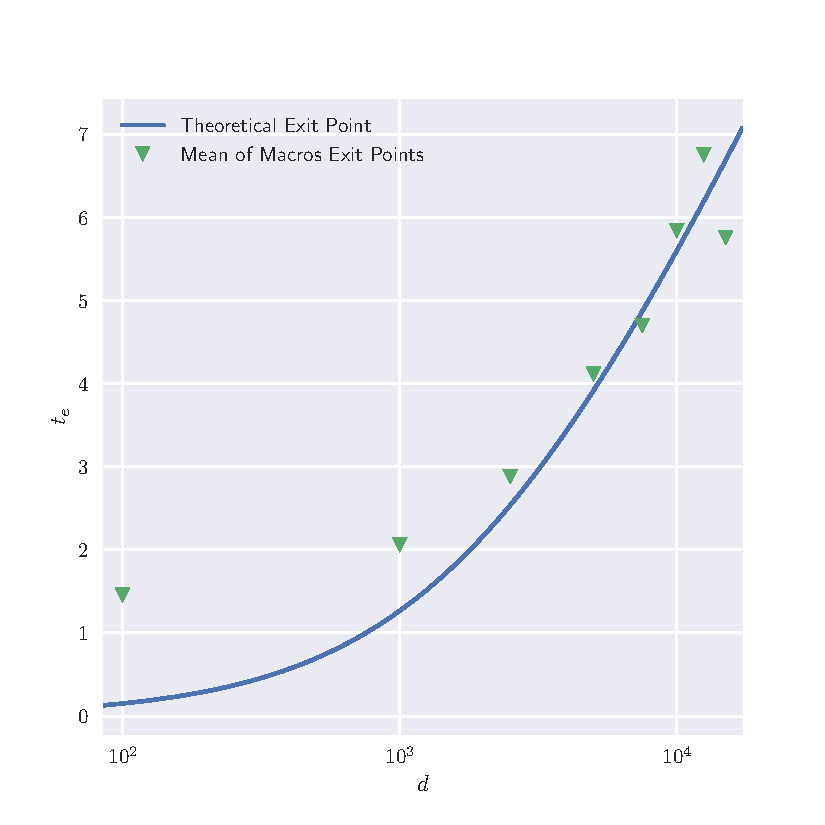
\includegraphics[width=0.9\textwidth]{figures/spherical/phase-retrivial-dplot.pdf}
  \caption{
    simulated exit time for different values of \(d\) compared to \(t^\text{(pr)}_e\).
  }
  \label{fig:spherical-phase-retrivial-with-d}
\end{figure}

\section{Generalized phase retrivial} %\label{sec:first-plateau-on-sphere}
We have just found a formula for exit time in the particular case of phase retrivial and would like to extend it to a generic committee machine.
When \(p\neq1\), in addition to the elements of \(\M\), the non-diagonal entries of \(\Q\) are also variable order parameters;
consequently, the problem becomes more complex to deal with.
We therefore decided to analyze the case \(k=1,p>1\) before moving on to the general case.
The purpose of this model is still to solve the phase retrivial,
but giving the student the opportunity to be able to mediate between different vectors \(\w_j\).

The previous section guides us in the generic case: since all the initial \(\M_j\) and \(\Q_{jl}\) are close to zero,
we can consider only the first order of the Equations~\eqref{eq:genericsphericalM}~and~\eqref{eq:genericsphericalQ}.
The full derivation is in Appendix~\ref{app:derivation-spherical-ode}; the equations are
\begin{subequations}\label{eq:genericsphericalphaseretrivial}\begin{align}
  \dod{\left[\M{\left(t\right)}\right]_{j}}{t} =&
    \left[
      \frac{4 \gamma}{p} -\frac{2 \gamma^2}{p^2} \left(2 +\frac{2}{p} + \frac{8}{p^2} + \Delta \right)
    \right] \left[\M{\left(t\right)}\right]_{j} \\
  %
  \dod{\left[\Q{\left(t\right)}\right]_{jl}}{t} =&
   -\frac{8 \gamma}{p^2} \left[1-\frac{8\gamma}{p^2}\right] \left[\Q{\left(t\right)}\right]_{jl}
\end{align}\end{subequations}
The first observation is that although the equations above represent a system of \(p(p+1)/2\) equations,
they are all independent. What follows is what is a manifestation of \emph{linear learning}: 
in the first stage of learning each hidden unit learns independently of the others.

As a second thing, we observe that again there is a maximum value of the learning rate beyond which there is no learning.
The inequality is found by imposing that \(\M=\vec{0}\) is an unstable equilibrium point of the dynamics
\[
  \frac{4 \gamma}{p} -\frac{2 \gamma^2}{p^2} \left(2 +\frac{2}{p} + \frac{8}{p^2} + \Delta \right) > 0 \quad \implies\quad
  \gamma < \frac{p}{1 +\frac{1}{p} + \frac{4}{p^2} + \frac\Delta2}.
\]
In this case we can get another inequality, by requiring that the non-diagonal \(\Q\) are deacresing in the regime we are analyzing\footnote{
  This request is not necessary, but we still ask it so that the approximate expression of theoretical risk depends on only one exponential.
  It is possible to repeat the analysis even with increasing \(q\)s, but it will not be possible to find a closed formula for exit-time.
  In any case, the inequality on \(\M\) implies that on \(\Q\) except when \(p\in[2,6]\) so the assumption is not unreasonable.
}
\[
  -\frac{8 \gamma}{p^2} \left[1-\frac{8\gamma}{p^2}\right] < 0 \quad \implies\quad
  \gamma < \frac{p^2}{8}.
\]

From Equations~\eqref{eq:genericsphericalphaseretrivial} we can find the approximated evolution of order parameters
\[\begin{split}
  \omega^{(m)}_{\gamma,p} \coloneqq \frac{4 \gamma}{p} -\frac{2 \gamma^2}{p^2} \left(2 +\frac{2}{p} + \frac{8}{p^2} + \Delta \right), \qquad
  m_j{(t)} &= m_j{(0)} \exp\left[\omega^{(m)}_{\gamma,p}t\right] \\
  %
  \omega^{(q)}_{\gamma,p} \coloneqq \frac{8 \gamma}{p^2} \left[1-\frac{8\gamma}{p^2}\right], \qquad
  q_{jl}{(t)} &= q_{jl}{(0)} \exp\left[-\omega^{(q)}_{\gamma,p}t\right]
\end{split}\]

Let's now compute the risk expression in this case. Using Equation~\eqref{eq:risk_quadratic} we get
\[
  \risk{(\Q,\M)} = 1 + \frac1p + \frac{1}{p^2}\sum_{j,l=1;j\neq l}^p q^2_{jl} - \frac2p \sum_{j=1}^p m^2_{j}
\]

As shown in Section~\ref{subsec:initial-condition-phaseretrivial}, all the \(m_j{(0)}\) and the\(q_{jl}{(0)}\) 
are random variables distributed as \(\gauss{(0,d^{-1/2})}\), in the limit of high dimension;
we can therefore compute the expecetd value and the variance of the sum of their squares
\[\begin{split}
 &\E\left[\sum_{j=1}^p m_j^2{(0)}\right] = \frac{p}{d}, \qquad
  \Var\left[\sum_{j=1}^p m_j^2{(0)}\right] = \frac{2p}{d^2}, \\
 &\E\left[\sum_{j,l=1;j\neq l}^p q_{jl}^2{(0)}\right] = \frac{p(p-1)}{d}, \qquad
  \Var\left[\sum_{j=1}^p q_{jl}^2{(0)}\right] = \frac{2p(p-1)}{d^2}. \\
\end{split}\]
We used the fact that all these variables are pairwise independent.
The distribution of these summation is becoming sharper and sharper as you go to the limit \(d\to\infty\),
so we can use the expected values for estimating \(\risk(0)\).
Combing this consideration with the approximated time evolution of the order parameters,
we can write down an approximated evolution for the risk
\[
  \risk_\text{apprx}{(t)} = 1 + \frac1p + \frac{p-1}{pd}\exp{\left[-2\omega^{(q)}_{\gamma,p} t\right]} - \frac2d \exp{\left[2\omega^{(m)}_{\gamma,p} t\right]}
\]
As we did in the previous section, we can derive an exit time by fixing a relative threshold \(T\)
and solve the equation 
\begin{equation}\label{eq:exit_time_equation}
  (1-T)\risk_\text{apprx}{(0)} = \risk_\text{apprx}{\left(t^\text{(gpr)}_e\right)}.
\end{equation}
There is no analytical solution for this equation, but we can compute the root numerically.
In order to arrive at a formula that at least approximates the solution, we will make the additional assumption 
\[
  \exp{\left[-2\omega^{(q)}_{\gamma,p} t^\text{(gpr)}_e\right]}  \approx 0,
\]
which allows us to derive this expression for the exit time
\[
  t^\text{(gpr)}_e = \frac{\log\left[\frac12+\frac{1}{2p}+\frac{T}{2}\left(1+\frac{1}{p}\right)(d-1)\right]}{\frac{8 \gamma}{p} -\frac{4 \gamma^2}{p^2} \left(2 +\frac{2}{p} + \frac{8}{p^2} + \Delta \right)}.
\]
Once again we remark the fact that the formula is scaling logarithmically in \(d\).
Figure~\ref{fig:spherical-generalized-phase-retrivial} shows two example of exit times for different \(p\).

\begin{figure}
  \centering
  \begin{subfigure}{0.8\textwidth}
    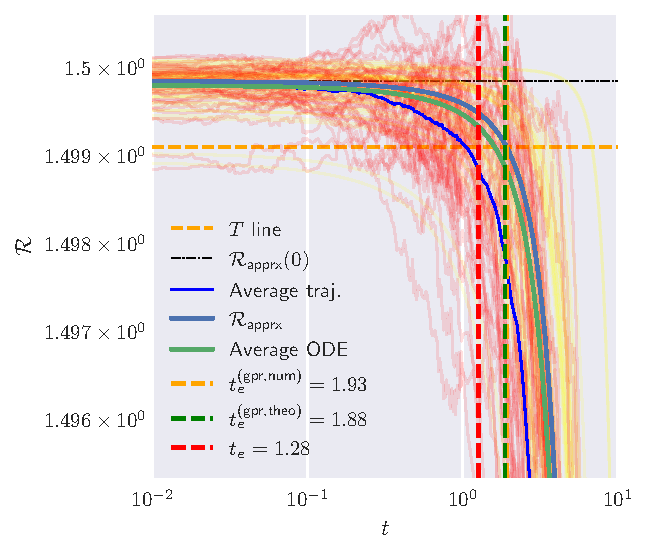
\includegraphics[width=1.\textwidth]{figures/spherical/gpr-p2.pdf}
    \caption{\(p=2\)}
  \end{subfigure}
  \begin{subfigure}{0.8\textwidth}
    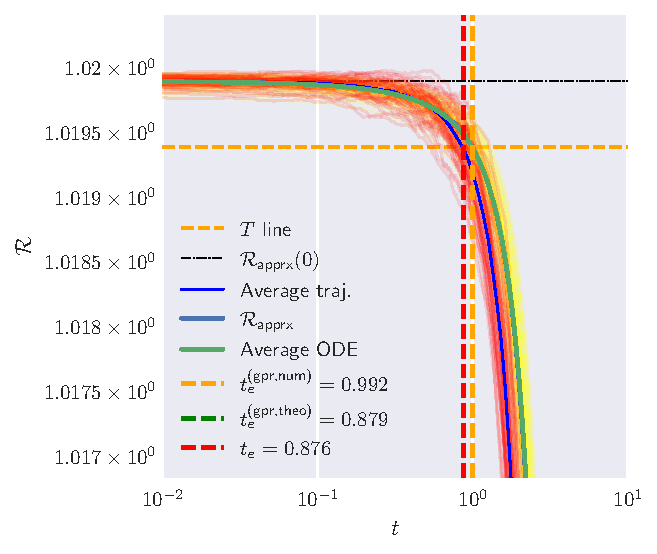
\includegraphics[width=1.\textwidth]{figures/spherical/gpr-p50.pdf}
    \caption{\(p=50\)}
  \end{subfigure}

  \caption{
    example of comparison of two exit times in the generalized phase retrivial; parameters \(\Delta=\num{0.001}, \gamma=0.2p\).
    Both figures are zoomed in on the transition area. It's evident that 
  }
  \label{fig:spherical-generalized-phase-retrivial}
\end{figure}



\subsection{Different regimes}
In this section we will try to push our result further, with the aim of deriving results on the overparametrization of neural networks.
We are aware that the formulas derived are not exact, but contain several approximations,
but we still believe they allow us to make estimates about the benefits of taking a very wide network.

The expression we derived for the exit time is valid for any fixed \(\gamma\) and \(p\).
Our final goal is to dive an empirical prove that there is a gain of performance by overparametrizing the student,
in other words taking \(p\) large. If we keep \(\gamma\) fixed, and we enlarge \(p\), the leading orderd of the exit time 
is \(t_e \propto p\). This is due to the fact that if we have \(p\) weights to learn, thre is a factor \(1/p\) in front of the gradient,
and this makes the process slow down. 

\subsubsection{Fixed $\gamma/p$}
The correct way to compare the learning between student with different \(p\) is to take the learing rate proportional to \(p\)\footnote{
  It's not a problem to enlarge the learning rate, since the update term is of order \(\frac{\gamma}{p}\BigO{1}\), so we will never have too big updates.
}.
Therefore, we define the quantity \[\alpha \coloneqq \frac{\gamma}{p},\] and we keep it costant we comparing exit times.

First of all we can derive some inequalities on the value of \(\alpha\),
which come from the inequalities we derived for the learning rate
\[\begin{split}
  \alpha <& \frac{p}{8} \quad\text{and}\\
  \alpha <& \frac{1}{1 +\frac{1}{p} + \frac{4}{p^2} + \frac\Delta2}.
\end{split}\]
As rule of dumb, if \(\alpha<\frac16\) then both this two are satisfied for every \(p\in[1,+\infty)\)\footnote{
  We remark that if \(p=1\) then the first of the two inequalities is not there since we fall back in the 
  phase retrivial case, where there are no non-diagonal \(\Q\).
}. 

Getting to the point, the expression of exit time rephrased in term of \(\alpha\) is 
\[
  t^\text{(gpr)}_e = \frac{\log\left[\frac12+\frac{1}{2p}+\frac{T}{2}\left(1+\frac{1}{p}\right)(d-1)\right]}{8\alpha} \frac{1}{1- \alpha\left(1+\frac{1}{p}+\frac{4}{p^2}+\frac{\Delta}{2}\right)}
\]
Leaving aside the logarithmic factor, whose dependence on \(p\) is practically irrelevant, 
it's clear that by incresing \(p\) we get a speedup in learning, although it is limited, and does not go to infinity as \(p\) increases.
There is a thoretical limit on the lowest time that can be achivied, even in noiseless situation, with \(p\) as large as possible.
%todo: mettici una figura di come cresce

\subsubsection{Optimal $\alpha$ at every $p$}
We have shown for phase retrivial that there is a theoretical optimal learning rate that makes the exit time minimum.
It's not hard to belive that a similar behaviour is also present in the case \(p>1\),
with a pattern of the \emph{learnig rate--exit time} curve shaped like the one in Figure~\ref{fig:time_learnignrate_plot}.
One objection to what we set forth in the previous section might be that the benefit of overparameterization is only because the increase in \(p\) brings the learning rate closer to the optimal value.
In other words, the decrease in learning time could simply be due to progressively better choice of learning rate as \(p\) changes.
In orderd to debunk this objection, we should compare the time of exists evaluated at the best possible \(\alpha\) for different \(p\).
The calculations for this part are done in this Mathematica notebook.
% todo: metti il link al notebook giusto

As we have done before, we can drop the logarithmic factor from time, keeping only this term
\[
  t{(\alpha,p)} \coloneqq \frac{1}{8\alpha\left[1- \alpha\left(1+\frac{1}{p}+\frac{4}{p^2}+\frac{\Delta}{2}\right)\right]}.
\]
We can now introduce \(\alpha_\text{op}(p)\) as the value of \(\alpha\) that minimizes the time \(t{(\alpha,p)}\) at given \(p\). 
The function \(t{(\alpha,p)}\) is \(\alpha\)-convex in the interval \((0,\alpha_\text{max})\), with \(p\) fixed;
therefore the minimum coorespond to the stationary point
\[
  0 = \eval{\dpd{t{(\alpha,p)}}{\alpha}}_{\alpha = \alpha_\text{op}(p)} \quad\text{leads to}\quad 
  \alpha_\text{op}(p) = \frac{p^2}{(2+\Delta)p^2+2 p+8}.
\]
We can now compute explicitly the best possible learning time at a given \(p\)
\[
  t_\text{opt}{(p)} \coloneqq t{\left(\alpha_\text{op}(p),p\right)} = \frac{(\Delta +2) p^2+2p+8}{4 p^2}.
\]
The most important result is that this is decrasing in \(p\), so the benefits of overparametrization are intact.
Moreover, we can also quantify the gain of overparametrizing the network as the rateo between the phase retrivial case
and the minimum time achievable
\[
  g{(\Delta)} \coloneqq \frac{t_\text{opt}{(1)}}{\lim_{p\to+\infty}t_\text{opt}{(p)}} = \frac{12+\Delta}{2+\Delta} \approx 6.
\]
Although this result is far from exact, we can still infer approximate information about the gain produced by overparameterizing the network.
In particular, we have shown that it is limited and of the order of magnitude of at most tens.
Let us emphasize again how all these results apply only to the first part of the learning;
when the network exits the initial regime, our description no longer applies and it is necessary to change the learning rate to achieve perfect learning.


\section{General Case}
We can extend our analysis to the most general committee machine, where both \(k\) and \(p\) are aribitrary.
The derivation does not include any new idea compared to the generlized phase retrivial

The diferential equations are slightly modified crespect to the prvious ones;
they are derived in Appendix~\ref{app:derivation-spherical-ode} and their final expressions are
\begin{subequations}\label{eq:cm_linearized_odes}\begin{align}
  \dod{\left[\M{\left(t\right)}\right]_{jr}}{t}
    &= \left[
      \frac{4 \gamma}{pk} -\frac{2 \gamma^2}{p^2} \left(\frac2k +\frac{2}{p} + \frac{8}{p^2} + \Delta \right)
    \right] \left[\M{\left(t\right)}\right]_{jr},\\
  \dod{\left[\Q{\left(t\right)}\right]_{jl}}{t} &= -\frac{8 \gamma}{p^2} \left[1-\frac{8\gamma}{p^2}\right] \left[\Q{\left(t\right)}\right]_{jl}.
\end{align}\end{subequations}
One again, the system of equation is fully separated, therefore the only difference between the general case and the previous one is 
the fact that \(\P\) is not a scalar, but a \(k\times k\) matrix instead. The formula for the theoretical risk is
\[
  \risk{(\Q,\M,\P)} = \frac1k + \frac1p + \frac{1}{p^2}\sum_{j,l=1;j\neq l}^p q^2_{jl} - \frac2p \sum_{j=1}^p m^2_{j} + \frac{1}{k^2}\sum_{r,t=1;r\neq t}^k \rho^2_{rt}
\]
Since \(\P\) is the teacher's eigenvector, it is a constant matrix whose entries can be estimated exactly as done with \(\Q(0)\). The initial values of the order parameters become
\[\begin{split}
  &\E\left[\sum_{j=1}^p m_{jr}^2{(0)}\right] = \frac{pk}{d}, \qquad
   \Var\left[\sum_{j=1}^p m_{jr}^2{(0)}\right] = \frac{2pk}{d^2}, \\
  &\E\left[\sum_{r,t=1;r\neq t}^k \rho_{rt}^2{(0)}\right] = \frac{k(k-1)}{d}, \qquad
   \Var\left[\sum_{r,t=1;r\neq t}^k \rho_{rt}^2{(0)}\right] = \frac{2k(k-1)}{d^2}. \\
 \end{split}\]
The approximated risk expression is 
\[
  \risk_\text{apprx}{(t)} = \frac1k + \frac1p + \frac{k-1}{kd} + \frac{p-1}{pd}\exp{\left[-2\omega^{(q)}_{\gamma,p} t\right]} - \frac2d \exp{\left[2\omega^{(m)}_{\gamma,p,k} t\right]}
\]
where \(\omega^{(q)}_{\gamma,p}\) and \(\omega^{(m)}_{\gamma,p,k}\) are properly defined from Equations~\eqref{eq:cm_linearized_odes}.

The exit time can be estimated solving Equation~\eqref{eq:exit_time_equation} with the new approximated risk.
If we want an analytical and approximate expression of the solution,
as before we can neglect the exponential in \(\Q\), yielding
\[t_e = \frac{\log \left[\frac12 + \frac{1}{2p} - \frac{T}{2k} + \frac{dT}{2k} - \frac{T}{2p} + \frac{dT}{2p} \right]}
             {\frac{8 \gamma}{pk} -\frac{4 \gamma^2}{p^2} \left(\frac2k +\frac{2}{p} + \frac{8}{p^2} + \Delta \right)}.
\]

\subsection{Overparameterization gain}
We repeat here the computation of the gain that can be achivied with overparametrization,
using the optimal learning rate at every \(p\).
The full calculations can be found on this Mathematica notebook; 
the bounds on the learning rate are not reported, but they can be found on the notebbok as well.

The optimal value of \(\alpha\) at a given \(p\) is
\[
  \alpha_\text{op}(p) = \frac{p^2}{(2+\Delta k) p^2+2 k p+8 k}
\]
and consequently
\[
  t_\text{opt}{(p)} = \frac{k \left((2+\Delta k) p^2+2 k p+8 k\right)}{4 p^2}.
\]

To conclude, this is the expression for the gain
\[
  g{(\Delta, k)} \coloneqq \frac{t_\text{opt}{(k)}}{\lim_{p\to+\infty}t_\text{opt}{(p)}} =
    \frac{\Delta k^2 + 4k + 8}{\Delta k^2 + 2k},
\]
where of course we used applied the condition \(p\ge k\).
If there is no noise, then the gain is always at least 2; 
if instead the noise it's big then there is no gain at all (even if the learning process would be so slow that the entire training it's useless).
For the last time we emphasize that these results are to be interpreted as estimates of the order of magnitude of the gain achievable by overparameterization.

In the next chapter we will try to refine our results to obtain more precise learning time estimates, but they will obviously lose analytical handling.
  \chapter{Stochasticity of the evolution}
In the previous chapters, we derived an approximated expression for the exit times using the high-dimensional
ordinary differential equations of the process.
The results obtained were only partially satisfactory, as they only partially captured the exit-time trend,
allowing us to make assertions only about the orders of magnitude of the gain obtained by overparameterizing the neural network.

In this chapter we will introduce corrections to the differential equations we have previously used,
transforming them into stochastic differential equations, with the aim of having an exact expression of exit-time.
We will focus only on the phase retrivial, given the simplicity of the equations it involves. 

\section{Stochastic differential equations}
There are two main problems affecting the results on the exit times of previous chapter.
The first one is that the differential equation are valid in the limit~\(d\to+\infty\),
but then we use big, but still finite, \(d\) for comparsion. 
The second problem is that Theorem~\ref{thm:process_to_ode_goldt} explicitly says that the solution of the differential equation approximates the trajectories with an accuracy that scales as \(\frac{1}{\sqrt{d}}\),
which is of the same order as the variation in the order parameters we are trying to measure.
Although we collect some statistics by simulating different trajectories,
the differential equations do not seem to be sufficient to have an accurate estimate of the exit time.

The ordinary differential equations were derived as the limit of a discrete stochastic process.
All random components were cancelled by the limit procedure, leaving simply the expectation value of the random variable.
Rewriting the Equations~\eqref{eq:genericODE}, in the case \(k=p=1\) we have 
\[\begin{split}
  \dod{\left[\M{\left(t\right)}\right]_{11}}{t} &=\E_{\vec{\lf},\vec{\lf^* \sim \gauss{(0,\vec{\Omega}{(t)})}}}{\left[\mathcal{M}\right]} \\
  \dod{\left[\Q{\left(t\right)}\right]_{11}}{t} &=\E_{\vec{\lf},\vec{\lf^* \sim \gauss{(0,\vec{\Omega}{(t)})}}}{\left[\mathcal{Q}\right]},
\end{split}\]
where we have introduced the two random variables
\[\begin{split}
  \mathcal{M} \coloneqq &  \frac{\gamma}{p} \dsp_1 \lf_1^* \\
  \mathcal{Q} \coloneqq &  \frac{\gamma}{p}\left(\dsp_1 \lf_1 + \dsp_1 \lf_1\right) + \frac{\gamma^2}{p^2} \dsp_1^2
\end{split}\]
What we want to do is to include correction terms that incorporate the next order in \(d\).
Obviously, the correction cannot be deterministic since the limit is computed on a random variable;
moreover, it will have to have zero expectation value, otherwise, it would go to change order 0.
The simplest model we can imagine is given by introducing white noise that has as its intensity the standard deviation of the variables on which the expectation values are computed.
In other words, in the passage to the limit, instead of turning the random variables into expectation values,
we instead replace them with Gaussians that best approximate the random variables.
Let's put these considerations into formulas. We can start by defining the covariance matrix of \(\mathcal{M}\)
and \(\mathcal{Q}\)
\[
  \vec{\Sigma} \coloneqq 
  \begin{pmatrix}
    \Var{\left[\mathcal{M}\right]} & \Cov{\left[\mathcal{M},\mathcal{Q}\right]} \\
    \Cov{\left[\mathcal{M},\mathcal{Q}\right]} & \Var{\left[\mathcal{Q}\right]}
  \end{pmatrix},
\]
from which we can define the standard deviation vectors
\[
  \begin{pmatrix}
    \vec{\sigma}_m \\
    \vec{\sigma}_q
  \end{pmatrix}
  \coloneqq
  \sqrt{\vec{\Sigma}}.
\]
We introduce the noise as a differential vector of Wiener processes, one per equation
\[
  \dif \vec{W} \coloneqq 
  \begin{pmatrix}
    \dif W_m \\
    \dif W_q
  \end{pmatrix}
\]
where \(W_m\) and \(W_q\) are 2 indipendent Wiener processes.
What was previously a system of ordinary differential equations now becomes a system of stochastic differential equations.
Referring to Equations~\eqref{eq:genericODE} for notation, and eliminating subscripts since we are focusing on phase retrivial
\begin{subequations}\begin{align}
  \dif m =& \Psi{(m,q)}\dif t + \frac{\vec{\sigma}_m{(m,q)}\cdot\dif \vec{W}}{d} \\
  \dif q =& \Phi{(m,q)}\dif t + \frac{\vec{\sigma}_q{(m,q)}\cdot\dif \vec{W}}{d} 
\end{align}\end{subequations}
Obviously in the limit \(d\to+\infty\) we fall back to ordinary differential equations,
since the stochastic term cancels out.
These equations describe the evolution of the unconstrainted phase retrivial,
which will be the first case we are going to analyze in the next section.

\subsection{Initial conditions}
Before we go to simulate the stochastic process, we must choose what initial conditions to use.
Since our goal is to find a description of the learning process that is able to detect effects that escaped the differential equations,
we will look at the situation where they strayed furthest from the simulation. 
We therefore choose to initialize the phase retrivial with the \emph{symmetric intial conditions with \(\varepsilon = 0\)} (see the \ref{subsec:symmetric_init} section).
In our context we can also assume \(q_0 = 1\): this basically means choosing the vectors \(\w\) and \(\w^*\) as orthogonal.

As already shown, the description with differential equations is not able to break the initial symmetry and the vectors remain orthogonal throughout the process,
changing only the norm of \(\w\).
In contrast, we expect the stochasticity introduced by the corrective term to lead to symmetry breaking and a consequent correct description of the learning process.

Finally we choose to study the case with \(\Delta=0\). 
This choice follows from the fact that in the past chapters we have shown that the value of noise only marginally affects the first part of the process,
i.e., the part we want to study. We therefore choose to exclude it in order to have a less complex,
but no less descriptive, description of the process.
\section{Unconstrainted Phase retrivial}


\section{Spherical Phase retrivial}






  \part{Conclusion}
  \chapter{Summary and future developments}
\subsection*{Summary}
In this work, we have studied two-layers fully-connected neural networks in the teacher-student setting.
We derived deterministic equations for the evolution of the order parameters in the case of the activation function \(\sigma(x)=x^2\),
and pointed out how this may fall into a famous model studied: phase retrieval.
We explored many possible initial conditions and analyzed the symmetries they may introduce.
We arrived at writing an early formula for learning time in the specific case of phase retrieval, noting,
however, that it is not too informative since it is influenced by the norm of the chosen initial conditions.

We then introduced the spherical constraint in order to directly analyze the phases of the learning of our interest.
We derived the differential equations describing the dynamics in this situation and set initial conditions based on what we comprehended previously.
We were able to derive a complete description of phase retrieval dynamics that, among other things,
allowed us to write an explicit formula for an exit time; we verified that it was in agreement with when previously known from the literature.
We then repeated the analysis first for generalized phase retrieval, then for a generic neural network, obtaining discrete results.
We have shown that from learning times it is possible to give an estimate of the gain that is obtained in enlarging the first layer of the network.
By exploring different regimes, we realized that the ratios between the exit time of an overparametized network and one that is not, are finite:
therefore, there is a maximum speed-up that can be achieved, at least at the stage of learning under consideration.

In the last part, we tried to add a corrective term to the equations used for the previous analysis. The added correction is nondeterministic and transforms the equations into stochastic processes, which we approximated through Brownian motions.
For simplicity, we limited ourselves to the phase retrieval analysis. 
First, we applied the corrections to the unconstrained case and showed that they worked and were in agreement with a work that came out in conjunction with our study.
As in the deterministic case, however, we could not derive a formula for exit time. We then moved on to the constrained case on the sphere, where the first difficulty was figuring out how to write the stochastic process.
Through the Itô calculus, we obtained a correct description of the dynamics and,
through the necessary approximations, derived a formula for the exit time.
Comparing the results with those obtained previously from the differential equations,
we found that the corrections allow for a more accurate estimate of the learning time,
leaving several possibilities for future analysis with this tool. 

\subsection*{Future Developments}
There are many directions that can be explored now.
The natural next step to the last part of the results presented in this paper is to derive a description with stochastic processes for the generalized phase retrieval and the generic network as well.
Having more accurate formulas for the output times would allow us to make more precise statements about the gain benefited by overparameterization.
This involves analyzing several stochastic processes, but it should be feasible and has not been analyzed here simply for lack of time.

Another question that arises is whether the analysis done now can be repeated for the specialization phase of learning. Referring to Figure~\ref{fig:pictorial-symmetric-learning2}, we studied the exit time for the blue curve, but not the exit time for the green. 
In the plots of the risk we represented we could see only one drop because with the activation function we chose the two transitions occurred so close together that the plateau between the two is not visible, (besides that this phase is really only present when \(k>1\)). 
One could look for initial conditions that are already in the blue plateau, so as to study only the specialization. Another alternative is to choose a different activation function, where the separation of the two phases is sharper. 
This choice would be beneficial since it would also allow us to use more realistic activation functions such as ReLU or erf.
If the previous goal were to be achieved, one could then consider making the networks deeper and see how the output times relate as a function of the width of the various layers. This is an ambitious task, but a stepwise analysis could lead us to some good results.
\begin{figure}
  \centering
  \begin{tikzpicture}[
    x=1.cm,
    y=1.cm
  ]
    \filldraw [fill=Background,draw opacity=0.] (0,0) rectangle (10.,9.);
\draw[black, ->, thick] (0,0) -- (10,0) node[below] {\(\log t\)};
\draw[black, ->, thick] (0,0) -- (0, 9) node[left] {\(\log\mathcal{R}\)};

\draw[
  line width=1.5mm,
  Red,
  looseness=1.1
] (0,8) to[out=0, in=180]
  (1.0,8) to[out=0, in=180]
  (2., 7) to[out=0, in=180] 
  (10, 7);

\draw[
  line width=1.mm,
  Blue,
  looseness=1.1
] (0,8) to[out=0, in=180]
  (1.0,8) to[out=0, in=180]
  (2., 7) to[out=0, in=180] 
  (4., 7) to[out=0, in=180]
  (5., 5) to[out=0, in=180]
  (10, 5);

\draw[
  line width=0.5mm,
  Green,
  looseness=1.1
] (0,8) to[out=0, in=180]
  (1.0,8) to[out=0, in=180]
  (2., 7) to[out=0, in=180] 
  (4., 7) to[out=0, in=180]
  (5., 5) to[out=0, in=180]
  (6., 5) to[out=0, in=180]
  (8., 1.5) to[out=0, in=180]
  (10., 1.5);

\node[right] at (1.5,7.55) {norm learning};
\node[left] at (4.5,6.) {linear learning};
\node[left] at (7.,3.25) {specialization};
  \end{tikzpicture}
  \caption{
    pictorial representation of the different phases of learning for symmetric initial conditions.
  }
  \label{fig:pictorial-symmetric-learning2}
\end{figure}

Changing perspective, one could study the connections of what we have done with a line of work analyzing the mean-field limit on strongly overparametrized networks \cite{mei2018mean, chizat2018global,rotskoff2018trainability, sirignano2020mean}.
In these papers, they keep fixed the input dimension while they take the limit \(p\to+\infty\);
they find some PDEs on weights probability density that can be used to infer properties of the learning dynamic.
We would therefore like to investigate whether in this different limitation we reach the same conclusions as we do and possibly develop a theory that encapsulates both,
thus arriving at a complete understanding of neural network behavior.

In conclusion, there is still a lot of work to be done within this setting.
This thesis has collected some results that can be expanded and generalized to arrive at a more comprehensive view of two-layer neural networks.
We hope that this work can be a valuable starting point for several future investigations.

  \part*{Appendices}\addcontentsline{toc}{part}{Appendices}
  \appendix
  \pagestyle{appendix-ruled}
  \input{chapters/derivation-quadratic-ODE}
  \chapter[Derivation of linearized spherical ODE]{Derivation of linearized spherical differential equation}
\label{app:derivation-spherical-ode}

\section{Generalized Phase Retrivial}
\begin{equation}
  \Psi_{jr} = \frac{4 \gamma}{p}
      \left(m_{jr} - \frac{m_{jr}}{p}\right) 
      = \frac{4 \gamma}{p} \left(1 - \frac{1}{p}\right) m_{jr},
\end{equation}
while for \(\Phi\) we distinguish the cases \(j=l\) or not
\begin{equation}\begin{split}
  j \neq l \quad \Phi_{jl} &= \frac{4 \gamma}{p}\left[
      2\left( - 2\frac{q_{jl}}{p}\right)
  \right] +\\
  &\quad+\frac{4 \gamma^2}{p^2} \Biggr\{
        3 q_{jl} -\frac2{p}\Biggl[p q_{jl} + 4 q_{jl} \Biggl] + 
        \frac1{p^2}\left[\left(p^2+2p\right)q_{jl} +
        8p q_{jl} + 24q_{jl} \right] + \Delta q_{jl}\Biggr\} \\ 
  &= -\frac{16 \gamma}{p^2} q_{jl} 
    +\frac{4 \gamma^2}{p^2} \left\{
      3 -2 -\frac{8}{p} +1 +\frac2p +\frac8p + \frac{24}{p^2} + \Delta \right\}q_{jl} \\
  &= -\frac{16 \gamma}{p^2} q_{jl} 
  +\frac{4 \gamma^2}{p^2} \left\{2 +\frac{2}{p} + \frac{24}{p^2} + \Delta \right\}q_{jl}
\end{split}\end{equation}
\begin{equation}\begin{split}
  j = l \quad \Phi_{jj} &= \frac{4 \gamma}{p}\left[
      2\left( -\frac{1}{p}\right)
  \right] + \frac{4 \gamma^2}{p^2} \Biggr\{
        3 -\frac2{p}\Biggl[p + 2 \Biggl] + 
        \frac1{p^2}\left[\left(p^2+2p\right) +
        4p + 8 \right] + \Delta\Biggr\} \\
  &= -\frac{8 \gamma}{p^2} + \frac{4 \gamma^2}{p^2} \left\{
    3 -2 -\frac{4}{p} +1 +\frac2p +\frac4p + \frac{8}{p^2} + \Delta \right\} \\
  &= -\frac{8 \gamma}{p^2} +\frac{4 \gamma^2}{p^2} \left\{2 +\frac{2}{p} + \frac{8}{p^2} + \Delta \right\}
\end{split}\end{equation}

Given these linear approximatons, we are ready to write down the equations valid 
as long as the risk stays in the first plateau
\begin{equation}\label{eq:Msphericalgenericpk1}\begin{split}
  \dod{\left[\M{\left(t\right)}\right]_{jr}}{t} &= 
    \left[
      \frac{4 \gamma}{p} \left(1 - \frac{1}{p}\right)
      +\frac{4 \gamma}{p^2}-\frac{2 \gamma^2}{p^2} \left(2 +\frac{2}{p} + \frac{8}{p^2} + \Delta \right)
    \right] \left[\M{\left(t\right)}\right]_{jr} \\
    &= \left[
      \frac{4 \gamma}{p} -\frac{2 \gamma^2}{p^2} \left(2 +\frac{2}{p} + \frac{8}{p^2} + \Delta \right)
    \right] \left[\M{\left(t\right)}\right]_{jr},
\end{split}\end{equation}
\begin{equation}\label{eq:Qsphericalgenericpk1}\begin{split}
  \dod{\left[\Q{\left(t\right)}\right]_{jl}}{t} &= 
    \left[
      -\frac{16 \gamma}{p^2} +\frac{4 \gamma^2}{p^2} \left(2 +\frac{2}{p} + \frac{24}{p^2} + \Delta \right)
      +\frac{8  \gamma}{p^2} -\frac{4 \gamma^2}{p^2}  \left(2 +\frac{2}{p} + \frac{8}{p^2} + \Delta \right)
    \right] \left[\Q{\left(t\right)}\right]_{jl} \\
  &= \left[
    -\frac{8 \gamma}{p^2} +\frac{4 \gamma^2}{p^2} \left(\frac{16}{p^2}\right)
  \right] \left[\Q{\left(t\right)}\right]_{jl} \\
  &= -\frac{8 \gamma}{p^2} \left[1-\frac{8\gamma}{p^2}\right] \left[\Q{\left(t\right)}\right]_{jl}
\end{split}\end{equation}

\section{General case}
The linear expansion of \(\vec{\Phi}\) and \(\vec{\Psi}\) it's similar to previous section:
\[
  \Psi_{jr} = \frac{4 \gamma}{p} \left(\frac1k - \frac{1}{p}\right) m_{jr},
\]\[
  \begin{split}
    j \neq l \quad \Phi_{jl} &= \frac{4 \gamma}{p}\left[
        2\left( - 2\frac{q_{jl}}{p}\right)
    \right] +\\
    &\quad+\frac{4 \gamma^2}{p^2} \Biggr\{
          \left(1+\frac2k\right)q_{jl} -\frac2{pk}\Biggl[pk q_{jl} + 4 k q_{jl} \Biggl] + 
          \frac1{p^2}\left[\left(p^2+2p\right)q_{jl} +
          8p q_{jl} + 24q_{jl} \right] + \Delta q_{jl}\Biggr\} \\ 
    &= -\frac{16 \gamma}{p^2} q_{jl} 
      +\frac{4 \gamma^2}{p^2} \left\{
        1+\frac2k -2 -\frac{8}{p} +1 +\frac2p +\frac8p + \frac{24}{p^2} + \Delta \right\}q_{jl} \\
    &= -\frac{16 \gamma}{p^2} q_{jl} 
    +\frac{4 \gamma^2}{p^2} \left\{\frac2k +\frac{2}{p} + \frac{24}{p^2} + \Delta \right\}q_{jl}
  \end{split}
\]\[
  \begin{split}
    j = l \quad \Phi_{jj} &= \frac{4 \gamma}{p}\left[
        2\left( -\frac{1}{p}\right)
    \right] + \frac{4 \gamma^2}{p^2} \Biggr\{
          \left(1+\frac2k\right) -\frac2{pk}\Biggl[pk + 2k \Biggl] + 
          \frac1{p^2}\left[\left(p^2+2p\right) +
          4p + 8 \right] + \Delta\Biggr\} \\
    &= -\frac{8 \gamma}{p^2} + \frac{4 \gamma^2}{p^2} \left\{
      1+\frac2k -2 -\frac{4}{p} +1 +\frac2p +\frac4p + \frac{8}{p^2} + \Delta \right\} \\
    &= -\frac{8 \gamma}{p^2} +\frac{4 \gamma^2}{p^2} \left\{\frac2k +\frac{2}{p} + \frac{8}{p^2} + \Delta \right\}
  \end{split}
\]
The diferential equations are only a little different
\begin{equation}\begin{split}
  \dod{\left[\M{\left(t\right)}\right]_{jr}}{t}
    &= \left[
      \frac{4 \gamma}{pk} -\frac{2 \gamma^2}{p^2} \left(\frac2k +\frac{2}{p} + \frac{8}{p^2} + \Delta \right)
    \right] \left[\M{\left(t\right)}\right]_{jr},\\
  \dod{\left[\Q{\left(t\right)}\right]_{jl}}{t} &= -\frac{8 \gamma}{p^2} \left[1-\frac{8\gamma}{p^2}\right] \left[\Q{\left(t\right)}\right]_{jl}.
\end{split}\end{equation}
  \chapter[Standard deviation of SDEs]{Standard deviation of stochastic differential equations}
\label{app:std_sde}
In this Appendix we write down the full expression of the varinace and covariance of the variable \(\mathcal{M}\)
and \(\mathcal{Q}\). The goal is to obtain an expression of the matrix \(\vec{\Sigma}\) 
which can then be used to calculate the standard deviations of stochastic processes.

The calculations are long and complicated, for example, they require computing the twelfth moments of a multivariable normal distribution;
we used the generating function technique implemented in this Mathematica Notebook.
%t todo: insert this notebook
\section{Unconstrainted Phase retrivial}
The entries of matrix \(\vec{\Sigma}\) are 
\[\begin{split}
  \Var{[\mathcal{M}]} =& 8 \gamma ^2 \Delta  m^2+4 \gamma ^2 \Delta  q \rho-192 \gamma ^2 m^4+324 \gamma ^2 q^2 m^2+324 \gamma ^2 \rho^2 m^2 \\
                       & -504 \gamma ^2 q \rho m^2+60 \gamma ^2 q \rho^3-72 \gamma ^2 q^2 \rho^2+60 \gamma ^2 q^3 \rho 
\end{split}\]\[\begin{split}
  \Var{[\mathcal{Q}]} =& 128 \gamma ^4 \Delta ^2 q^2+9600 \gamma ^4 \Delta  q^4-2688 \gamma ^4 \Delta  \rho q^3-16512 \gamma ^4 \Delta  m^2 q^2 \\
                       &+768 \gamma ^4 \Delta  \rho^2 q^2+6528 \gamma ^4 \Delta  m^2 \rho q+2304 \gamma ^4 \Delta  m^4+162720 \gamma ^4 q^6-57600 \gamma ^4 \rho q^5 \\
                       &-593280 \gamma ^4 m^2 q^4+28224 \gamma ^4 \rho^2 q^4-13824 \gamma ^4 \rho^3 q^3+473472 \gamma ^4 m^2 \rho q^3+474624 \gamma ^4 m^4 q^2 \\
                       &+4896 \gamma ^4 \rho^4 q^2-254592 \gamma ^4 m^2 \rho^2 q^2+79488 \gamma ^4 m^2 \rho^3 q-336384 \gamma ^4 m^4 \rho q-46080 \gamma ^4 m^6 \\
                       &+78336 \gamma ^4 m^4 \rho^2-1344 \gamma ^3 \Delta  q^3+256 \gamma ^3 \Delta  \rho q^2+1088 \gamma ^3 \Delta  m^2 q-28800 \gamma ^3 q^5 \\
                       &+9024 \gamma ^3 \rho q^4+77376 \gamma ^3 m^2 q^3-3840 \gamma ^3 \rho^2 q^3+1344 \gamma ^3 \rho^3 q^2-49536 \gamma ^3 m^2 \rho q^2 \\
                       &-33024 \gamma ^3 m^4 q+16704 \gamma ^3 m^2 \rho^2 q+10752 \gamma ^3 m^4 \rho+48 \gamma ^2 \Delta  q^2+1536 \gamma ^2 q^4-384 \gamma ^2 \rho q^3 \\
                       &-2688 \gamma ^2 m^2 q^2+128 \gamma ^2 \rho^2 q^2+1088 \gamma ^2 m^2 \rho q+320 \gamma ^2 m^4 
\end{split}\]\[\begin{split}
  \Cov{[\mathcal{M},\mathcal{Q}]} =& 144 \gamma ^3 \Delta  m^3-336 \gamma ^3 \Delta  q^2 m+192 \gamma ^3 \Delta  q \rho m-2880 \gamma ^3 m^5+14544 \gamma ^3 q^2 m^3  \\
                                   &+4752 \gamma ^3 \rho^2 m^3-13536 \gamma ^3 q \rho m^3-7200 \gamma ^3 q^4 m+2448 \gamma ^3 q \rho^3 m \\
                                   &-5184 \gamma ^3 q^2 \rho^2 m+7056 \gamma ^3 q^3 \rho m +24 \gamma ^2 \Delta  q m-912 \gamma ^2 q m^3+432 \gamma ^2 \rho m^3 \\
                                   &+768 \gamma ^2 q^3 m+336 \gamma ^2 q \rho^2 m-624 \gamma ^2 q^2 \rho m.
\end{split}\]

We can also specialize their value to the initial conditions we are using.
In fact, using \(q=1, m=0, \rho=1\) we get
\[\begin{split}
  \Var{[\mathcal{M}]} &= 4 \gamma ^2 \Delta +48 \gamma ^2 \\
  \Var{[\mathcal{Q}]} &= 128 \gamma ^4 \Delta ^2+7680 \gamma ^4 \Delta +124416 \gamma ^4 \\
                      &-1088 \gamma ^3 \Delta -22272 \gamma ^3+48 \gamma ^2 \Delta +1280 \gamma ^2 \\
  \Cov{[\mathcal{M},\mathcal{Q}]} &= 0
\end{split}\]

\section{Spherical Phase retrivial}
\[\begin{split}
  \Var{[\mathcal{M}_S]} =& 144 \gamma ^3 \Delta  m^3-336 \gamma ^3 \Delta  q^2 m+192 \gamma ^3 \Delta  q \rho m-2880 \gamma ^3 m^5+14544 \gamma ^3 q^2 m^3 \\
                         &+4752 \gamma ^3 \rho^2 m^3-13536 \gamma ^3 q \rho m^3-7200 \gamma ^3 q^4 m+2448 \gamma ^3 q \rho^3 m-5184 \gamma ^3 q^2 \rho^2 m \\
                         &+7056 \gamma ^3 q^3 \rho m+24 \gamma ^2 \Delta  q m-912 \gamma ^2 q m^3+432 \gamma ^2 \rho m^3+768 \gamma ^2 q^3 m \\
                         &+336 \gamma ^2 q \rho^2 m-624 \gamma ^2 q^2 \rho m
\end{split}\]
  \chapter{Mathematical tools} \label{app:math_tools}
\section{Stochastic Diffrential Equations}
The aim of this Section is to give a brief introduction on \emph{Stochastic Differential Equations}.
The discussion is not intended to be extremely formal from a mathematical point of view,
but still provide a complete and consistent exposition of the tools used later in the thesis.
For the readers interested in a formal exposition of the concepts expressed below, please refer to \cite{morters2010brownian}.

\subsection{Stochasic Processes}
\begin{Definition}[Stochasic Processes]
  A \emph{stochastich process} is \(\{X_t, t\in T\}\) is a collection of random variable living in the same probability space.
  The set \(T\) is usally considered as the \emph{time domain}, and can be both discrete or continuous.
\end{Definition}

The most fundamental process is the so called \emph{Wiener process}, introduced hereafter.
\begin{Definition}[Wiener Process]
  A continuous stochastich process \(\{W_t\}_{t\ge0}\) is called \emph{Wiener process} if it satisfy these properties:
  \begin{itemize}
    \item \(W_0 = 0\);
    \item The increment is indipendent from past values:
          \[\forall u\ge0: \quad W_{t+u} - W_t  \text{ is indipendent from } W_s \quad \forall s\in[0,t];\]
    \item The increment is distributed as a normal variable with varince equal to time difference:
          \[W_{t+u}-W_t \sim \gauss{(0,u)};\]
    \item The process in continuous in the time:
          \[\] %TODO: find a definition of continuity that suits for us!
  \end{itemize}
\end{Definition}
The importance of this process arise from the fact that it can be used for modelling
most of the stochastich effects that comes from the microscopic action of many agents
external to the modeled system.
In physics context, the Wiener process is often refered as \emph{standard Brownian motion};
moreover, the Wienere process it's used to model the integral white noise.
Lastly, the Wiener process can be derived as continuous limit of a random walk.

\subsection{Integral over a Wiener Process}
Altought a definition of integral for a generic stochastic process is possible,
for this work is interesting only in giving a brief overview of the Wiener process,
because it is the only one needed in the stochasic differential equations of interest.

Let's start from recalling one possible definition of \emph{Riemann Integral} 
of a function \(f\colon[0,T]\to\Real\):
\[
  \int_0^T f{(t)}\dif t \coloneqq \lim_{N\to+\infty} \sum_{k=0}^{N-1}f{(\hat{t}_k)}(t_{k+1}-t_k)
  \quad \text{ with } t_k = \frac{k}{N}T,\,\,\, \hat{t}_k \in [t_k, t_{k+1}].
\]
There exact choices of \(\hat{t}_k\) do not matter, since the limit is converging 
to the same value in any case.

We can now try to extend the Riemann definition to compute the integral of over a Wiener
process. Let \(g:\coloneqq\Real\to\Real\) the function to be integrated. \(g{(t)}\) is a generic (well behaved in some mathematical sense)
random variable depending from time; it's possible to have \(g{(t)} = \tilde{g}{(W_t)}\) or even depending from another stochastic process.
For convinince we will use the convention 
\(\hat{t}_k^\lambda \coloneqq \lambda t_k + (1-\lambda) t_{k+1}\) with \(\lambda\in[0,1]\)\footnote{
  By fixing a value of \(\lambda\) we are essentialy choosing \(\hat{t}_k\) for every 
  interval in the summation. In principle one can think to use different values of \(\lambda\)
  at each different interval, but as it will be clear in a moment, this choice would be
  really impractical and unconvinient.
}. The definition writes as 
\[
  \int_0^T g{(t)}\dif W_t{[\lambda]} \coloneqq \lim_{N\to+\infty} \sum_{k=0}^{N-1}g{(\hat{t}_k^\lambda)}(W_{t_{k+1}}-W_{t_k}).
\]

The first observation to do is that the result won't be a number, as when 
integrating a function, but instead is a random variable, since is calculated as
(limit of) sum of random variables.
\begin{Example}[Integral of Wiener process]
  Let compute the expected value of the integral of \(g{(t)}=2W_t\):
  \[\begin{split}
    \E{\left[\int_0^T 2W_t \dif W_t{[\lambda]}\right]}
      &= \E\left[\lim_{N\to+\infty} \sum_{k=0}^{N-1}2W_{\hat{t}_k^\lambda}(W_{t_{k+1}}-W_{t_k})\right] \\
      &= \E\left[\lim_{N\to+\infty} \sum_{k=0}^{N-1}\left(2W_{\hat{t}_k^\lambda}W_{t_{k+1}}-2W_{\hat{t}_k^\lambda}W_{t_k}
                +(W^2_{t_{k+1}} - W^2_{t_{k+1}}) + (W^2_{\hat{t}_k^\lambda}-W^2_{\hat{t}_k^\lambda}) + (W^2_{t_k}-W^2_{t_k})\right)\right] \\
      &= \E\left[\lim_{N\to+\infty} \sum_{k=0}^{N-1}\left(-(W_{t_{k+1}}-W_{\hat{t}_k^\lambda})^2 + (W_{\hat{t}_k^\lambda}-W_{t_{k}})^2 + (W^2_{t_{k+1}} - W^2_{t_{k}}) \right)\right]
  \end{split}\]
  The first two addend in the summation are always negative (positive), thus we can commute
  the expected value and the summation; the third term is a telescopic sum
  \[\begin{split}
    \E{\left[\int_0^T 2W_t \dif W_t{[\lambda]}\right]}
      &= \lim_{N\to+\infty} \sum_{k=0}^{N-1}\E\left[-(W_{t_{k+1}}-W_{\hat{t}_k^\lambda})^2 + (W_{\hat{t}_k^\lambda}-W_{t_{k}}\right] + \E\left[W^2_{T}\right] \\
      &= \lim_{N\to+\infty} \sum_{k=0}^{N-1}\left(-(t_{k+1}-\hat{t}_k^\lambda) + (\hat{t}_k^\lambda-t_{k})^2\right) + T 
      = T + \lim_{N\to+\infty} \sum_{k=0}^{N-1}\left(-t_{k+1}+2\lambda t_k + 2(1-\lambda)t_{k+1}-t_k\right) \\
      &= T + \lim_{N\to+\infty} \sum_{k=0}^{N-1}(1-2\lambda)(t_{k+1}-t_k) = 2(1-\lambda)T
  \end{split}\]
\end{Example}
It is evident that the choice of \(\lambda\) it's important to define the result.
One can choose infinitly many different stochastich integrations, but the two most common
are \emph{Stratonovich Integration} and \emph{Itô Integration}. They lead to different result,
with different general properties. As presented in the folliwing sections, the choice of a spefic
definition of integration has to be made base on the properties that the modelization requires.

\subsubsection{Stratonovich Integration}
The first definition of integration is the one obtained for \(\lambda=\frac12\).
\begin{Definition}[Stratonovich Integration]
  The \emph{Stratonovich Integration} of a function \(g{(t)}\) over Wiener process is
  \[\int_0^T g{(t)}\circ\dif W_t \coloneqq \lim_{N\to+\infty} \sum_{k=0}^{N-1}g{\left(\frac{t_{k}+t_{k+1}}{2}\right)}(W_{t_{k+1}}-W_{t_k}).\]
\end{Definition}

\subsubsection{Itô Integration}
The second deffirent definition of integration is obtained with \(\lambda=1\).
\begin{Definition}[Itô Integration]
  The second definition of integration is obtained by choosing \(\lambda=1\).
  The \emph{Itô Integration} of a function \(g{(t)}\) over Wiener process is
  \[\int_0^T g{(t)}\dif W_t \coloneqq \lim_{N\to+\infty} \sum_{k=0}^{N-1}g{(t_k)}(W_{t_{k+1}}-W_{t_k}).\]
\end{Definition}

\subsection{Stochastich Differential Equations}
The \emph{stochastic differential equation} arise from the need to describe the
presence of intrisic noise that effects the evolution. Let \(X\) a quantity whose
time evolution is regulated by a determistic term \(\mu{(X,t)}\), as well as a noisy
term \(\xi_t\). We would like to write an equation similar to
\[\dod{X}{t} = \mu{(X,t)} \textcolor{red}{+ \sigma{(X,t)}\xi_t},\]
where the noisy term is highlated because we have not a mathematical definition
of it. Of course \(\xi_t\) must be some sort of stochastic process as defined in 
the previous section. This lead to the first important conclusion: the solution of the
equation will not be a function, but a stochastic process too.

Let try to make the things more formal and give a definition for \(\xi_t\). 
We require the following properties to be satisfied:
\begin{enumerate}
  \item the noise is zero-mean \[\E\left[\xi_t\right] = 0 \quad \forall t;\]
  \item the noise is completelly uncorrelated  \[\E\left[\xi_t\xi_{t'}\right] = 0 \quad \forall t\neq t';\]
  \item the noise is stationary (denoting by \(p\) the probability density function)
        \[p{(\xi_{t_1},\dots,\xi_{t_k})} = p{(\xi_{t_1 + t},\dots,\xi_{t_k + t})} \quad \forall t.\]
\end{enumerate}
The generality is not lost with the first property, since the excpected value produces a drift,
that can be included in the function \(\mu\). Also the third property is not restricting too much 
the type of noise, since \(\sigma\) can incorporate eventual variation of the variance\footnote{
  Of course the property 3 is not just asking to have stationary variance, but the stationarity
  involves the whole distribution.
}. The second property is saying that the noise has no memory of what happened in the past;
the memoryless noise is of course just an approximation of real physics system, but it is still
good enought to model many systems. Moreover, the noise considered in this work is artificially 
generated and it fullsills this property, so the general case is not treated here.







\subsection{Simulation}
\texttt{\href{https://en.wikipedia.org/wiki/Euler–Maruyama_method}}

\subsection{References}
The main source used for the writing of this part are \dots

\section{Generalized Hypergeometric functions}
We include a small appendix where we describe generalized hypergeometric functions.
These functions are often the result of computing statistics on stochastic processes,
such as first passage times.

\begin{Definition}[Pochhammer symbol]
  The Pochhammer symbol of \(a\in\Real\) is defined as 
  \[
    (a)_n \coloneqq \frac{\Gamma(a+n)}{\Gamma(a)},
  \]
  where \(\Gamma\) is the \emph{gamma function} and \(n\ge0\) is an integer.
\end{Definition}

\begin{Definition}[Generalized Hypergeometric function]
  The generalized hypergeometric function \(\prescript{}{p}F_q{\left(a_1,\dots a_p; b_1,\dots,b_q;z\right)}\) is
  \[
    \prescript{}{p}F_q{\left(a_1,\dots a_p; b_1,\dots,b_q;z\right)} =
    \sum_{n=0}^{+\infty} \frac{(a_1)_n\cdots(a_p)_n}{(b_1)_n\cdots(b_q)_n}\frac{z^n}{n!}.
  \]
\end{Definition}


  
  \cleardoublepage
  \nocite{*}
  \pagestyle{acknowledgments}
  \printbibliography[heading=bibintoc]

  \chapter*{Acknowledgments}
  \chaptermark{Acknowledgments}
  \lipsum


\end{document}